\documentclass[onecolumn,10pt,UTF8]{ctexart}

\usepackage[
    hyperfootnotes=true,
    colorlinks=true,
    linkcolor=red,
    anchorcolor=blue,
    citecolor=blue,
    urlcolor=red
]{hyperref}
\usepackage{parallel}% 提供双栏排版支持
\usepackage{graphicx}% 图形支持
\usepackage{geometry}% 用于页面设置
\usepackage{lscape} %页面横置
\usepackage{pdflscape} %页面横置
\usepackage{bm} %公式加粗
\usepackage[fleqn,leqno]{amsmath} %公式
\usepackage{amsfonts}
\usepackage{tabularx}
\usepackage{booktabs}
\usepackage{multirow}
\usepackage{makecell}
\usepackage{threeparttable}
\usepackage{rotating}
\usepackage{longtable}
\usepackage[font=normalsize]{caption}
\usepackage[table]{xcolor}
\usepackage[authoryear,round]{natbib}
%\usepackage{gbt7714}
\usepackage[doipre={doi:~}]{uri}
%\usepackage[none]{hyphenat}%取消英文断词

\renewcommand\tablename{Table}
\renewcommand\figurename{Figure}
\renewcommand\refname{Reference 参考文献}
\newcommand{\tabincell}[2]{\begin{tabular}{@{}#1@{}}#2\end{tabular}} 
\newcommand{\Paragraph}[1]{\vspace{5pt}\noindent\textbf{\large{#1}}\vspace{5pt}}

\geometry{
  a4paper,%
  left = 1.5cm,%
  right = 1.5cm,%
  top = 2.54cm,%
  bottom = 2.54cm%
}%

\tolerance=1000
\emergencystretch=\maxdimen
\hyphenpenalty=5000
\hbadness=10000

\makeatletter
\renewcommand\normalsize{%
\@setfontsize\normalsize\@xpt\@xiipt
\abovedisplayskip 1\p@ \@plus2\p@ \@minus5\p@
\abovedisplayshortskip \z@ \@plus3\p@
\belowdisplayshortskip 6\p@ \@plus3\p@ \@minus3\p@
\belowdisplayskip \abovedisplayskip
\let\@listi\@listI}
\makeatother

\title{\textbf{Transformations and correlations among some clay parameters - the global database\\一些黏土参数之间的转换和相关性 - 全球数据库}}
\date{\today}
\author{Jianye Ching\thanks{
    \textbf{J. Ching}. Department of Civil Engineering, National Taiwan University, Taiwan.
} ~and Kok-Kwang Phoon\thanks{
    \textbf{K.-K. Phoon}. Department of Civil and Environmental Engineering, National University of Singapore, Singapore.
}\thanks{
    \textbf{Corresponding author}: Jianye Ching (e-mail:jyching@gmail.com)
}}

\begin{document}

\maketitle

\section*{Abstract 摘要}

\begin{Parallel}{0.60\textwidth}{}
    \ParallelLText
    {
        This study compiles a large database of 10 clay parameters (labeled as CLAY/10/7490) from 251 studies, covering clay data from 30 regions or countries worldwide. Hence, the range of data covered by this “global” database is broader than that underlying the calibration of existing transformation models in the literature. These transformation models relate test measurements (e.g., cone tip resistance) to appropriate design parameters (e.g., undrained shear strength). The correlation behaviours exhibited by the database among the 10 clay parameters are consistent with those exhibited by existing transformation models in the literature. The biases and transformation uncertainties of these transformation models with respect to the global database are calibrated. It is found that more recent transformation models are less biased and that the transformation uncertainties are typically fairly large. Such large transformation uncertainties are further reduced by incorporating secondary input parameters, such as plasticity index or sensitivity. In a companion paper written by the same authors, a 10-dimensional multivariate probability distribution coupling these clay parameters is constructed from CLAY/10/7490 and a useful application involving updating the entire bivariate probability distribution of two design parameters from three separate measurements is presented.

        \textbf{Key words: }clay properties, correlations, transformation models, database, statistics.
    }
    \ParallelRText
    {
        本研究汇编了来自251个研究的10个粘土参数(标记为CLAY/10/7490)的大型数据库,涵盖了来自全球30个地区或国家的粘土数据。因此,该“全球”数据库所涵盖的数据范围比文献中现有转换模型的标定所依据的范围要广。这些转换模型将测试测量值(例如,锥头阻力)与适当的设计参数(例如,不排水的剪切强度)相关联。数据库显示的10个黏土参数之间的相关行为与文献中现有的转换模型所显示的相关行为一致。这些转换模型相对于全局数据库的偏差和转换不确定性已得到校准。结果发现,更新的转换模型偏差较小,并且转换不确定性通常相当大。通过合并次级输入参数(例如可塑性指数或灵敏度),可以进一步降低如此大的变换不确定性。在同一位作者撰写的伴随论文中,从CLAY/10/7490构建了耦合这些黏土参数的10维多元概率分布,并提出了一个有用的应用程序,其中涉及从三个独立的测量值更新两个设计参数的整个双变量概率分布。

        \textbf{关键词:}黏土特性,相关性,转换模型,数据库,统计数据。
    }
\end{Parallel}

\section{Introduntion 简介}

<<<<<<< HEAD
\begin{paracol}{2}

    Geotechnical variability is a complex attribute that needs careful evaluation. \citet{Phoon1999612} demonstrated using fairly extensive soil statistics that geotechnical variability depends on the site condition, measurement error associated with a field test, and quality of the correlation model adopted to relate the field test to a design property. The first component refers to inherent soil variability, which is customarily categorized as aleatoric in nature because it cannot be reduced by performing more tests. The second and third components, namely measurement error inevitably introduced in a test procedure and data scatter about a mean correlation trend (typically in the form of a linear regression equation), are customarily categorized epistemic in nature. They can be reduced by gathering more data or building better models. While there are merits to categorizing uncertainties as aleatoric or epistemic, one should be mindful that this demarcation is in part a modeler’s choice \citep{DerKiureghian2007}. From a practical perspective, it is perhaps more important to align tatistical characterization to the property evaluation procedure already embedded in our geotechnical engineering practice. In recognition of the need to respect sound geotechnical engineering practice, \citet{Phoon1999625} presented guidelines for coefficients of variation (COVs) of some soil properties as a function of the test method, correlation equation, and soil type. The key conclusion in this study is that it is not possible to assign a single coefficient of variation (COV) to a design property, such as the undrained shear strength. Geotechnical reliability-based design (RBD) equations that are calibrated using this single COV assumption are too simplistic, because diverse methodologies in estimating soil properties are ignored. This diversity is actually good practice, because there is a need to accommodate diverse site conditions. \citet{Phoon1999612,Phoon1999625} advocated that the calibration of geotechnical RBD equations should be carried out in explicit recognition of property variability and in full compliance with how soil properties are physically evaluated in practice. The framework recommended by \citet{Phoon1999612,Phoon1999625} and the ensuing three-tier classification scheme of soil property variability \citep{Phoon2008344} should be viewed as the minimum requirements in variability characterization. The third edition of ISO 2394 (General principles on reliability for structures; to be published in 2015) includes a new Annex D on “Reliability of geotechnical structures” where the importance of respecting sound geotechnical engineering practices in variability characterization and reliability calibration is strongly emphasized.

    \switchcolumn

    岩土变异性是一个复杂的属性,需要仔细评估。 \citet{Phoon1999612}使用相当广泛的土体统计数据证明,岩土工程变异性取决于现场条件,与现场测试相关的测量误差以及将现场测试与设计属性相关联的相关模型的质量。第一部分是土体固有的变异性,由于无法通过执行更多的测试来减少,因此习惯上被归类为无酸。第二和第三部分,即不可避免地在测试过程中引入的测量误差和关于平均相关趋势的数据散布(通常以线性回归方程的形式),本质上通常被归类为认识论。可以通过收集更多数据或建立更好的模型来减少它们。尽管将不确定性归类为偶然性或认知性是有好处的,但应该记住,这种划分在某种程度上是建模者的选择\citep{DerKiureghian2007}。从实践的角度来看,将地物特征与已经嵌入到我们的岩土工程实践中的属性评估程序对齐可能更为重要。考虑到需要尊重合理的岩土工程实践,\citet{Phoon1999625}提出了一些土体特性的变异系数(COV)的准则,这些准则是测试方法,相关方程和土体类型的函数。这项研究的关键结论是,不可能为设计特性(例如不排水的剪切强度)分配单个变异系数(COV)。使用这种单一COV假设进行校准的基于岩土工程的基于可靠性的设计(RBD)方程过于简单,因为忽略了估算土体性质的多种方法。实际上,这种多样性是一种好习惯,因为有必要适应各种现场条件。 \citet{Phoon1999612,Phoon1999625}提倡,对岩土工程RBD方程的标定应在明确认识到物性变异性的前提下进行,并完全符合实际中对土体物性的评估方法。 \citet{Phoon1999612,Phoon1999625}建议的框架和随后的三层土体性质变异性分类方案\citep{Phoon2008344}应被视为变异性表征的最低要求。 ISO 2394第三版(关于结构可靠性的一般原则;将于2015年发布)包括有关“岩土结构可靠性”的新附件D,在该附录D中,强烈强调了在变异性表征和可靠性校准中尊重岩土工程实践的重要性。

    \switchcolumn*

    The characterization of geotechnical variability is far from being a mature area in research. An astute practitioner would readily point out that multiple tests are commonly conducted in a site investigation and it is common practice to estimate a design property from these tests, either by straightforward averaging or picking a credible worst-case value from the range of values produced by different tests. The information collected in a site investigation programme is fundamentally multivariate in nature and this aspect has not been considered in the earlier studies mentioned above. The purpose of this paper is to develop unbiased transformation models and to quantify their associated uncertainties for 10 common clay parameters. A companion paper \citep{Ching2014686} develops a multivariate probability model coupling these clay parameters. The supporting database contains information from multiple tests that are collected in close proximity. Inother words, each data point records soil information at a specific location and depth, i.e., at a specific sampling point. Note that measurement error is present, but it is not possible to isolate measurement error from transformation uncertainty in conventional site investigation programs. Hence, the transformation uncertainties presented in this study include some measurement errors, but these errors are relatively minor for cone penetration testing with pore pressure measurement (CPTU) \citep{Phoon1999612}. Inherent soil variability is clearly not considered in this study. In principle, inherent soil variability can be incorporated by extending the multivariate probability model (whichapplies to a sampling “point”) to a vector random field covering the three-dimensional (3D) spatial domain of the entire site. The outcomes of this study are thus incomplete in this sense, but they can be viewed as paving the way for characterization of geotechnical variability to advance beyond univariate data and to achieve closer alignment to how soil properties are estimated in actual practice from site investigation programs.

    \switchcolumn

    岩土工程变异性的表征还远远不是研究的成熟领域。精明的从业人员会很容易地指出,在现场调查中通常会进行多次测试,并且通常的做法是根据这些测试来评估设计属性,方法是直接取平均值,或者从测试产生的值的范围内选择可信的最坏情况下的值。不同的测试。在现场调查程序中收集的信息本质上本质上是多元的,并且在上述早期研究中并未考虑到这方面。本文的目的是为10个常见黏土参数建立无偏转换模型并量化其相关的不确定性。伴随论文\citep{Ching2014686}开发了耦合这些粘土参数的多元概率模型。支持数据库包含来自紧密收集的多个测试的信息。换句话说,每个数据点记录特定位置和深度,即特定采样点的土体信息。请注意,存在测量误差,但是在传统的站点调查程序中无法将测量误差与变换不确定性区分开。因此,本研究中提出的变换不确定性包括一些测量误差,但是对于使用孔隙压力测量(CPTU)进行的圆锥渗透测试,这些误差相对较小\citep{Phoon1999612}。这项研究显然没有考虑土体固有的变异性。原则上,可以通过将多元概率模型(适用于采样“点”)扩展到覆盖整个站点的三维(3D)空间域的向量随机字段来合并固有的土体可变性。因此,从这个意义上说,这项研究的结果是不完整的,但可以认为它们为表征岩土工程变异性铺平了道路,使岩土变异性超越了单变量数据,并与现场调查程序在实际实践中对土体特性的估算更加接近。

    \switchcolumn*

    As noted by \citet{Phoon1999612}, the measurement from a geotechnical test is typically not directly applicable to design. Instead, a transformation model is needed to relate the test measurement to an appropriate design parameter. Most transformation models in geotechnical engineering are obtained by empirical or semi-empirical data-fitting using regression analyses. These transformation models are widely adopted in geotechnical engineering practice as a matter of practical expediency. Useful compilations of these models (mostly pairwise correlations) are available in the literature (e.g., \citealp{Kulhawy1990}; \citealp{Mayne2001}). A cursory review of these compilations would reveal a rather bewildering variety and number of models. Most models were developed for a specific geomaterial type and (or) a specific locale.

    \switchcolumn

    正如\citet{Phoon1999612}指出的那样,岩土试验的测量结果通常不适用于设计。 取而代之的是,需要一个转换模型来将测试度量与适当的设计参数相关联。 岩土工程中的大多数转换模型都是通过使用回归分析的经验或半经验数据拟合获得的。 出于实际考虑,这些转换模型已在岩土工程实践中广泛采用。 这些模型的有用汇编(主要是成对相关)可在文献中找到(例如\citealp{Kulhawy1990}; \citealp{Mayne2001})。 粗略地回顾一下这些汇编,将会发现令人困惑的各种模型。 大多数模型是针对特定的土工材料类型和(或)特定的区域设置而开发的。

    \switchcolumn*

    It is not judicious to apply these models indiscriminately to other sites without a proper appreciation of geomaterial behaviour and geology. This “site-specific” limitation is a distinctive and fundamental feature of geotechnical engineering practice. Geotechnical design must take cognizance of this limitation to avoid gross oversimplification of “ground truths.” As opposed to site-specific models, \citet{Ching201252} demonstrated the construction of “global” models. Global models are calibrated from global databases covering many sites and geomaterial types. \citet{Ching201252} observed that site-specific models are generally more precise than global models, but they can be significantly biased when applied to another site. On the contrary, global models are less precise than site-specific models, but they are less biased. Their observations are already well appreciated by engineers. The key contribution from \citet{Ching201252} was to demonstrate these observations with statistical rigor using a sizeable global database.

    \switchcolumn

    在没有适当了解地球物质行为和地质的情况下,不加选择地将这些模型应用于其他地点并不明智。这种“特定于地点”的限制是岩土工程实践的独特和基本特征。岩土设计必须意识到这一局限性,以避免对“地面真相”的过分简化。与特定地点的模型相反,\citet{Ching201252}演示了“全局”模型的构建。全局模型是根据覆盖许多站点和岩土材料类型的全局数据库进行校准的。 \citet{Ching201252}观察到,特定于站点的模型通常比全局模型更为精确,但将其应用于其他站点时可能会出现明显偏差。相反,全局模型不如特定于站点的模型精确,但它们的偏向性较小。他们的观察已经得到工程师的赞赏。\citet{Ching201252}的主要贡献是使用庞大的全球数据库以严格的统计数据证明了这些观察结果。

    \switchcolumn*

    Because most transformation models were built based on their own databases, their ranges of application are, in principle, limited to the range of characteristics contained in the databases, e.g., certain soil types, certain range of soil properties (e.g., insensitive clays), and certain geographic locations. It is important to assess their biases and the uncertainties when these models are applied globally (i.e., applying these models outside their range of calibration). In the current paper, a global clay database is compiled and presented. This database consists of data points from 251 studies, covering clay data from 30 regions or countries worldwide. Hence, the range of data covered by this “global” database is broader than that underlying the calibration of existing transformation models in the literature. Ten parameters of clays are of main interest, including three index properties (i.e., Atterberg’s limits); four parameters for effective stresses, shear strength, and sensitivity; and three parameters from piezocone tests (CPTU). This global database is the largest database compiled by the authors thus far in terms of number of data points and number of parameters of interest. \autoref{table:1} shows the databases compiled by the authors, labeled as (soil type)/(number of parameters of interest)/(number of data points). The current global database is CLAY/10/7490. The first purpose of this paper is to present this large database and verify whether the correlation behaviours in the data points are consistent with those exhibited by existing transformation models in the literature. Most of these models are sitespecific models. The biases and uncertainties in these models will be estimated using the global database. The site-specific models can be applied to a wider range of conditions when their biases are corrected and their transformation uncertainties are  uitably revised.

    \switchcolumn

    由于大多数转化模型都是基于其自身的数据库构建的,因此,其应用范围原则上仅限于数据库中包含的特征范围,例如某些土体类型,某些土体特性范围(例如不敏感的粘土),和某些地理位置。在全球范围内应用这些模型时(即在校准范围之外应用这些模型),评估它们的偏差和不确定性很重要。在当前的论文中,一个全球粘土数据库被编译并呈现出来。该数据库包含来自251个研究的数据点,涵盖了来自全球30个地区或国家的粘土数据。因此,该“全球”数据库所涵盖的数据范围比文献中现有转换模型的标定所依据的范围要广。黏土的10个主要参数是我们关注的重点,其中包括三个指数属性(即,阿特伯格极限);有效应力,剪切强度和灵敏度的四个参数;以及压电锥测试(CPTU)的三个参数。就数据点的数量和感兴趣的参数的数量而言,该全局数据库是迄今为止作者编写的最大的数据库。\cntableref{table:1}显示了作者编译的数据库,标记为(土体类型)/(感兴趣的参数数量)/(数据点数量)。当前的全局数据库是CLAY/10/7490。本文的首要目的是介绍这个大型数据库,并验证数据点中的相关行为是否与文献中现有转换模型所显示的行为一致。这些模型大多数是特定于站点的模型。这些模型中的偏差和不确定性将使用全球数据库进行估算。当特定位置的模型的偏差得到纠正并且适当地修改了转换不确定性时,可以将其应用于更广泛的条件。

=======
\begin{Parallel}{0.60\textwidth}{}
    \ParallelLText
    {
        Geotechnical variability is a complex attribute that needs careful evaluation. \citet{Phoon1999612} demonstrated using fairly extensive soil statistics that geotechnical variability depends on the site condition, measurement error associated with a field test, and quality of the correlation model adopted to relate the field test to a design property. The first component refers to inherent soil variability, which is customarily categorized as aleatoric in nature because it cannot be reduced by performing more tests. The second and third components, namely measurement error inevitably introduced in a test procedure and data scatter about a mean correlation trend (typically in the form of a linear regression equation), are customarily categorized epistemic in nature. They can be reduced by gathering more data or building better models. While there are merits to categorizing uncertainties as aleatoric or epistemic, one should be mindful that this demarcation is in part a modeler’s choice \citep{DerKiureghian2007}. From a practical perspective, it is perhaps more important to align tatistical characterization to the property evaluation procedure already embedded in our geotechnical engineering practice. In recognition of the need to respect sound geotechnical engineering practice, \citet{Phoon1999625} presented guidelines for coefficients of variation (COVs) of some soil properties as a function of the test method, correlation equation, and soil type. The key conclusion in this study is that it is not possible to assign a single coefficient of variation (COV) to a design property, such as the undrained shear strength. Geotechnical reliability-based design (RBD) equations that are calibrated using this single COV assumption are too simplistic, because diverse methodologies in estimating soil properties are ignored. This diversity is actually good practice, because there is a need to accommodate diverse site conditions. \citet{Phoon1999612,Phoon1999625} advocated that the calibration of geotechnical RBD equations should be carried out in explicit recognition of property variability and in full compliance with how soil properties are physically evaluated in practice. The framework recommended by \citet{Phoon1999612,Phoon1999625} and the ensuing three-tier classification scheme of soil property variability \citep{Phoon2008344} should be viewed as the minimum requirements in variability characterization. The third edition of ISO 2394 (General principles on reliability for structures; to be published in 2015) includes a new Annex D on “Reliability of geotechnical structures” where the importance of respecting sound geotechnical engineering practices in variability characterization and reliability calibration is strongly emphasized.
    }
    \ParallelRText
    {
        岩土变异性是一个复杂的属性,需要仔细评估。 \citet{Phoon1999612}使用相当广泛的土体统计数据证明,岩土工程变异性取决于现场条件,与现场测试相关的测量误差以及将现场测试与设计属性相关联的相关模型的质量。第一部分是土体固有的变异性,由于无法通过执行更多的测试来减少,因此习惯上被归类为无酸。第二和第三部分,即不可避免地在测试过程中引入的测量误差和关于平均相关趋势的数据散布(通常以线性回归方程的形式),本质上通常被归类为认识论。可以通过收集更多数据或建立更好的模型来减少它们。尽管将不确定性归类为偶然性或认知性是有好处的,但应该记住,这种划分在某种程度上是建模者的选择\citep{DerKiureghian2007}。从实践的角度来看,将地物特征与已经嵌入到我们的岩土工程实践中的属性评估程序对齐可能更为重要。考虑到需要尊重合理的岩土工程实践,\citet{Phoon1999625}提出了一些土体特性的变异系数(COV)的准则,这些准则是测试方法,相关方程和土体类型的函数。这项研究的关键结论是,不可能为设计特性(例如不排水的剪切强度)分配单个变异系数(COV)。使用这种单一COV假设进行校准的基于岩土工程的基于可靠性的设计(RBD)方程过于简单,因为忽略了估算土体性质的多种方法。实际上,这种多样性是一种好习惯,因为有必要适应各种现场条件。 \citet{Phoon1999612,Phoon1999625}提倡,对岩土工程RBD方程的标定应在明确认识到物性变异性的前提下进行,并完全符合实际中对土体物性的评估方法。 \citet{Phoon1999612,Phoon1999625}建议的框架和随后的三层土体性质变异性分类方案\citep{Phoon2008344}应被视为变异性表征的最低要求。 ISO 2394第三版(关于结构可靠性的一般原则;将于2015年发布)包括有关“岩土结构可靠性”的新附件D,在该附录D中,强烈强调了在变异性表征和可靠性校准中尊重岩土工程实践的重要性。
    }
    \ParallelPar
    \ParallelLText
    {
        The characterization of geotechnical variability is far from being a mature area in research. An astute practitioner would readily point out that multiple tests are commonly conducted in a site investigation and it is common practice to estimate a design property from these tests, either by straightforward averaging or picking a credible worst-case value from the range of values produced by different tests. The information collected in a site investigation programme is fundamentally multivariate in nature and this aspect has not been considered in the earlier studies mentioned above. The purpose of this paper is to develop unbiased transformation models and to quantify their associated uncertainties for 10 common clay parameters. A companion paper \citep{Ching2014686} develops a multivariate probability model coupling these clay parameters. The supporting database contains information from multiple tests that are collected in close proximity. Inother words, each data point records soil information at a specific location and depth, i.e., at a specific sampling point. Note that measurement error is present, but it is not possible to isolate measurement error from transformation uncertainty in conventional site investigation programs. Hence, the transformation uncertainties presented in this study include some measurement errors, but these errors are relatively minor for cone penetration testing with pore pressure measurement (CPTU) \citep{Phoon1999612}. Inherent soil variability is clearly not considered in this study. In principle, inherent soil variability can be incorporated by extending the multivariate probability model (whichapplies to a sampling “point”) to a vector random field covering the three-dimensional (3D) spatial domain of the entire site. The outcomes of this study are thus incomplete in this sense, but they can be viewed as paving the way for characterization of geotechnical variability to advance beyond univariate data and to achieve closer alignment to how soil properties are estimated in actual practice from site investigation programs
    }
    \ParallelRText
    {
        岩土工程变异性的表征还远远不是研究的成熟领域。精明的从业人员会很容易地指出,在现场调查中通常会进行多次测试,并且通常的做法是根据这些测试来评估设计属性,方法是直接取平均值,或者从测试产生的值的范围内选择可信的最坏情况下的值。不同的测试。在现场调查程序中收集的信息本质上本质上是多元的,并且在上述早期研究中并未考虑到这方面。本文的目的是为10个常见黏土参数建立无偏转换模型并量化其相关的不确定性。伴随论文\citep{Ching2014686}开发了耦合这些粘土参数的多元概率模型。支持数据库包含来自紧密收集的多个测试的信息。换句话说,每个数据点记录特定位置和深度,即特定采样点的土体信息。请注意,存在测量误差,但是在传统的站点调查程序中无法将测量误差与变换不确定性区分开。因此,本研究中提出的变换不确定性包括一些测量误差,但是对于使用孔隙压力测量(CPTU)进行的圆锥渗透测试,这些误差相对较小\citep{Phoon1999612}。这项研究显然没有考虑土体固有的变异性。原则上,可以通过将多元概率模型(适用于采样“点”)扩展到覆盖整个站点的三维(3D)空间域的向量随机字段来合并固有的土体可变性。因此,从这个意义上说,这项研究的结果是不完整的,但可以认为它们为表征岩土工程变异性铺平了道路,使岩土变异性超越了单变量数据,并与现场调查程序在实际实践中对土体特性的估算更加接近。
    }
    \ParallelPar
    \ParallelLText
    {
        As noted by \citet{Phoon1999612}, the measurement from a geotechnical test is typically not directly applicable to design. Instead, a transformation model is needed to relate the test measurement to an appropriate design parameter. Most transformation models in geotechnical engineering are obtained by empirical or semi-empirical data-fitting using regression analyses. These transformation models are widely adopted in geotechnical engineering practice as a matter of practical expediency. Useful compilations of these models (mostly pairwise correlations) are available in the literature (e.g., \citealp{Kulhawy1990}; \citealp{Mayne2001}). A cursory review of these compilations would reveal a rather bewildering variety and number of models. Most models were developed for a specific geomaterial type and (or) a specific locale.
    }
    \ParallelRText
    {
        正如\citet{Phoon1999612}指出的那样,岩土试验的测量结果通常不适用于设计。 取而代之的是,需要一个转换模型来将测试度量与适当的设计参数相关联。 岩土工程中的大多数转换模型都是通过使用回归分析的经验或半经验数据拟合获得的。 出于实际考虑,这些转换模型已在岩土工程实践中广泛采用。 这些模型的有用汇编(主要是成对相关)可在文献中找到(例如\citealp{Kulhawy1990}; \citealp{Mayne2001})。 粗略地回顾一下这些汇编,将会发现令人困惑的各种模型。 大多数模型是针对特定的土工材料类型和(或)特定的区域设置而开发的。
    }
    \ParallelPar
    \ParallelLText
    {
        It is not judicious to apply these models indiscriminately to other sites without a proper appreciation of geomaterial behaviour and geology. This “site-specific” limitation is a distinctive and fundamental feature of geotechnical engineering practice. Geotechnical design must take cognizance of this limitation to avoid gross oversimplification of “ground truths.” As opposed to site-specific models, \citet{Ching201252} demonstrated the construction of “global” models. Global models are calibrated from global databases covering many sites and geomaterial types. \citet{Ching201252} observed that site-specific models are generally more precise than global models, but they can be significantly biased when applied to another site. On the contrary, global models are less precise than site-specific models, but they are less biased. Their observations are already well appreciated by engineers. The key contribution from \citet{Ching201252} was to demonstrate these observations with statistical rigor using
        a sizeable global database.
    }
    \ParallelRText
    {
        在没有适当了解地球物质行为和地质的情况下,不加选择地将这些模型应用于其他地点并不明智。这种“特定于地点”的限制是岩土工程实践的独特和基本特征。岩土设计必须意识到这一局限性,以避免对“地面真相”的过分简化。与特定地点的模型相反,\citet{Ching201252}演示了“全局”模型的构建。全局模型是根据覆盖许多站点和岩土材料类型的全局数据库进行校准的。 \citet{Ching201252}观察到,特定于站点的模型通常比全局模型更为精确,但将其应用于其他站点时可能会出现明显偏差。相反,全局模型不如特定于站点的模型精确,但它们的偏向性较小。他们的观察已经得到工程师的赞赏。\citet{Ching201252}的主要贡献是通过使用
    }
    \ParallelPar
    \ParallelLText
    {
        Because most transformation models were built based on their own databases, their ranges of application are, in principle, limited to the range of characteristics contained in the databases, e.g., certain soil types, certain range of soil properties (e.g., insensitive clays), and certain geographic locations. It is important to assess their biases and the uncertainties when these models are applied globally (i.e., applying these models outside their range of calibration). In the current paper, a global clay database is compiled and presented. This database consists of data points from 251 studies, covering clay data from 30 regions or countries worldwide. Hence, the range of data covered by this “global” database is broader than that underlying the calibration of existing transformation models in the literature. Ten parameters of clays are of main interest, including three index properties (i.e., Atterberg’s limits); four parameters for effective stresses, shear strength, and sensitivity; and three parameters from piezocone tests (CPTU). This global database is the largest database compiled by the authors thus far in terms of number of data points and number of parameters of interest. Table \ref{table:1} shows the databases compiled by the authors, labeled as (soil type)/(number of parameters of interest)/(number of data points). The current global database is CLAY/10/7490. The first purpose of this paper is to present this large database and verify whether the correlation behaviours in the data points are consistent with those exhibited by existing transformation models in the literature. Most of these models are sitespecific models. The biases and uncertainties in these models will be estimated using the global database. The site-specific models can be applied to a wider range of conditions when their biases are corrected and their transformation uncertainties are  uitably revised.
    }
    \ParallelRText
    {
        由于大多数转化模型都是基于其自身的数据库构建的,因此,其应用范围原则上仅限于数据库中包含的特征范围,例如某些土体类型,某些土体特性范围(例如不敏感的粘土),和某些地理位置。在全球范围内应用这些模型时(即在校准范围之外应用这些模型),评估它们的偏差和不确定性很重要。在当前的论文中,一个全球粘土数据库被编译并呈现出来。该数据库包含来自251个研究的数据点,涵盖了来自全球30个地区或国家的粘土数据。因此,该“全球”数据库所涵盖的数据范围比文献中现有转换模型的标定所依据的范围要广。十个主要参数是黏土,其中包括三个指数属性(即,阿特伯格极限);有效应力,剪切强度和灵敏度的四个参数;以及压电锥测试(CPTU)的三个参数。就数据点的数量和感兴趣的参数的数量而言,该全局数据库是迄今为止作者编写的最大的数据库。表\ref{table:1}显示了作者编译的数据库,标记为(土体类型)/(感兴趣的参数数量)/(数据点数量)。当前的全局数据库是CLAY/10/7490。本文的首要目的是介绍这个大型数据库,并验证数据点中的相关行为是否与文献中现有转换模型所显示的行为一致。这些模型大多数是特定于站点的模型。这些模型中的偏差和不确定性将使用全球数据库进行估算。当特定位置的模型的偏差得到纠正并且适当地修改了转换不确定性时,可以将其应用于更广泛的条件。
    }
    \ParallelPar
>>>>>>> parent of 34d827c... Ching2014
    \begin{table*}[!htb]
    \centering
    \footnotesize
    \caption{Databases compiled by the authors.}
    \addtocounter{table}{-1}
    \vspace{-8pt}
    \renewcommand{\tablename}{表}
    \caption{作者编译的数据库。}
    \vspace{4pt}
    \renewcommand{\tablename}{Table}
    \setlength{\tabcolsep}{1mm}{
    \begin{tabularx}{\textwidth}{XlllllXX}
        \toprule
        \multirow{2}{*}{Database}  & \multirow{2}{*}{Reference}  &  \multirow{2}{*}{Parameters of interest}  &  \multirow{2}{*}{\shortstack{No. of \\data \\points}}    &  \multirow{2}{*}{\shortstack{No. of \\sites or \\studies}}    & \multicolumn{3}{l}{Range of Properties} \\
             &         &     	 &     &     & OCR   & PI      & $S_t$ \\
        \midrule
        CLAY/5/345      & \citet{Ching2012522}  & $\rm{LI},s_u,s_u^{re},\sigma_p',\sigma_v'$        									    & 345   		    &   37 sites    		 & 1$\sim$4   & -     			& \tabincell{l}{Sensitive to \\quick clays} \\
        \specialrule{0em}{2pt}{2pt}
        CLAY/6/535      & \citet{Ching201477}   & \tabincell{l}{$s_u/\sigma_v',\rm{OCR},(q_t-s_v)/\sigma_v',$\\$(q_t-u_2)/\sigma_v',(u_2-u_0)/\sigma_v',B_q$}      				    & 535   		    &   40 sites    		 & 1$\sim$6   & \tabincell{l}{Low to very \\high plasticity}  & \tabincell{l}{Insensitive to \\quick clays} \\
        \specialrule{0em}{2pt}{2pt}
        CLAY/7/6310     & \citet{Ching2013907}  & \tabincell{l}{$s_u~\rm{under~seven~different~}s_u~$\\$\rm{test~types}$}      								    & 6310  		    &   164 studies   		 & 1$\sim$10  & \tabincell{l}{Low to very \\high plasticity}  & \tabincell{l}{Insensitive to \\quick clays} \\
        \specialrule{0em}{2pt}{2pt}
        CLAY/10/7490    & This paper            & \tabincell{l}{$\rm{LL},\rm{PI},\rm{LI},\sigma_v'/P_a,\sigma_p'/P_a,$\\$s_u/\sigma_v',S_t,(q_t-\sigma_v)/\sigma_v',$\\$(q_t-u_2)/\sigma_v',B_q$}      & 7490  		    &   251 studies  		 & 1$\sim$10  & \tabincell{l}{Low to very \\high plasticity}  & \tabincell{l}{Insensitive to \\quick clays} \\
        \bottomrule
    \end{tabularx}}%
    \label{table:1}%
\end{table*}

    \switchcolumn*

    The uncertainties of the resulting global models are inevitably large because they are required to accommodate a broader range of clays, e.g., insensitive, sensitive, and quick clays. It is possible to reduce the transformation uncertainty by considering soil index properties (such as plasticity index and sensitivity) as secondary input (explanatory) parameters. Most of the existing transformation models do not include such secondary parameters. Nonetheless, with the global database compiled in this study, it is possible to augment the existing transformation models with secondary input parameters. The resulting models will still be global, but with less uncertainties. This is the second purpose of this paper. In a companion paper \citep{Ching2014686}, a 10-dimensional multivariate probability distribution coupling these clay parameters is constructed from CLAY/10/7490 and a useful application involving updating the entire bivariate probability distribution of two design parameters from three separate measurements is presented.
    
    \switchcolumn
    
    所产生的全局模型的不确定性不可避免地很大,因为需要它们适应更大范围的粘土,例如不敏感,敏感和快速的粘土。通过将土体指数属性(例如可塑性指数和敏感性)视为辅助输入(解释性)参数,可以减少变换不确定性。现有的大多数转换模型都不包含此类辅助参数。但是,通过本研究中编译的全局数据库,可以使用辅助输入参数来扩展现有的转换模型。所得模型仍将是全局模型,但不确定性较小。这是本文的第二个目的。在随附的论文中\citep{Ching2014686},从CLAY/10/7490构建了耦合这些黏土参数的10维多元概率分布,并呈现了一个有用的从三个独立的测量值中更新两个设计参数的整体二元概率分布的应用。

\end{paracol}
\section*{Database CLAY/10/7490 数据库CLAY/10/7490}

\section{Calibration of existing transformation models 校准现有的转换模型}

\begin{Parallel}{0.60\textwidth}{}
    \ParallelLText
    {
        In the database, there are data points where two or more clay parameters are simultaneously known. For instance, a disturbed clay sample is extracted to determine PI, and an undisturbed clay sample is extracted at a nearby borehole at the same depth to determine $s_u$. In this case, PI and $s_u$ are simultaneously known. These data points can be compared with transformation models proposed in literature as a rough check for consistency. Twentyfour transformation models shown in \autoref{table:5} are considered. Most of these models were developed based on certain clay databases, but these databases may not be global in the sense that the data are limited to certain clay types or certain geographic locations. In other words, they are typically site-specific models. It is recommended that the basic statistics of the database supporting the development of transformation models should be explicitly reported in the form of \autoref{table:3} and (or) \autoref{table:4}. The characteristics of the databases underlying numerous existing transformation models are not known and this complicates comparisons with other databases such as the one presented in this study. These characteristics are of interest, because engineers can make a more informed decision on the applicability of a particular transformation model to his or her design scenario at hand.
    }
    \ParallelRText
    {
        在数据库中,存在同时知道两个或多个黏土参数的数据点。例如,提取扰动的黏土样品以确定PI,并在附近井眼的相同深度提取未扰动的黏土样品以确定$s_u$。在这种情况下,PI和$s_u$同时为已知。这些数据点可以与文献中提出的转换模型进行比较,作为对一致性的粗略检查。考虑了\cntableref{table:5}中所示的二十四个转换模型。这些模型中的大多数都是基于某些黏土数据库开发的,但是从数据仅限于某些黏土类型或某些地理位置的意义上讲,这些数据库可能不是全球性的。换句话说,它们通常是特定于站点的模型。建议以\cntableref{table:3}和(或)\cntableref{table:4}的形式明确报告支持转换模型开发的数据库的基本统计信息。许多现有转换模型所基于的数据库的特征尚不清楚,这使得与其他数据库的比较变得复杂,如本研究中提出的数据库。这些特性我们很感兴趣,因为工程师可以根据特定转换模型对其手头设计方案的适用性做出更明智的决定。
    }
    \ParallelPar
    \newcommand{\RelationshipAA}{$\rm{LI}-s_u^{re}/P_a$}
\newcommand{\RelationshipAB}{$\rm{LI}-S_t$}
\newcommand{\RelationshipBA}{$\rm{LI}-\sigma_v'/P_a-S_t$}
\newcommand{\RelationshipBB}{$\rm{LI}-\sigma_p'/P_a-S_t$}
\newcommand{\RelationshipCA}{$\rm{LI}-s_u/\sigma_p'$}
\newcommand{\RelationshipCB}{$\rm{PI}-s_u/\sigma_p'$}
\newcommand{\RelationshipCC}{$\rm{OCR}-s_u/\sigma_p'$}
\newcommand{\RelationshipCD}{$\rm{OCR}-s_u/\sigma_p'-S_t$}
\newcommand{\RelationshipDA}{$\rm{CPTU}-s_u/\sigma_p'$}
\newcommand{\RelationshipDB}{$\rm{CPTU}-\rm{OCR}$}
\newcommand{\RelationshipDC}{$\rm{CPTU}-\sigma_p'/P_a$}

\newcommand{\LiteratureAA}{\citet{Wroth1978137}}
\newcommand{\LiteratureAB}{\citet{Locat1988799}}
\newcommand{\LiteratureAC}{\citet{Bjerrum195449}}
\newcommand{\LiteratureAD}{\citet{Ching2012522}}
\newcommand{\LiteratureBA}{\citet{Mitchell1993}}
\newcommand{\LiteratureBB}{\citet{NAVFAC1982}}
\newcommand{\LiteratureBC}{\citet{Stas1984}}
\newcommand{\LiteratureBD}{\citet{Ching2012522}}
\newcommand{\LiteratureCA}{\citet{Bjerrum1960711}}
\newcommand{\LiteratureCB}{\citet{Mesri1975409,Mesri1989162}}
\newcommand{\LiteratureCC}{\citet{Jamiolkowski198557}}
\newcommand{\LiteratureCD}{\citet{Ching2012522}}
\newcommand{\LiteratureDA}{\citet{Ching201252}}
\newcommand{\LiteratureDB}{\citet{Chen1996488}}
\newcommand{\LiteratureDC}{\citet{Kulhawy1990}}
\newcommand{\LiteratureDD}{\citet{Chen1996488}}
\newcommand{\LiteratureDE}{\citet{Kulhawy1990}}

\newcommand{\ModelAA}{$s_u^{re}/P_a\approx{}1.7\exp(-4.6\rm{LI})$}
\newcommand{\ModelAB}{$s_u^{re}/P_a\approx{}0.0144\rm{LI}^{-2.44}$}
\newcommand{\ModelAC}{$S_t\approx10^{0.8\rm{LI}}$}
\newcommand{\ModelAD}{$S_t\approx{}20.726\rm{LI}^{1.910}$}
\newcommand{\ModelBA}{$-$}
\newcommand{\ModelBB}{$-$}
\newcommand{\ModelBC}{$\sigma_p'/P_a\approx{}10^{1.11-1.62\rm{LI}}$(for $S_t < 10$ only)}
\newcommand{\ModelBD}{$\sigma_p'/P_a\approx{}0.235\rm{LI}^{-1.319}S_t^{0.536}$}
\newcommand{\ModelCA}{$-$}
\newcommand{\ModelCB}{$s_u(\rm{mob})/\sigma_p'\approx{}0.22$}
\newcommand{\ModelCC}{$s_u(\rm{mob})/\sigma_p'\approx{}0.23(\rm{OCR})^{0.8}$}
\newcommand{\ModelCD}{$s_u(\rm{mob})/\sigma_p'\approx{}0.229(\rm{OCR})^{0.823}S_t^{0.121}$}
\newcommand{\ModelDA}{$\left[(q_t-\sigma_v)/\sigma_v'\right]/\left[s_u(\rm{mob})/\sigma_v'\right]\approx{}29.1\exp(-0.513B_q)$}
\newcommand{\ModelDB}{$\left[(q_t-u_2)/\sigma_v'\right]/\left[s_u(\rm{mob})/\sigma_v'\right]\approx{}34.6\exp(-2.049B_1)$}
\newcommand{\ModelDC}{$\left[(u_2-u_0)/\sigma_v'\right]/\left[s_u(\rm{mob})/\sigma_v'\right]\approx{}21.5B_q$}
\newcommand{\ModelDD}{$\rm{OCR}\approx{}0.259\left[(q_t-\sigma_v')\right]^{1.107}$}
\newcommand{\ModelDE}{$\rm{OCR}\approx{}0.545\left[(q_t-u_2)\right]^{0.969}$}
\newcommand{\ModelDF}{$\rm{OCR}\approx{}1.026B_q^{-1.077}$}
\newcommand{\ModelDG}{$\rm{OCR}\approx{}0.32(q_t-\sigma_v)/\sigma_v'$}
\newcommand{\ModelDH}{$\sigma_p'/P_a\approx{}0.227\left[(q_t-\sigma_v)/P_a\right]^{1.200}$}
\newcommand{\ModelDI}{$\sigma_p'/P_a\approx{}0.490\left[(q_t-u_2)/P_a\right]^{1.053}$}
\newcommand{\ModelDJ}{$\sigma_p'/P_a\approx{}1.274+0.761(u_2-u_0)/P_a$}
\newcommand{\ModelDK}{$\sigma_p'/P_a\approx{}0.33(q_t-\sigma_v)/P_a$}
\newcommand{\ModelDL}{$\sigma_p'/P_a\approx{}0.54(u_2-u_0)/P_a$}

%\newgeometry{left=1cm,bottom=1cm}        
\begin{sidewaystable}[!p]
    \centering
    \small
    \caption{Transformation models for $s_u(\rm{mob})$.}
    \addtocounter{table}{-1}
    \vspace{-8pt}
    \renewcommand{\tablename}{表}
    \caption{$s_u(\rm{mob})$的转换模型}
    \vspace{4pt}
    \renewcommand{\tablename}{Table}
    \setlength{\tabcolsep}{0.2mm}{
    \begin{tabular}{llllllllll}
        \toprule
        &       &                   &       &       &       & \multicolumn{2}{l}{Comprasion} & \multicolumn{2}{l}{Calibration} \\
        Type    & Relationship      & Literature & $n$ & Transformation model & Remarks & Figure & \makecell[l]{Fit to\\trend?} & \makecell{Bias\\factor,b} & \makecell{COV of $\varepsilon=\delta$\\(value in literature)}\\
        \midrule
        \specialrule{0em}{1pt}{1pt}
        A       & \RelationshipAA & \LiteratureAA & 899  & \ModelAA & \makecell[l]{Based on modified \\Cam Clay model}            & \autoref{figure:2}       & NO       & $-$         & $-$ \\
        \specialrule{0em}{1pt}{1pt}
                &                 & \LiteratureAB & 899  & \ModelAB & $-$          & \autoref{figure:2}       & YES      & 1.92      & 1.25(n/a) \\
                & \RelationshipAB & \LiteratureAC & 1279 & \ModelAC & Norwegian marine clays            & \autoref{figure:3}       & YES      & 2.06      & 1.09(n/a) \\
        \specialrule{0em}{1pt}{1pt}
                &                 & \LiteratureAD & 1279 & \ModelAD & \makecell[l]{Structured clays with $S_t=$\\$2\sim{}1000$ and OCR = $1\sim{}4$}            & \autoref{figure:3}       & YES      & 0.88      & 1.28(1.19) \\
        \specialrule{0em}{1pt}{1pt}
        B       & \RelationshipBA & \LiteratureBA & 694  & \ModelBA & Graphical curves            & \autoref{figure:4}       & NO       & $-$         & $-$ \\
                & \RelationshipBB & \LiteratureBB & 492  & \ModelBB & Graphical curves            & \autoref{figure:5}       & NO       & $-$         & $-$ \\
                &                 & \LiteratureBC & 249  & \ModelBC & $-$          & \autoref{figure:6}       & YES      & 2.94      & 1.90(0.34) \\
        \specialrule{0em}{1pt}{1pt}
                &                 & \LiteratureBD & 489  & \ModelBD & \makecell[l]{Structured clays with $S_t=$\\$2\sim{}1000$ and OCR = $1\sim{}4$}            & \autoref{figure:7}       & YES      & 1.32      & 0.78(0.73) \\
        \specialrule{0em}{1pt}{1pt}
        C       & \RelationshipCA & \LiteratureCA & 1072 & \ModelCA & \makecell[l]{Graphical curves; \\Norwegian NC clays}           & \autoref{figure:8}       & NO       & $-$         & $-$ \\
        \specialrule{0em}{1pt}{1pt}
                & \RelationshipCB & \LiteratureCB & 1155 & \ModelCB & $-$           & \autoref{figure:9}       & YES      & 1.04      & 0.55(n/a) \\
                & \RelationshipCC & \LiteratureCC & 1402 & \ModelCC & $-$           & \autoref{figure:10}      & YES      & 1.11      & 0.53(n/a) \\
        \specialrule{0em}{1pt}{1pt}
                & \RelationshipCD & \LiteratureCD & 395  & \ModelCD & \makecell[l]{Structured clays with $S_t=$\\$2\sim{}1000$ and OCR = $1\sim{}4$}            & \autoref{figure:11}      & YES      & 0.84      & 0.34(0.34) \\
        \specialrule{0em}{1pt}{1pt}
        D       & \RelationshipDA & \LiteratureDA & 423  & \ModelDA & $-$           & \autoref{figure:12}      & YES      & 0.96      & 0.49(0.31) \\
                &                 &               & 428  & \ModelDB & $-$           & \autoref{figure:12}      & YES      & 1.11      & 0.57(0.34) \\
                &                 &               & 423  & \ModelDC & $-$           & \autoref{figure:12}      & YES      & 0.94      & 0.49(0.32) \\
                & \RelationshipDB & \LiteratureDB & 690  & \ModelDD & $-$           & \autoref{figure:13}      & YES      & 1.01      & 0.42(n/a) \\
                &                 &               & 542  & \ModelDE & $-$           & \autoref{figure:13}      & YES      & 1.06      & 0.57(n/a) \\
                &                 &               & 779  & \ModelDF & $-$           & \autoref{figure:13}      & YES      & 1.28      & 0.86(n/a) \\
                &                 & \LiteratureDC & 690  & \ModelDG & $-$           & \autoref{figure:13}      & YES      & 1.00      & 0.39($\approx{}0.25$) \\
                & \RelationshipDC & \LiteratureDD & 690  & \ModelDH & $-$           & \autoref{figure:14}      & YES      & 0.99      & 0.42(n/a) \\
                &                 &               & 542  & \ModelDI & $-$           & \autoref{figure:14}      & YES      & 1.08      & 0.61(n/a) \\
                &                 &               & 690  & \ModelDJ & $-$           & \autoref{figure:14}      & NO       & 0.49      & 0.59(n/a) \\
                &                 & \LiteratureDE & 690  & \ModelDK & $-$           & \autoref{figure:14}      & YES      & 0.97      & 0.39($\approx{}0.2$) \\
                &                 &               & 690  & \ModelDL & $-$           & \autoref{figure:14}      & YES      & 1.18      & 0.75($\approx{}0.25$) \\
        \bottomrule
    \end{tabular}}%
    \label{table:5}%
\end{sidewaystable}
%\restoregeometry

    \ParallelLText
    {
        In the section below, the global database is compared with existing transformation models to assess the quality of the  compiled for this study. The global database is considered to be satisfactory if there is broad agreement with the transformation models published in the literature. Some differences are to be expected. In the absence of detailed information on the databases supporting published transformation models, it is assumed in this study that the differences arose because our global database covers a broader range of clays. As a result, correcting published transformation models will broaden the range of their applicability. The correction is undertaken by calibrating the bias factors and uncertainties for these models against the global database compiled in this study.
    }
    \ParallelRText
    {
        在下面的部分中,我们将全球数据库与现有的转换模型进行比较,以评估本研究的编译质量。 如果与文献中发布的转换模型达成广泛共识,则认为全球数据库令人满意。 可能会有一些差异。 在缺乏支持已发布的转换模型的数据库的详细信息的情况下,本研究假设出现了差异,因为我们的全球数据库涵盖了更广泛的粘土。 结果,更正已发布的转换模型将扩大其适用范围。 通过根据本研究中编译的全球数据库对这些模型的偏倚因素和不确定性进行校准,可以进行校正。
    }
    \ParallelPar
    \ParallelLText
    {
        These 24 transformation models are labeled using the template: (primary input parameter)–(target parameter)–(secondary input parameter). They are categorized into four types (see \autoref{table:5}):

        \textbf{1. Type A - Models for $S_t$,} including two $\rm{LI}-(s_u^{re}/P_a)$ models and two $\rm{LI}-S_t$ models.

        \textbf{2. Type B - Models for effective stress,} including one $\rm{LI}-(\sigma_v'/P_a)-S_t$ model and three $\rm{LI}-(\sigma_p'/P_a)-S_t$ models.

        \textbf{3. Type C - Models for shear strength,} including one $\rm{LI}-(s_u/\sigma_p')$ model, one $\rm{PI}-(s_u/\sigma_p')$ model, one $\rm{OCR}-(s_u/\sigma_v')$ model, and one $\rm{OCR}-(s_u/\sigma_v')-S_t$ model. 

        In the $\rm{LI}-(s_u/\sigma_p')$ model proposed by \citet{Bjerrum1960711} for normally consolidated (NC) clays, the $s_u/\sigma_p'$ values are obtained from CIUC tests. For NC clays, $s_u(\rm{CIUC})/\sigma_p'$ is estimated to be 0.37, whereas $s_u(\rm{mob})/\sigma_p'$ is about 0.22 \citep{Mesri1975409}. As a result, the $s_u/\sigma_p'$ value in the original $\rm{LI}-(s_u/\sigma_p')$ model by \citet{Bjerrum1960711} is multiplied by 0.22/0.37=0.59.

        \textbf{4. Type D - Models relevant to CPTU}, including three $\rm{CPTU}-(s_u/\sigma_v')$ models, four CPTU–OCR models, \quad and five $\rm{CPTU-(\sigma_P'/P_a)}$ models. 
        
        Note that for the $\rm{CPTU}-(s_u/\sigma_v')$ models by \citet{Ching201252}, the target parameters are actually the cone factors (namely $(q_t-\sigma_v)/s_u$, $(q_t-u_2)/s_u$, and $(u_2-u_0)/s_u$). In these models, the $s_u$ values are obtained from CIUC tests. Therefore, the cone factors in these models are divided by the same factor of 0.59.
    }
    \ParallelRText
    {
        这24个转换模型使用以下模板标记:(主要输入参数)-(目标参数)-(辅助输入参数)。 它们分为四种类型(请参见\cntableref{table:5}):

        \textbf{1. 类A - 针对灵敏度$S_t$的模型,}包括2个$\rm{LI}-(s_u^{re}/P_a)$模型和2个$\rm{LI}-S_t$模型

        \textbf{2. 类B - 针对有效应力的模型,}包括1个$\rm{LI}-(\sigma_v'/P_a)-S_t$模型和3个$\rm{LI}-(\sigma_p'/P_a)-S_t$模型。

        \textbf{3. 类C - 针对抗剪强度的模型,}包括1个$\rm{LI}-(s_u/\sigma_p')$ 模型, 1个 $\rm{PI}-(s_u/\sigma_p')$ 模型, 1个 $\rm{OCR}-(s_u/\sigma_v')$ 模型, 和1个 $\rm{OCR}-(s_u/\sigma_v')-S_t$ 模型。

        在\citet{Bjerrum1960711}针对正常固结(NC)粘土提出的$\rm{LI}-(s_u/\sigma_p')$模型中,$s_u/\sigma_p'$值是从CIUC试验获得的。 对于NC粘土,$s_u(\rm{CIUC})/\sigma_p'$估计为0.37,而$s_u(\rm{mob})/\sigma_p'$约为0.22\citep{Mesri1975409}。 结果,\citet{Bjerrum1960711}在原始$\rm{LI}-(s_u/\sigma_p')$ 模型中的$s_u/\sigma_p'$值乘以0.22/0.37=0.59。

        \textbf{4. 类D - 与CPTU相关的模型,}包括3个$\rm{CPTU}-(s_u/\sigma_v')$模型,4个CPTU–OCR模型, 和5个$\rm{CPTU-(\sigma_P'/P_a)}$模型。

        请注意,对于\citet{Ching201252}的$\rm{CPTU}-(s_u/\sigma_v')$模型,目标参数实际上是圆锥因子(即$(q_t-\sigma_v)/s_u$, $(q_t-u_2)/s_u$和 $(u_2-u_0)/s_u$)。在这些模型中,$s_u$值是从CIUC测试获得的。 因此,这些模型中的圆锥系数除以相同的系数0.59。
    }
    \ParallelPar
    \ParallelLText
    {
        Most of these 24 transformation models are derived empirically using regression analyses. The only exception is the $\rm{LI}-(s_u^{re}/P_a)$ model by \citet{Wroth1978137}, which is derived  theoretically from the modified Cam Clay model. Most models are not constructed for a specific type of clay. The exceptions are: (i) the $\rm{LI}-(\sigma_p'/P_a)-S_t$ and $\rm{OCR}-(s_u/\sigma_v')-S_t$ models by \citet{Ching2012522}, constructed primarily from sensitive (structured) clay data (database CLAY/5/535 in \autoref{table:1}); (ii) the $\rm{LI}-S_t$ model by \citet{Bjerrum195449}, constructed from Norwegian marine clay data only; and (iii) the $\rm{LI}-(s_u/\sigma_p')$ model by \citet{Bjerrum1960711}, constructed from Norwegian NC clay data. Some transformation models are presented as graphical curves only: (i) the $\rm{LI}-(\sigma_v'/P_a)-S_t$ model by \citet{Mitchell1993}, (ii) the $\rm{LI}-(\sigma_p'/P_a)-S_t$ by \citet{NAVFAC1982}, and (iii) the $\rm{LI}-(s_u/\sigma_p')$ model by \citet{Bjerrum1960711}. No equations were reported by the original authors.
    }
    \ParallelRText
    {
        这24个转换模型中的大多数都是根据经验使用回归分析得出的。 唯一的例外是\citet{Wroth1978137}的$\rm{LI}-(s_u^{re}/P_a)$模型,该模型理论上是从改进的Cam Clay模型推导出来的。 大多数模型不是针对特定类型的粘土构造的。 例外是:(i)\citet{Ching2012522}的$\rm{LI}-(\sigma_p'/P_a)-S_t$和$\rm{OCR}-(s_u/\sigma_v')-S_t$模型,主要是根据敏感的(结构化)黏土数据构造的(\cntableref{table:1}中的数据库CLAY/5/535); (ii)\citet{Bjerrum195449}的$\rm{LI}-S_t$模型,仅根据挪威海洋黏土数据建立;(iii)\citet{Bjerrum1960711}的$\rm{LI}-(s_u/\sigma_p')$模型是根据挪威NC黏土数据构建的。 一些转换模型仅以图形曲线形式显示:(i)\citet{Mitchell1993}的$\rm{LI}-(\sigma_v'/P_a)-S_t$模型,(ii)\citet{NAVFAC1982}的$\rm{LI}-(\sigma_p'/P_a)-S_t$模型,以及(iii)\citet{Bjerrum1960711}的$\rm{LI}-(s_u/\sigma_p')$模型。 原始作者未提出任何方程式。
    }
    \ParallelPar
    \begin{figure*}[!p]
    \centering
    \begin{minipage}[t]{0.48\textwidth}
        \centering
        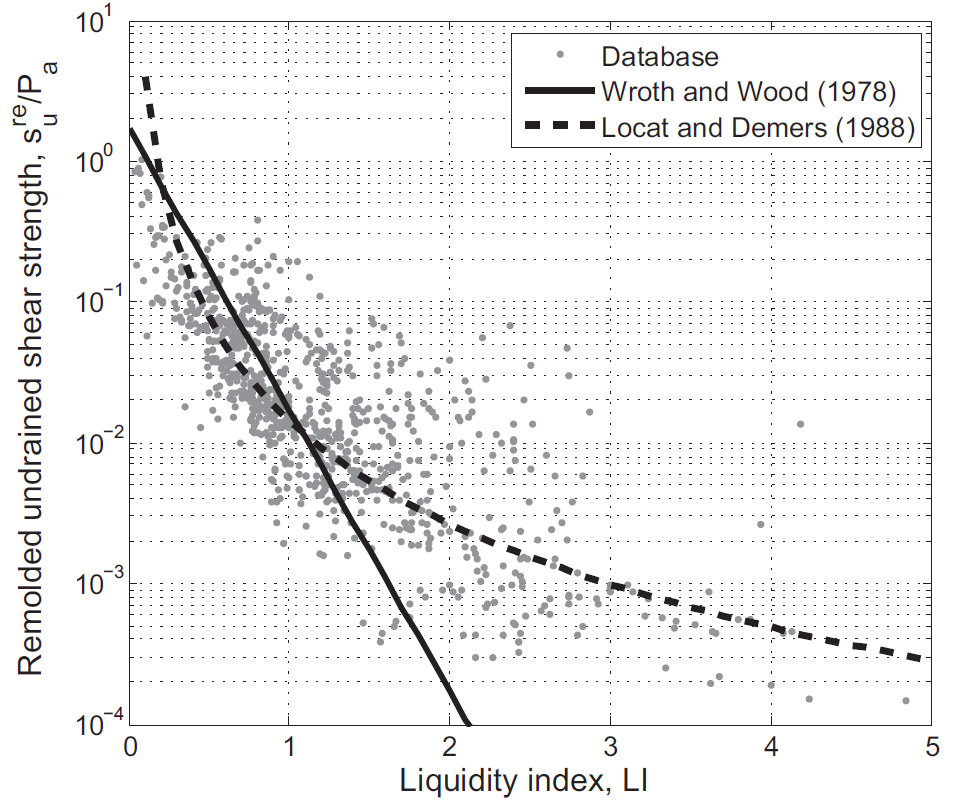
\includegraphics[width=\textwidth]{figures/figure-2.png}
        \caption{$\rm{LI}-(s_u^{re}/P_a)$ models proposed by \citet{Wroth1978137} and \citet{Locat1988799}.}
        \vspace{-5pt}
        \addtocounter{figure}{-1}
        \renewcommand{\figurename}{图}
        \caption{\citet{Wroth1978137}和\citet{Locat1988799}提出的$\rm{LI}-(s_u^{re}/P_a)$模型。}
        \label{figure:2}
        \renewcommand{\figurename}{Figure}
    \end{minipage}
    \begin{minipage}[t]{0.48\textwidth}
        \centering
        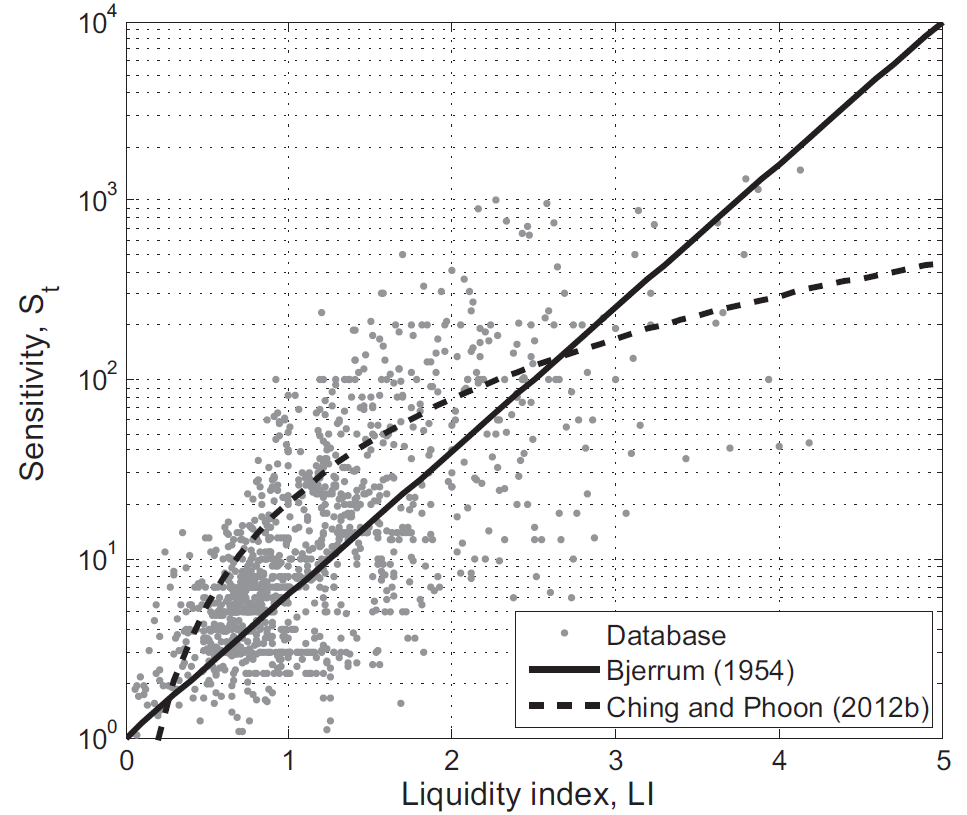
\includegraphics[width=\textwidth]{figures/figure-3.png}
        \caption{$\rm{LI}-S_t$ models proposed by \citet{Bjerrum195449} and \citet{Ching2012522}.}
        \vspace{-5pt}
        \addtocounter{figure}{-1}
        \renewcommand{\figurename}{图}
        \caption{\citet{Bjerrum195449}和\citet{Ching2012522}提出的$\rm{LI}-S_t$模型。}
        \label{figure:3}
        \renewcommand{\figurename}{Figure}
    \end{minipage}
\end{figure*}

\begin{figure*}[!p]
    \centering
    \begin{minipage}[t]{0.48\textwidth}
        \centering
        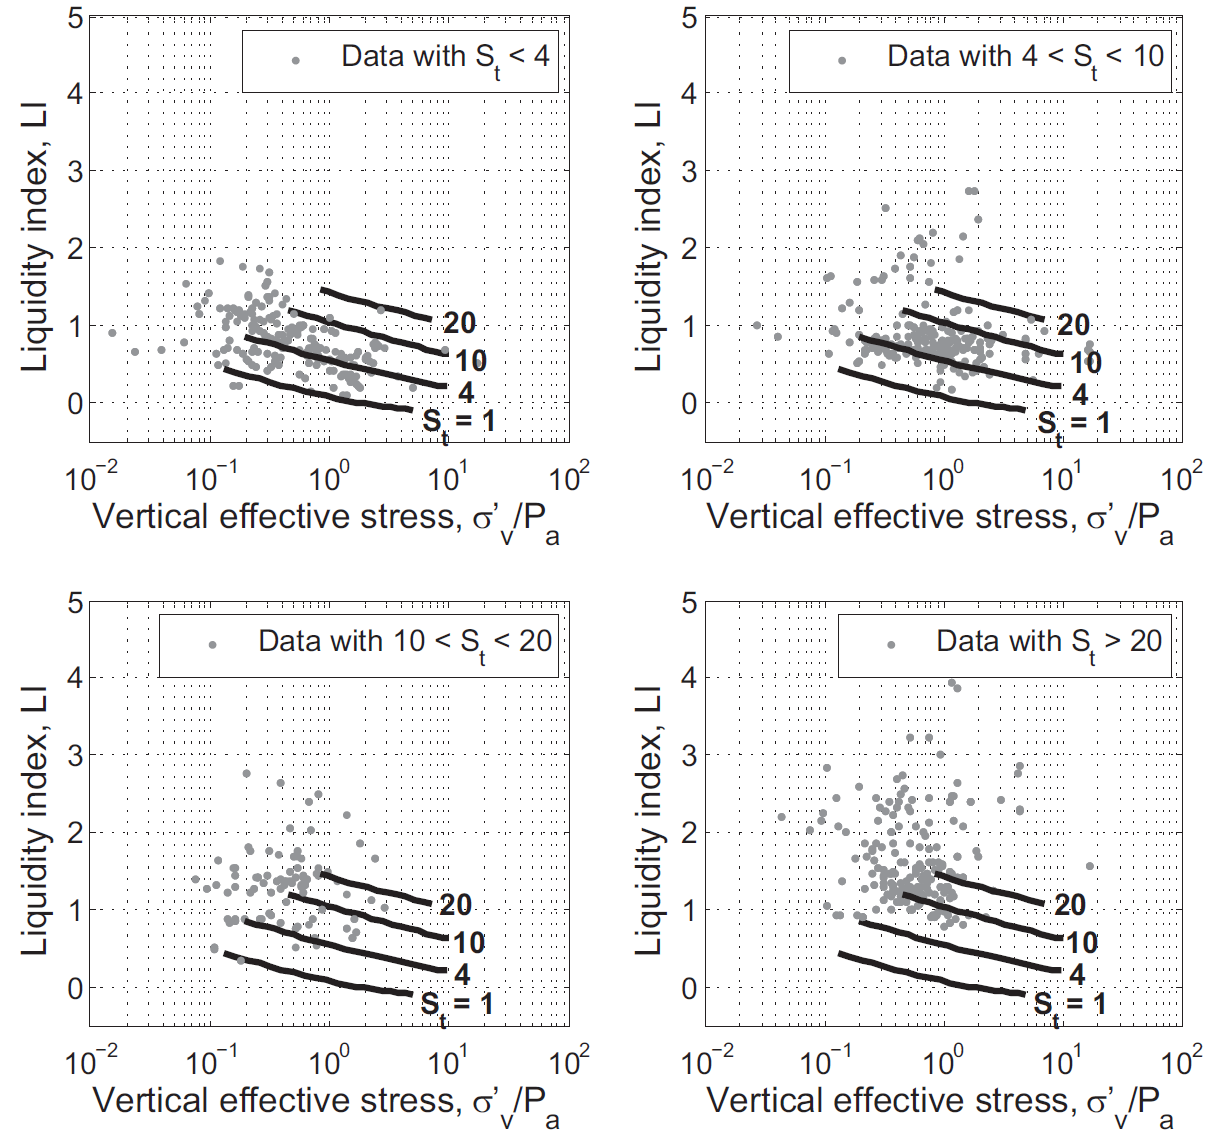
\includegraphics[width=\textwidth]{figures/figure-4.png}
        \caption{$\rm{LI}-(\sigma_v'/P_a)-S_t$ model proposed by \citet{Mitchell1993}.}
        \vspace{-5pt}
        \addtocounter{figure}{-1}
        \renewcommand{\figurename}{图}
        \caption{\citet{Mitchell1993}提出的$\rm{LI}-(\sigma_v'/P_a)-S_t$模型。}
        \label{figure:4}
        \renewcommand{\figurename}{Figure}
    \end{minipage}
    \begin{minipage}[t]{0.48\textwidth}
        \centering
        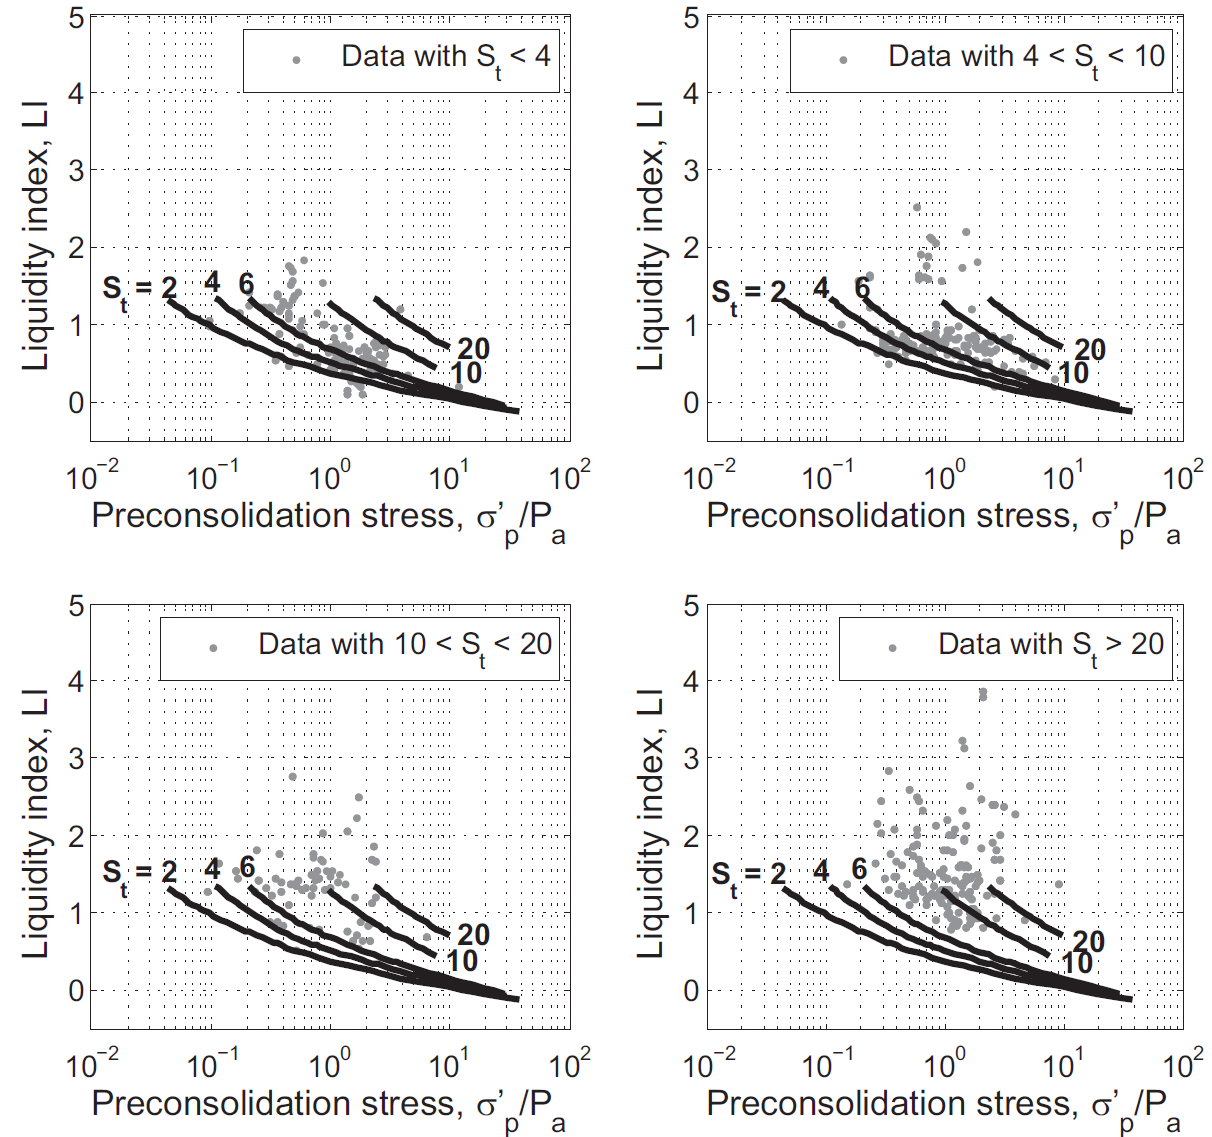
\includegraphics[width=\textwidth]{figures/figure-5.png}
        \caption{$\rm{LI}-(\sigma_p'/P_a)-S_t$ models proposed by \citet{NAVFAC1982}.}
        \vspace{-5pt}
        \addtocounter{figure}{-1}
        \renewcommand{\figurename}{图}
        \caption{\citet{NAVFAC1982}提出的$\rm{LI}-(\sigma_p'/P_a)-S_t$模型。}
        \label{figure:5}
        \renewcommand{\figurename}{Figure}
    \end{minipage}
\end{figure*}

\begin{figure*}[!p]
    \centering
    \begin{minipage}[t]{0.48\textwidth}
        \centering
        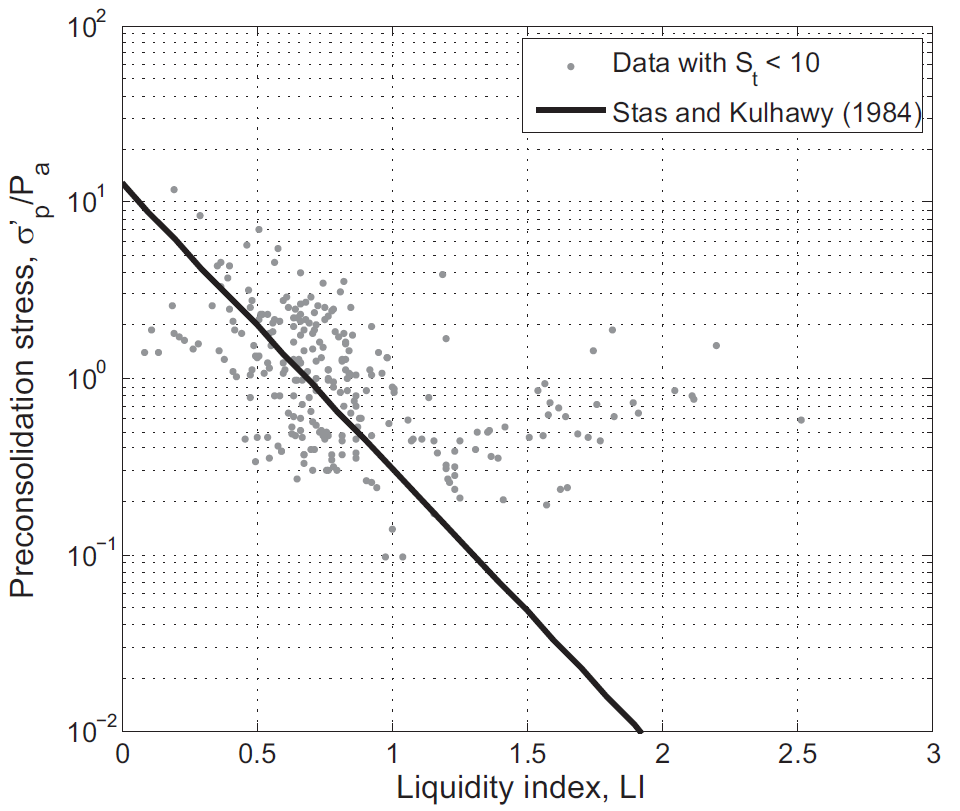
\includegraphics[width=\textwidth]{figures/figure-6.png}
        \caption{$\rm{LI}-(\sigma_p'/P_a)-S_t$ model proposed by \citet{Stas1984}.}
        \vspace{-5pt}
        \addtocounter{figure}{-1}
        \renewcommand{\figurename}{图}
        \caption{\citet{Stas1984}提出的$\rm{LI}-(\sigma_p'/P_a)-S_t$模型。}
        \label{figure:6}
        \renewcommand{\figurename}{Figure}
    \end{minipage}
    \begin{minipage}[t]{0.48\textwidth}
        \centering
        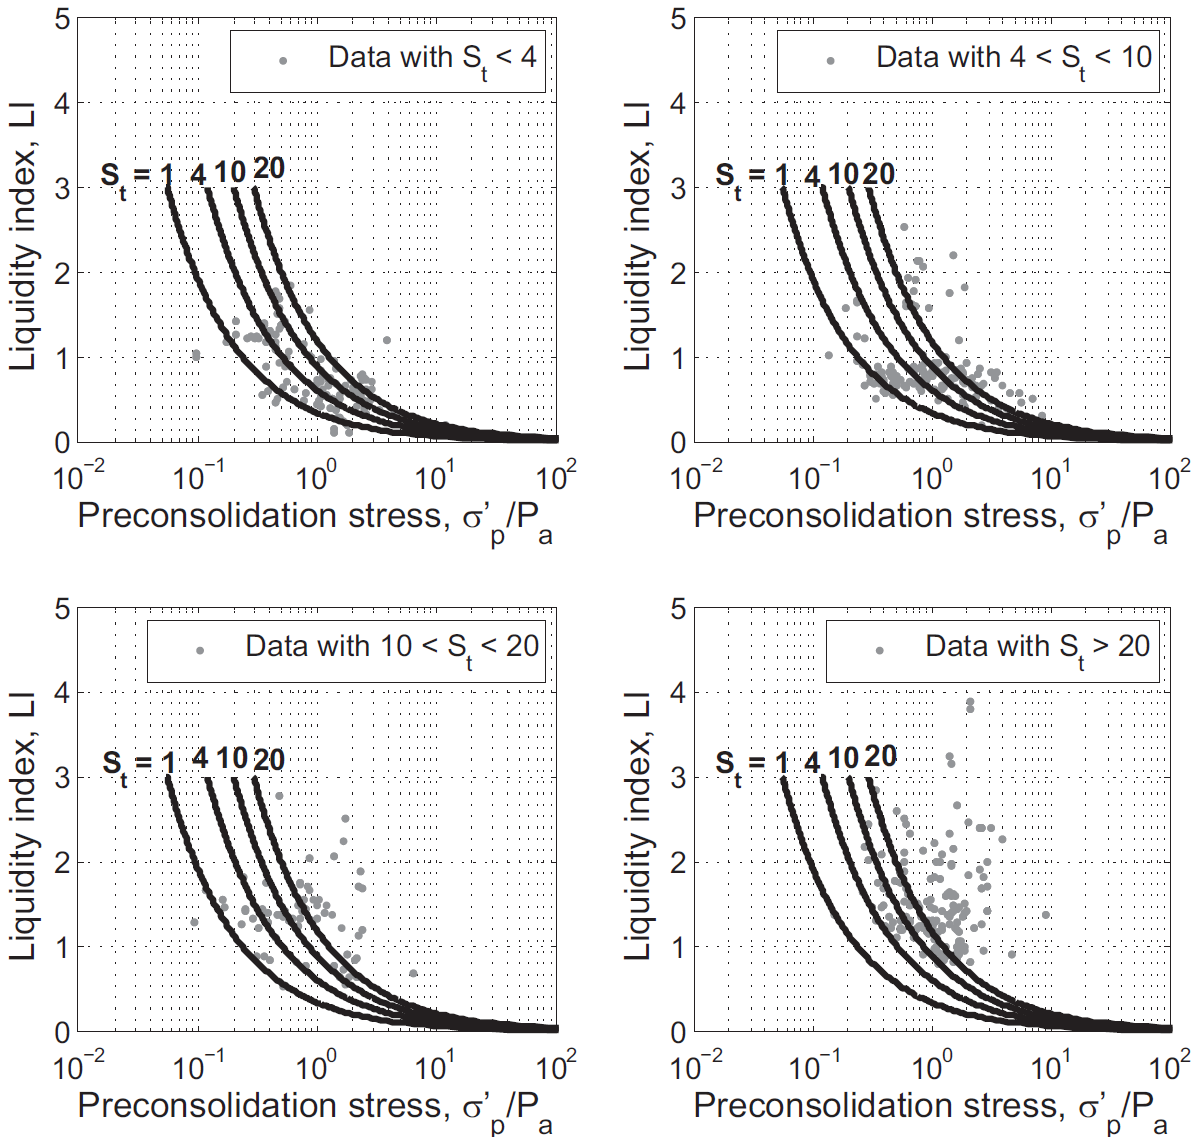
\includegraphics[width=\textwidth]{figures/figure-7.png}
        \caption{$\rm{LI}-(\sigma_p'/P_a)-S_t$ models proposed by \citet{Ching2012522}.}
        \vspace{-5pt}
        \addtocounter{figure}{-1}
        \renewcommand{\figurename}{图}
        \caption{\citet{Ching2012522}提出的$\rm{LI}-(\sigma_p'/P_a)-S_t$模型。}
        \label{figure:7}
        \renewcommand{\figurename}{Figure}
    \end{minipage}
\end{figure*}

\begin{figure*}[!p]
    \centering
    \begin{minipage}[t]{0.48\textwidth}
        \centering
        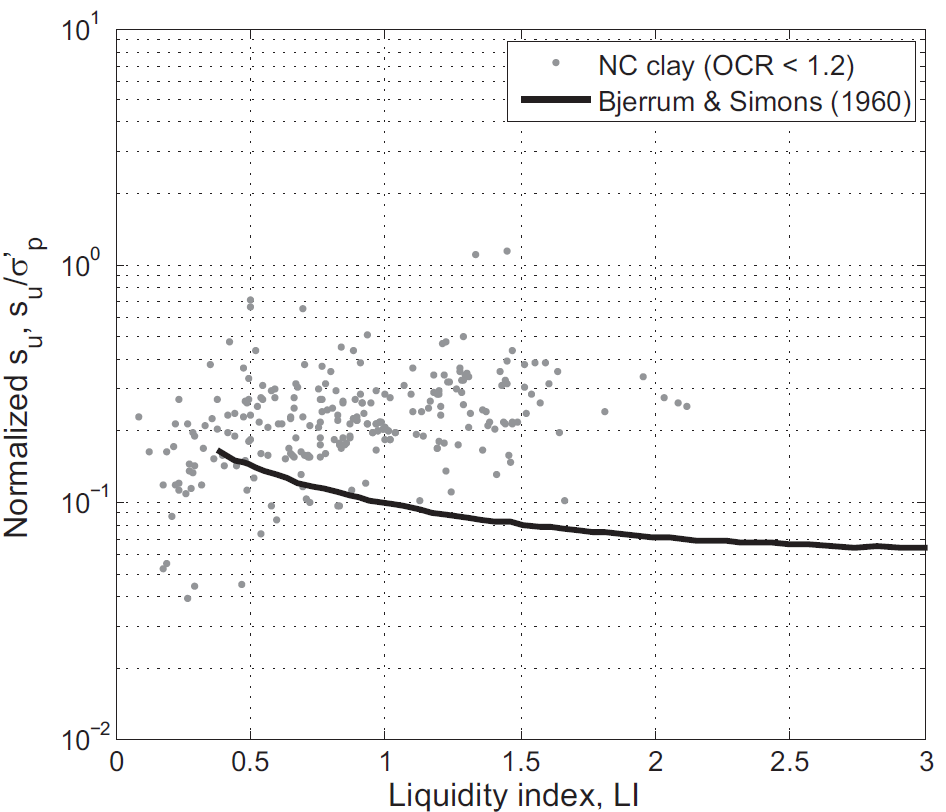
\includegraphics[width=\textwidth]{figures/figure-8.png}
        \caption{$\rm{LI}-(s_u/\sigma_p')$ model proposed by \citet{Bjerrum1960711}.}
        \vspace{-5pt}
        \addtocounter{figure}{-1}
        \renewcommand{\figurename}{图}
        \caption{\citet{Bjerrum1960711}提出的$\rm{LI}-(s_u/\sigma_p')$模型。}
        \label{figure:8}
        \renewcommand{\figurename}{Figure}
    \end{minipage}
    \begin{minipage}[t]{0.48\textwidth}
        \centering
        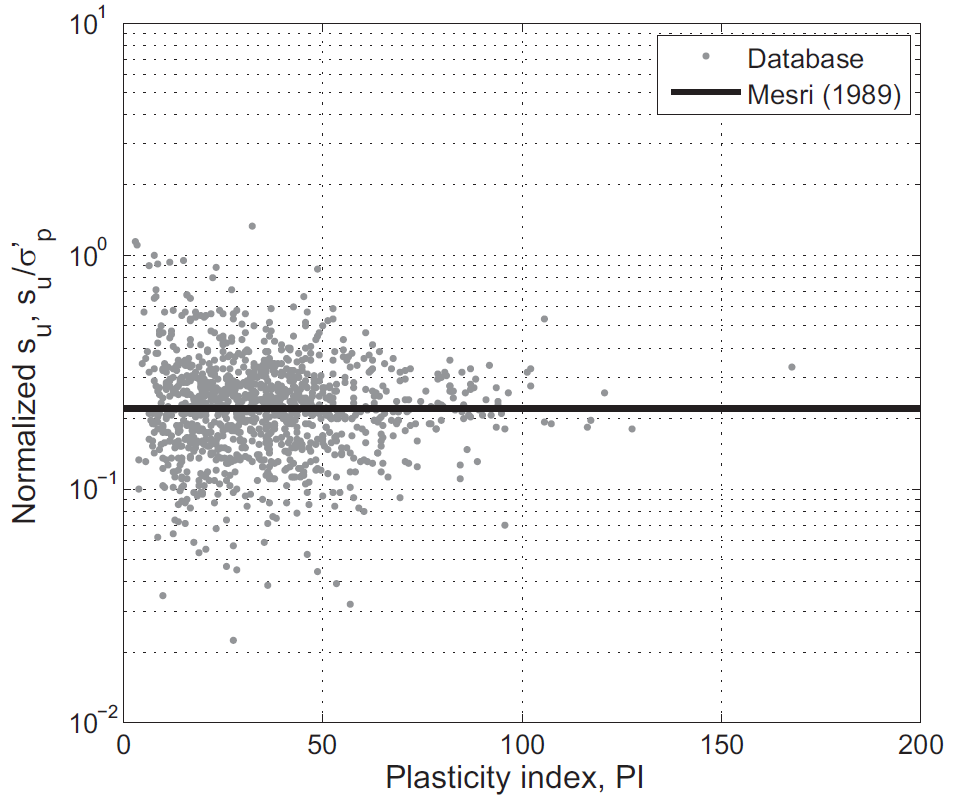
\includegraphics[width=\textwidth]{figures/figure-9.png}
        \caption{$\rm{LI}-(s_u/\sigma_p')$ models proposed by \citet{Mesri1975409, Mesri1989162}.}
        \vspace{-5pt}
        \addtocounter{figure}{-1}
        \renewcommand{\figurename}{图}
        \caption{\citet{Mesri1975409, Mesri1989162}提出的$\rm{LI}-(s_u/\sigma_p')$模型。}
        \label{figure:9}
        \renewcommand{\figurename}{Figure}
    \end{minipage}
\end{figure*}

\begin{figure*}[!p]
    \centering
    \begin{minipage}[t]{0.48\textwidth}
        \centering
        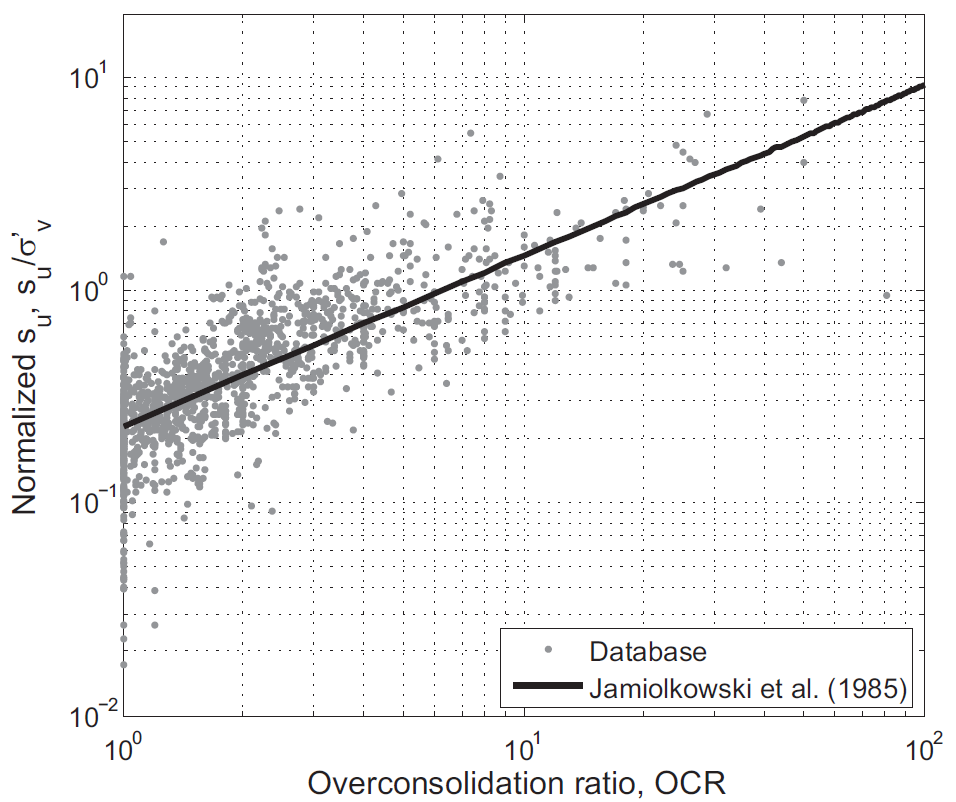
\includegraphics[width=\textwidth]{figures/figure-10.png}
        \caption{$\rm{OCR}-(s_u/\sigma_p')$ model proposed by \citet{Jamiolkowski198557}.}
        \vspace{-5pt}
        \addtocounter{figure}{-1}
        \renewcommand{\figurename}{图}
        \caption{\citet{Jamiolkowski198557}提出的$\rm{OCR}-(s_u/\sigma_p')$模型。}
        \label{figure:10}
        \renewcommand{\figurename}{Figure}
    \end{minipage}
    \begin{minipage}[t]{0.48\textwidth}
        \centering
        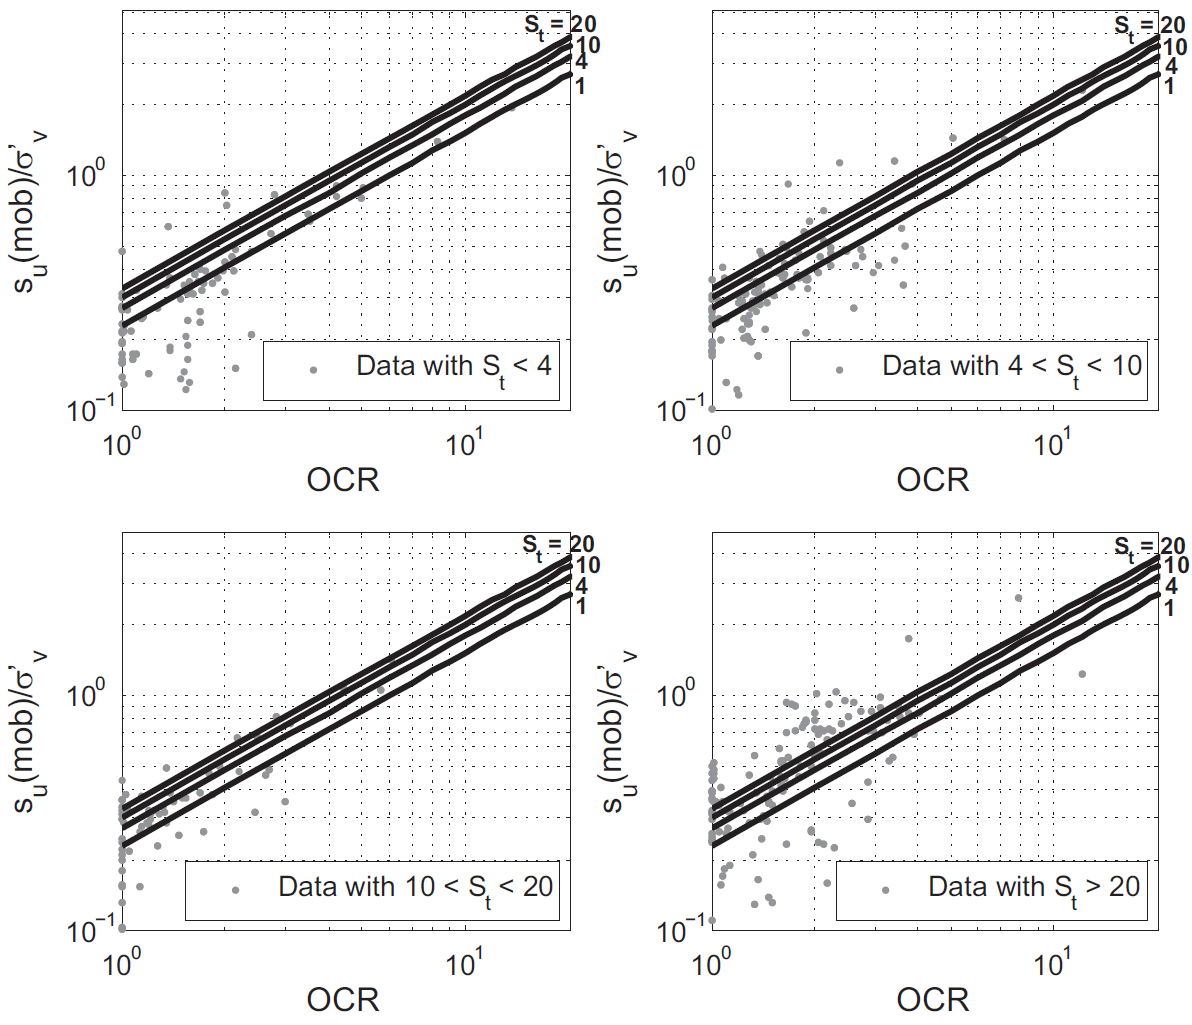
\includegraphics[width=\textwidth]{figures/figure-11.png}
        \caption{$\rm{OCR}-(s_u/\sigma_p')-S_t$ models proposed by \citet{Ching2012522}.}
        \vspace{-5pt}
        \addtocounter{figure}{-1}
        \renewcommand{\figurename}{图}
        \caption{\citet{Ching2012522}提出的$\rm{OCR}-(s_u/\sigma_p')-S_t$模型。}
        \label{figure:11}
        \renewcommand{\figurename}{Figure}
    \end{minipage}
\end{figure*}

\begin{figure*}[!p]
    \centering
    \begin{minipage}[t]{0.48\textwidth}
        \centering
        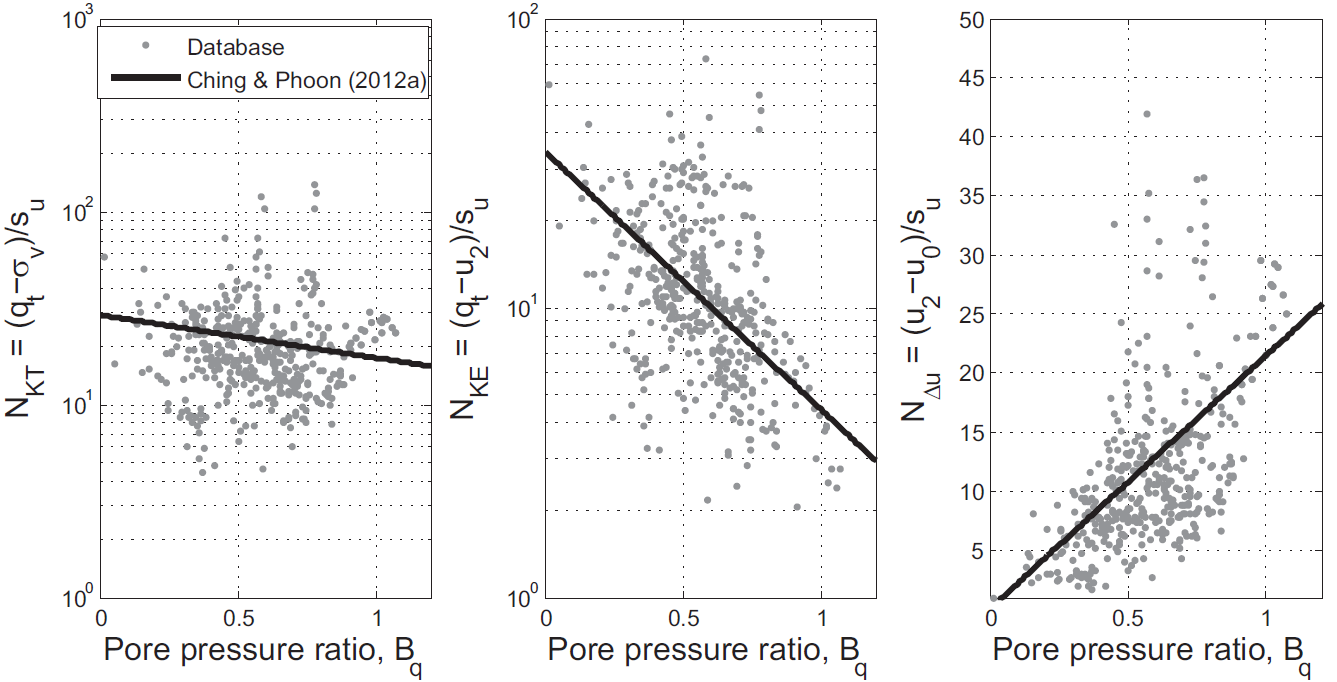
\includegraphics[width=\textwidth]{figures/figure-12.png}
        \caption{$\rm{CPTU}-s_u/\sigma_v'$ model proposed by \citet{Ching2012522}.}
        \vspace{-5pt}
        \addtocounter{figure}{-1}
        \renewcommand{\figurename}{图}
        \caption{\citet{Ching2012522}提出的$\rm{CPTU}-s_u/\sigma_v'$模型。}
        \label{figure:12}
        \renewcommand{\figurename}{Figure}
    \end{minipage}
    \begin{minipage}[t]{0.48\textwidth}
        \centering
        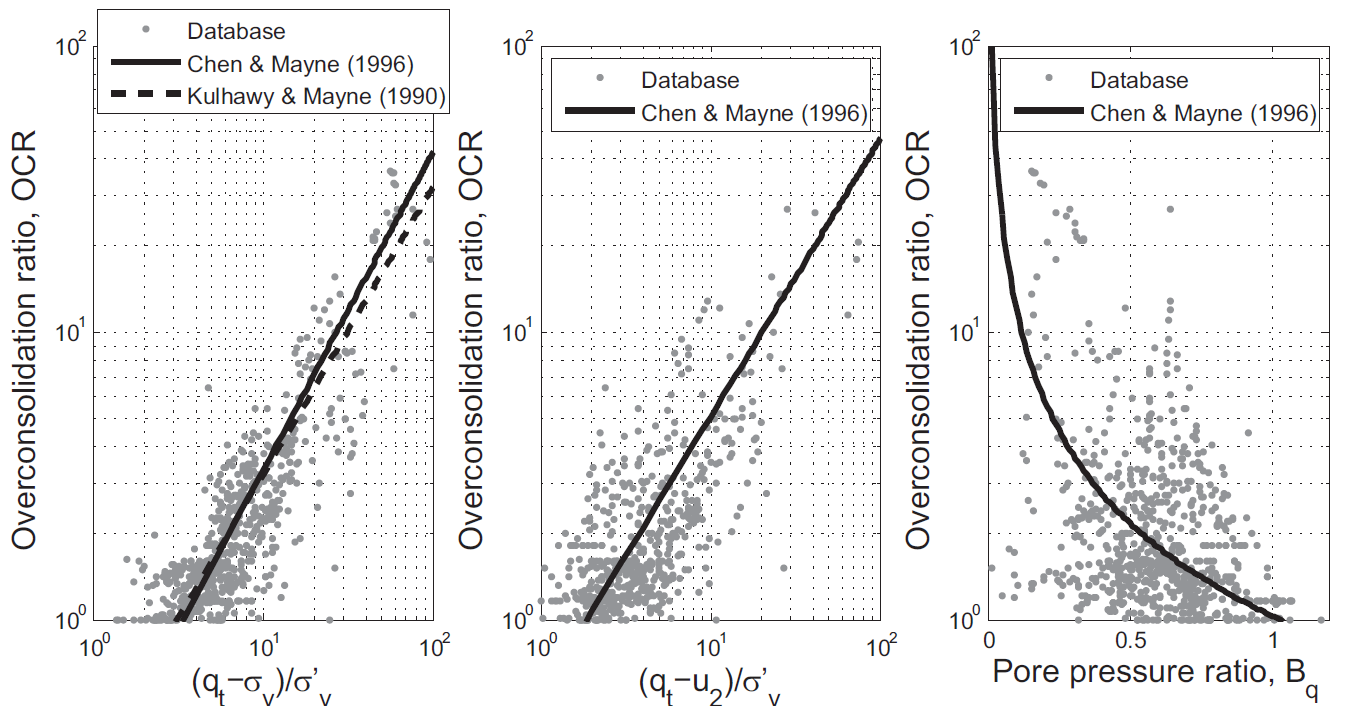
\includegraphics[width=\textwidth]{figures/figure-13.png}
        \caption{CPTU-OCR model proposed by \citet{Chen1996488, Kulhawy1990}.}
        \vspace{-5pt}
        \addtocounter{figure}{-1}
        \renewcommand{\figurename}{图}
        \caption{\citet{Chen1996488, Kulhawy1990}提出的CPTU-OCR模型。}
        \label{figure:13}
        \renewcommand{\figurename}{Figure}
    \end{minipage}
\end{figure*}

\begin{figure*}[!p]
    \centering
    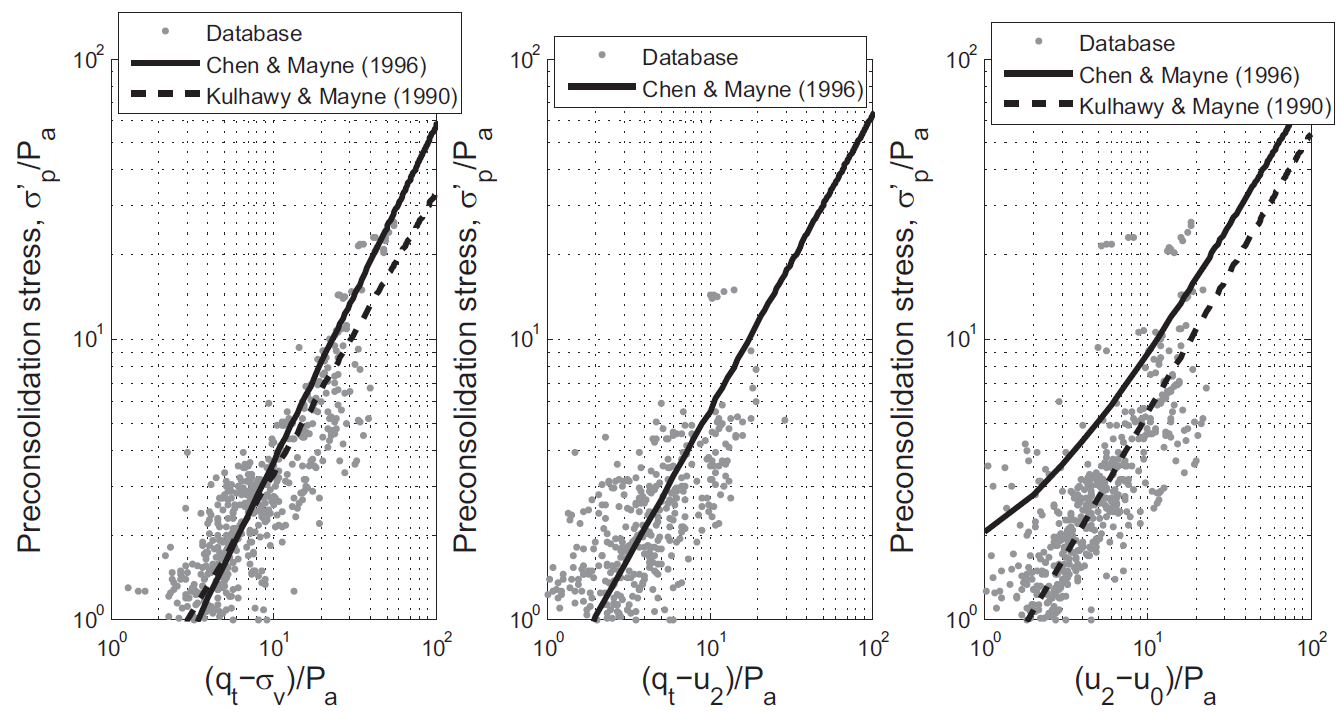
\includegraphics[width=0.5\textwidth]{figures/figure-14.png}
    \caption{$\rm{CPTU}-\sigma_p'/P_a$ model proposed by \citet{Chen1996488, Kulhawy1990}.}
    \vspace{-5pt}
    \addtocounter{figure}{-1}
    \renewcommand{\figurename}{图}
    \caption{\citet{Chen1996488, Kulhawy1990}提出的$\rm{CPTU}-\sigma_p'/P_a$模型。}
    \label{figure:14}
    \renewcommand{\figurename}{Figure}
\end{figure*}

    \ParallelLText
    {
        The comparison results between the transformation models and the database are shown in \autoref{figure:2}–\autoref{figure:14}. For the models with a secondary input parameter St, data points in our database are divided into four groups according to their St values, and four subplots are presented to compare with the transformation models. The four groups are obtained based on St < 4, 4 < St < 10, 10 < St < 20, and St > 20. \autoref{figure:2}~–~\autoref{figure:14} show that the global data follow similar trends to most transformation models reported in the literature. The exceptions are the following six models:

        1. The $\rm{LI}-(s_u^{re}/P_a)$ model proposed by \citet{Wroth1978137}. This model was developed based on the modified Cam Clay model. It provides a reasonable average fit to the data for LI < 1 as shown in \autoref{figure:2}. However, it deviates significantly from the data points in our global database for LI > 1.5.

        2. The $\rm{LI}-(\sigma_v'/P_a)-S_t$ model proposed by \citet{Mitchell1993}. Despite the wide scatter as shown in \autoref{table:4}, there is general agreement between this model and the global data for data points with 4 < St < 20. However, for data with small St values (St < 4) or with large St values (St > 20), the agreement is poor. It is possible that this model was developed with most data points falling between 4 < St < 20. In other words, the empirical support for small and large St values may be weak.

        3. The $\rm{LI}-(\sigma_p'/P_a)-S_t$ model proposed by \citet{NAVFAC1982}. The observations here are similar to those for the Mitchell’s model: there is a reasonably good agreement between the model and the global data for data points with 4 < St < 20 (see \autoref{figure:5}). The agreement is poor outside this range of St. One may venture to guess that the empirical support for small and large St values is also weak for this model.

        4. The $\rm{LI}-(\sigma_p'/P_a)-S_t$ model proposed by \citet{Ching2012522}. The agreement between this model and the global data are reasonable for data points with large St values (St > 20) as shown in \autoref{figure:7}. However, this model does not fit data with small St values (St < 4). This is because the database CLAY/5/345 used to develop this $\rm{LI}-(\sigma_p'/P_a)-S_t$ model contains only structured clays.

        5. $\rm{LI}-(s_u/\sigma_p')$ model proposed by \citet{Bjerrum1960711}. In \autoref{figure:8}, only data points with OCR < 1.2 (nearly NC clays) in the global database are plotted. Nonetheless, the discrepancy between the model and the data is clear. Note that this model was developed based on Norwegian NC clays only. It is most likely that this site-specific model fits to the Norwegian data, but not to the global data from diverse geographic origins.
        
        6. One of the $\rm{CPTU}-(\sigma_p'/P_a)$ models proposed by \citet{Chen1996488} (the third model that relates $\sigma_p'$ to $(u_2-u_0)/P_a$ in \autoref{table:5}). The discrepancy between this model and our global data is apparent. However, the first two models developed by \citet{Chen1996488} (the two models that relate $\sigma_p'/P_a$ to $(q_t-\sigma_v)/P_a$ and $(q_t-u_2)/P_a$) provide reasonable fits to our global data. We are unable to explain this anomaly.
    }
    \ParallelRText
    {
        转换模型与数据库的比较结果如\cnfigureref{figure:2}-\cnfigureref{figure:14}所示。 对于具有辅助输入参数St的模型,我们数据库中的数据点根据其St值分为四组,并提出了四个子图与转换模型进行比较。 根据St < 4,4 <St <10,10 <St <20和St > 20获得这四个组。\cnfigureref{figure:2}–\cnfigureref{figure:14}显示,全球数据遵循与文献中报道的大多数转换模型相似的趋势。 以下六个模型除外:

        1. \citet{Wroth1978137}提出的$\rm{LI}-(s_u^{re}/P_a)$模型。该模型是基于修改后的Cam Clay模型开发的。如\cnfigureref{figure:2}所示,它为LI < 1的数据提供了合理的平均拟合。但是,对于我们的LI > 1.5,它与我们的全局数据库中的数据点有很大的出入。

        2. \citet{Mitchell1993}提出的$\rm{LI}-(\sigma_v'/P_a)-S_t$模型。尽管如\cnfigureref{table:4}所示分散范围很广,但是对于4 <St <20的数据点,该模型与全局数据之间存在普遍共识。但是,对于St值小的(St < 4)或St值大的数据(St > 20),匹配性很差。该模型可能是在大多数数据点落在4 < St < 20之间的情况下开发的。换句话说,对小和大的St值的经验支持可能很弱。

        3. \citet{NAVFAC1982}提出的$\rm{LI}-(\sigma_p'/P_a)-S_t$模型。这里的观察结果与Mitchell模型的观察结果相似:对于4 < St <20的数据点,模型与全局数据之间存在相当好的一致性(见\cnfigureref{figure:5})。在St的这一范围之外,该匹配的效果很差。有人可能会猜测,对于该模型,对于小和大的St值的经验支持也很弱。

        4. \citet{Ching2012522}提出的$\rm{LI}-(\sigma_p'/P_a)-S_t$模型。如\cnfigureref{figure:7}所示,此模型与全局数据之间的一致性对于具有较大St值(St > 20)的数据点是合理的。但是,此模型不适用于具有较小St值(St < 4)的数据。这是因为用于开发此$\rm{LI}-(\sigma_p'/P_a)-S_t$模型的数据库CLAY/5/345仅包含结构化粘土。
        
        5. \citet{Bjerrum1960711}提出的$\rm{LI}-(s_u/\sigma_p')$模型。在\cnfigureref{figure:8}中,仅绘制了全局数据库中OCR < 1.2(接近NC黏土)的数据点。尽管如此,模型和数据之间的差异仍然很明显。请注意,此模型仅基于挪威NC黏土开发。此特定于站点的模型很可能适合挪威的数据,但不适合来自不同地理来源的全球数据。
        
        6. \citet{Chen1996488}提出的$\rm{CPTU}-(\sigma_p'/P_a)$模型之一(\cntableref{table:5}中$\sigma_p'$与$(u_2-u_0)/P_a$相关的第三种模型)。该模型与我们的全局数据之间的差异显而易见。然而,由\citet{Chen1996488}开发的前两个模型($\sigma_p'/P_a$与$(q_t-\sigma_v)/P_a$相关的模型和$(q_t-u_2)/P_a$模型)合理地拟合了我们的全球数据。我们无法解释这种异常。
    }
    \ParallelPar
\end{Parallel}
\section{Biases and uncertainties of the existing transformation models 现有转换模型的偏差和不确定性}

\begin{Parallel}{0.60\textwidth}{}
    \ParallelLText
    {
        The bias factors and coefficients of variation (COVs) of all models with respect to the global database are calibrated, except the three models that are only presented as graphical curves in the literature. The bias factor is denoted by $b$, and the COV is denoted by $\delta$. Basically, $b$ is the sample mean of (actual target value)/(predicted target value) for the global data points, and $\delta$ is the sample COV of (actual target value)/(predicted target value). For instance, for the $\rm{LI}-(s_u^{re}/P_a)$ model proposed by \citet{Locat1988799}, the actual target value is the $s_u^{re}/P_a$ value in the global database, and the predicted target value is $0.0144\rm{LI}^{-2.44}$. For each data point with simultaneous knowledge of $(\rm{LI},~s_u^{re})$, (actual target value)/(predicted target value) = $(s_u^{re}/P_a)/(0.0144\rm{LI}^{-2.44})$ can be computed. The histogram of the ratio $(s_u^{re}/P_a)/(0.0144\rm{LI}^{-2.44})$ is plotted in Fig. \ref{figure:15}. The sample mean of this ratio is equation to 1.92, which is equation to $b$.The sample COV of this ratio is 1.25, which is  equation to $\delta$. To be specific,
    }
    \ParallelRText
    {
        本文校正了所有模型相对于全局数据库的偏差因子和变异系数(COV),除了在文献中仅以图形曲线形式表示的三个模型外。 偏置因子用$b$表示,COV用$\delta$表示。 基本上,$b$是全局数据点的(实际目标值)/(预测目标值)的样本均值,并且$\delta$是(实际目标值)/(预测目标值)的样本COV。 例如,对于\citet{Locat1988799}提出的$\rm{LI}-(s_u^{re}/P_a)$模型,实际目标值为全球数据库中的$s_u^{re}/P_a$值,而预测目标值为$0.0144\rm{LI}^{-2.44}$。 对于同时了解$(\rm{LI},~s_u^{re})$的每个数据点,可以计算(实际目标值)/(预测目标值)= $(s_u^{re}/P_a)/(0.0144\rm{LI}^{-2.44})$。 比值的直方图$(s_u^{re}/P_a)/(0.0144\rm{LI}^{-2.44})$绘制在图\ref{figure:15}中。该比值的样本平均值等于1.92,等于$b$。此比率的样本COV为1.25,等于$\delta$。 再具体一点,
        
    }
    \ParallelPar
    \begin{align}
        \rm{Actual~ target~value = predicted~target~value\times{}b\times{}\delta}
        \label{equation:1}
    \end{align}
    \begin{figure}[!htb]
    \centering
    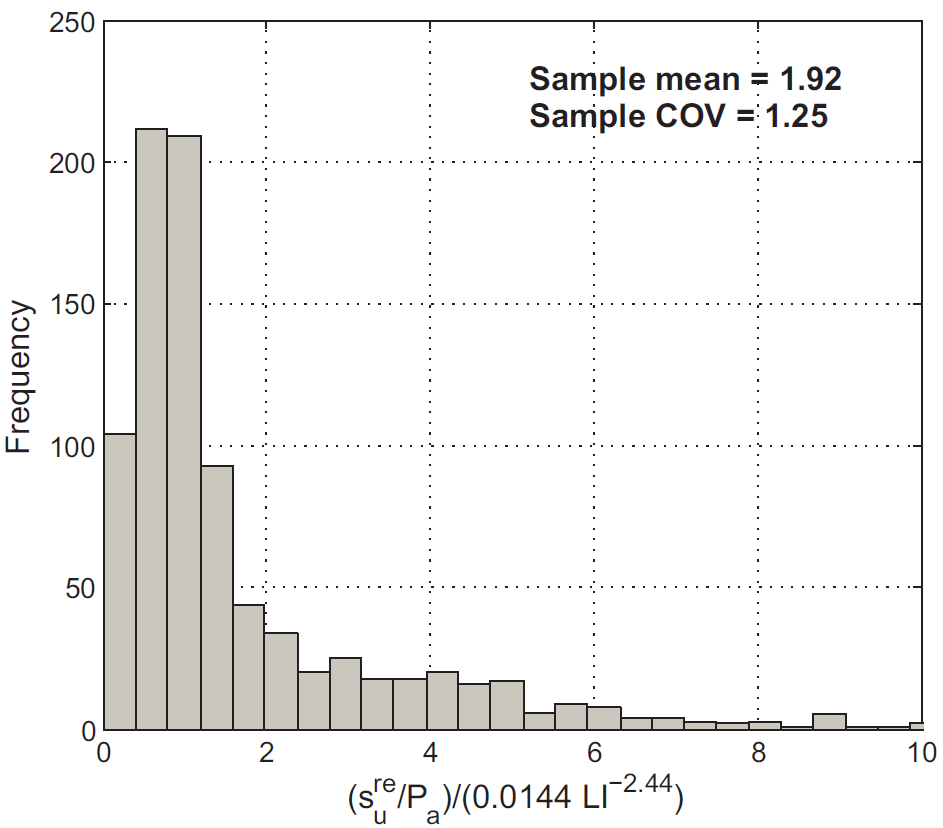
\includegraphics[width=0.5\textwidth]{figures/figure-15.png}
    \caption{Histogram of $(s_u^{re}/P_a)/(0.0144\rm{LI}^{-2.44})$.}
    \addtocounter{figure}{-1}
    \vspace{-5pt}
    \renewcommand{\figurename}{图}
    \caption{$(s_u^{re}/P_a)/(0.0144\rm{LI}^{-2.44})$的直方图。}
    \renewcommand{\figurename}{Figure}
    \label{figure:15}
\end{figure}
    \ParallelLText
    {
        where b is the bias factor ($b$ = 1 means unbiased) and $\epsilon$ is the variability term with mean = 1 and COV = $\delta$. If $\delta = 0$, there is no data scatter about the transformation model, i.e., the prediction is single-valued or deterministic, rather than a distribution. The $\rm{LI}-(s_u^{re}/P_a)$ model proposed by \citet{Locat1988799} is biased because the bias factor ($b$) is around 1.92, and the COV of this model is around 1.25. This model basically underpredicts the actual value by a factor of about 2 (conservative model). The uncertainty underlying this prediction when it is made to cover the wide range of conditions in the global database is considerable given that the COV exceeds 100$\%$. The calibrated bias factors and COVs for all models are shown in the last two columns of Table \ref{table:5}. The number of data points “$n$” used for each calibration is listed in the table.
    }
    \ParallelRText
    {
        式中$b$是偏差因子($b = 1$表示无偏),$\epsilon$是均值= 1且COV = $ \delta $的可变项。 如果$ \delta = 0 $,则没有关于转换模型的数据分散,即预测是单值或确定性的,而不是某种分布。 \citet{Locat1988799}提出的$\rm{LI}-(s_u^{re}/P_a)$模型是有偏差的,因为偏差因子($b$)约为1.92,而该模型的COV约为1.25。 该模型基本上将实际值低估了约2倍(保守模型)。 考虑到COV超过100%,当预测覆盖全球数据库中的广泛条件时,这种不确定性是相当大的。 表\ref{table:5}的最后两列显示了所有模型的校准偏差因子和COV。表中列出了每次校准使用的数据点“$n$”的数量。
    }
    \ParallelPar
    \ParallelLText
    {
        It is evident that models published in more recent studies, such as citet{Kulhawy1990}, \citet{Chen1996488}, and \citet{Ching201252, Ching2012522} mostly have bias factors $b\approx{}1$ (less biased). These recent studies compiled fairly large databases as well. It is also evident that the COVs ($\delta$) calibrated by the global database in this study are typically higher than those reported in the literature (see the numbers in the parentheses in the rightmost column in Table \ref{table:5}). The exceptions are the $\rm{LI}–S_t$, $\rm{LI}-(\sigma_p'/P_a)-S_t$ and $\rm{OCR}-(s_u/\sigma_v')-S_t$ models developed in \citet{Ching2012522}: COVs for these three models are close to those reported in \citet{Ching2012522}. The statistics of the database used by \citet{Ching2012522} are given in the “Remarks” column in Table \ref{table:5}. 
    }
    \ParallelRText
    {
        显然,在最近的研究中发表的模型,例如\citet{Kulhawy1990},\citet{Chen1996488}以及\citet{Ching201252, Ching2012522},大多具有偏差因子$b\approx{}1$(偏差较小)。 这些最近的研究也汇编了相当大的数据库。 同样明显的是,这项研究中由全球数据库校准的COV($\delta$)通常高于文献报道的COV(请参见表\ref{table:5}最右栏中的括号中的数字)。 \citet{Ching2012522}开发的$\rm{LI}–S_t$,$\rm{LI}-(\sigma_p'/P_a)-S_t$和$\rm{OCR}-(s_u/\sigma_v')-S_t$模型除外:这三个模型的COV接近\citet{Ching2012522}中报道的那些。\citet{Ching2012522}使用的数据库的统计信息在表\ref{table:5}的“备注”列中给出。
    }
    \ParallelPar
    \ParallelLText
    {
        The bias factors in Table \ref{table:5} still deviate somewhat from unity for two possible reasons:

        1. The bias factors in Table \ref{table:5} are calibrated using the global database in this study that contains broader types of clays, typically broader than the databases used to develop the transformation models in the literature. For instance, \citet{Ching2012522} only considered structured clays.

        2. All $s_u$ data points in the global database are converted to $s_u(\rm{mob})$ (see Table \ref{table:2}). Such a conversion step may introduce an extra bias.
    }
    \ParallelRText
    {
        表\ref{table:5}中的偏差因子仍因某些可能的原因而偏离统一性:

        1. 使用本研究中的全球数据库对表\ref{table:5}中的偏差因子进行校准,该数据库包含更广泛的黏土类型,通常比文献中用于开发转化模型的数据库更广泛。 例如,\citet{Ching2012522}仅考虑结构化黏土。
        
        2. 全局数据库中的所有$s_u$数据点都将转换为$s_u(\rm{mob})$(请参见表\ref{table:2})。 这样的转换步骤可能会引入额外的偏差。
    }
    \ParallelPar
    \ParallelLText
    {
        The COVs in Table \ref{table:5} are typically larger than those reported in the literature for three possible reasons:

        1. These COVs are calibrated using the global database that contains broader types of clays.

        2. The conversion of the $s_u$ data points to a reference strength, $s_u(\rm{mob})$, would introduce transformation uncertainty. It is noteworthy that the COVs can be even larger without this conversion, because su varies significantly with the test type \citep{Ladd1977421}.
        
        3. The COVs summarized in \citet{Ching201252} for the $\rm{CPTU}-(s_u/\sigma_v')$ transformation models do not include measurement errors.
    }
    \ParallelRText
    {
        由于以下三种可能的原因,表\ref{table:5}中的COV通常大于文献报道的COV:

        1. 使用包含更广泛类型的黏土的全球数据库对这些COV进行校准。

        2. 将$s_u$数据点转换为参考强度$s_u(\rm{mob})$,将引入转换不确定性。 值得注意的是,如果不进行这种转换,COV可能会更大,因为su随测试类型而变化很大\citep{Ladd1977421}。
       
        3. \citet{Ching201252}中针对$\rm{CPTU}-(s_u/\sigma_v')$转换模型总结的COV不包括测量误差。
    }
    \ParallelPar
    \ParallelLText
    {
        By definition, the models calibrated by the global database are unbiased with respect to the global database in this study. For instance, for the $\rm{LI}-s_u^{re}/P_a$ model by \cite{Locat1988799}, the predicted value for $s_u^{re}/P_a$ is $0.0144\rm{LI}^{-2.44}$. This model has a bias factor $b = 1.92$, calibrated by the global database. As a result, the calibrated model $s_u^{re}/P_a\approx{}b(0.0144)\rm{LI}^{-2.44}=1.92(0.0144)\rm{LI}^{-2.44}$ is an “unbiased prediction” with respect to the global database. This means that this calibrated model can capture the mean trend of the global database, and the calibrated COV can adequately capture the data scatter around the mean trend. However, the COV is typically quite large to capture the data scatter. In the next section, the possibility of incorporating secondary input parameters to reduce the COV is addressed.
    }
    \ParallelRText
    {
        根据定义,在本研究中,由全局数据库校准的模型相对于全局数据库没有偏见。 例如,对于\cite{Locat1988799}的$\rm{LI}-s_u^{re}/P_a$模型,$s_u^{re}/P_a$的预测值为$0.0144\rm{LI}^{-2.44}$。 该模型的偏差因子$b = 1.92$,已通过全局数据库进行了校准。 结果,校准后的模型$s_u^{re}/P_a\approx{}b(0.0144)\rm{LI}^{-2.44}=1.92(0.0144)\rm{LI}^{-2.44}$对于全局数据库而言是“无偏预测”。 这意味着该校准模型可以捕获全局数据库的平均趋势,并且校准COV可以充分捕获平均趋势周围的数据散布。 但是,COV通常很大以捕获数据散布。 在下一节中,讨论了合并次级输入参数以降低COV的可能性。
    }
\end{Parallel}
\section{Secondary input parameters 辅助输入参数}

\begin{Parallel}{0.60\textwidth}{}
    \ParallelLText
    {
        A possible reason for the significant data scatter around the mean trend is that additional explanatory variables are not incorporated into the transformation model. As a result, the variation in these hidden explanatory variables, which is inevitable in a database, is added to the transformation uncertainty. A good example is the $\rm{OCR}-(s_u/\sigma_v')$ model by \citet{Jamiolkowski198557}. The COV with respect to the global database is 0.53 for this model (see Table \ref{table:5}). This means that the standard deviation of the data scatter is about 53$\%$ of the mean trend. A possible hidden explanatory variable is the sensitivity $S_t$ — it is known that the “stress history and normalized soil engineering properties” SHANSEP parameters for sensitive (structured) clays are different from those for insensitive clays. In fact, by incorporating $S_t$ as a secondary input parameter, the $\rm{OCR}-(s_u/\sigma_v')-S_t$ model by \cite{Ching2012522}carries a significantly smaller COV of 0.34 (see Table \ref{table:5}). It is widely known that parameters such as PI and $S_t$ can be applied as secondary explanatory variables for some correlations. It is of interest to see whether the incorporation of these secondary input parameters can reduce COV significantly. If the COV reduction is significant, it is of interest to re-calibrate the transformation models to further update the bias factors and the COVs in Table \ref{table:5}. This is the main objective of this section.
    }
    \ParallelRText
    {
        围绕平均趋势出现大量数据分散的可能原因是,其他解释变量未合并到转换模型中。结果,这些隐藏的解释变量的变化(这在数据库中是不可避免的)被添加到变换不确定性中。一个很好的例子是\citet{Jamiolkowski198557}的$\rm{OCR}-(s_u/\sigma_v')$模型。对于此模型,相对于全局数据库的COV为0.53(请参见表\ref{table:5})。这意味着数据散布的标准偏差约为平均趋势的53$\%$。可能的隐藏解释变量是敏感度$S_t$ - 已知敏感(结构化)黏土的“应力历史和规范化的土壤工程特性” SHANSEP参数与不敏感黏土的参数不同。实际上,通过将$S_t$作为次要输入参数,\cite{Ching2012522}的$\rm{OCR}-(s_u/\sigma_v')-S_t$模型携带的COV值要小得多,为0.34(参见表\ref{table:5})。众所周知,诸如PI和$S_t$之类的参数可以用作某些相关性的次要解释变量。有趣的是,这些辅助输入参数的合并是否可以显着降低COV。如果COV降低很大,则需要重新校准转换模型以进一步更新表\ref{table:5}中的偏置因子和COV。这是本节的主要目标。
    }
\end{Parallel}


\Paragraph{Correlation between $\epsilon$ and $(\rm{PI}, S_t)$ $\epsilon$与$(\rm{PI}, S_t)$之间的相关性}

\begin{Parallel}{0.60\textwidth}{}
    \ParallelLText
    {
        Let us recall from eq. (\ref{equation:1}) that the variability term $\epsilon$ for a  transformation model can be expressed as
    }
    \ParallelRText
    {
        让我们从等式(\ref{equation:1})回忆,转换模型的可变性项$\epsilon$可以表示为
    }
    \ParallelPar
    \begin{align}
        \epsilon=\dfrac{\rm{actual~target~value}}{b\times{}\rm{predicted~target~value}}=\dfrac{\rm{actual~target~value}}{\rm{unbiased~prediction}}
        \label{equation:2}
    \end{align}
    \ParallelLText
    {
        where the unbiased prediction = $b\times$ predicted target value. The variability term epsilou quantifies the deviation between the actual value and the unbiased prediction. It has mean value of 1 and COV equation to the calibrated COV (delta). Equivalently
    }
    \ParallelRText
    {
        其中无偏预测 = $b\times$预测目标值。 可变性项$\varepsilon$量化了实际值和无偏预测之间的偏差。它的平均值为1,且COV等于校准的COV($\delta$)。等效地,
    }
    \ParallelPar
    \begin{align}
        \ln(\varepsilon)=\ln(\rm{actual~target~value})-\ln({\rm{unbiased~prediction}})
        \label{equation:3}
    \end{align}
    \ParallelLText
    {
        In essence, $\ln(\varepsilon)$ is the component that cannot be explained away by the primary input parameter. More precisely, $\ln(\varepsilon)$ should be uncorrelated to the primary input parameter. The reason why the natural logarithm is taken will be explained later. For instance, $\ln(\varepsilon)$ for the $\rm{OCR}-(s_u/\sigma_v')$ model proposed by \citet{Jamiolkowski198557} is indeed nearly uncorrelated to the primary input parameter $\ln(\rm{OCR})$, shown in Fig. \ref{figure:16}a. Incidentally, the correlation between $\ln(\varepsilon)$ and $\ln(\rm{PI})$ is also nearly zero (Fig. \ref{figure:16}b). However, $\ln(\varepsilon)$ and $\ln(S_t)$ show some slight positive correlation (Fig. \ref{figure:16}c). In this case, it may be possible to adopt St as the secondary input parameter for Jamiolkowski et al.’s model to reduce its COV.
    }
    \ParallelRText
    {
        本质上,$\ln(\varepsilon)$是无法由主输入参数解释的成分。 更准确地说,$\ln(\varepsilon)$应该与主要输入参数不相关。 取自然对数的原因将在后面说明。 例如,\citet{Jamiolkowski198557}提出的$\rm{OCR}-(s_u/\sigma_v')$模型的$\ln(\varepsilon)$的确与图\ref{figure:16}a所示的主要输入参数$\ln(\rm{OCR})$几乎不相关。 顺便提及,$\ln(\varepsilon)$和$\ln(\rm{PI})$之间的相关性也几乎为零(图\ref{figure:16}b)。 但是,$\ln(\varepsilon)$和$\ln(S_t)$表现出一些轻微的正相关(图\ref{figure:16}c)。 在这种情况下,有可能采用$S_t$作为Jamiolkowski等人模型的辅助输入参数,以降低其COV。
    }
    \ParallelPar
    \begin{figure}[!htb]
    \centering
    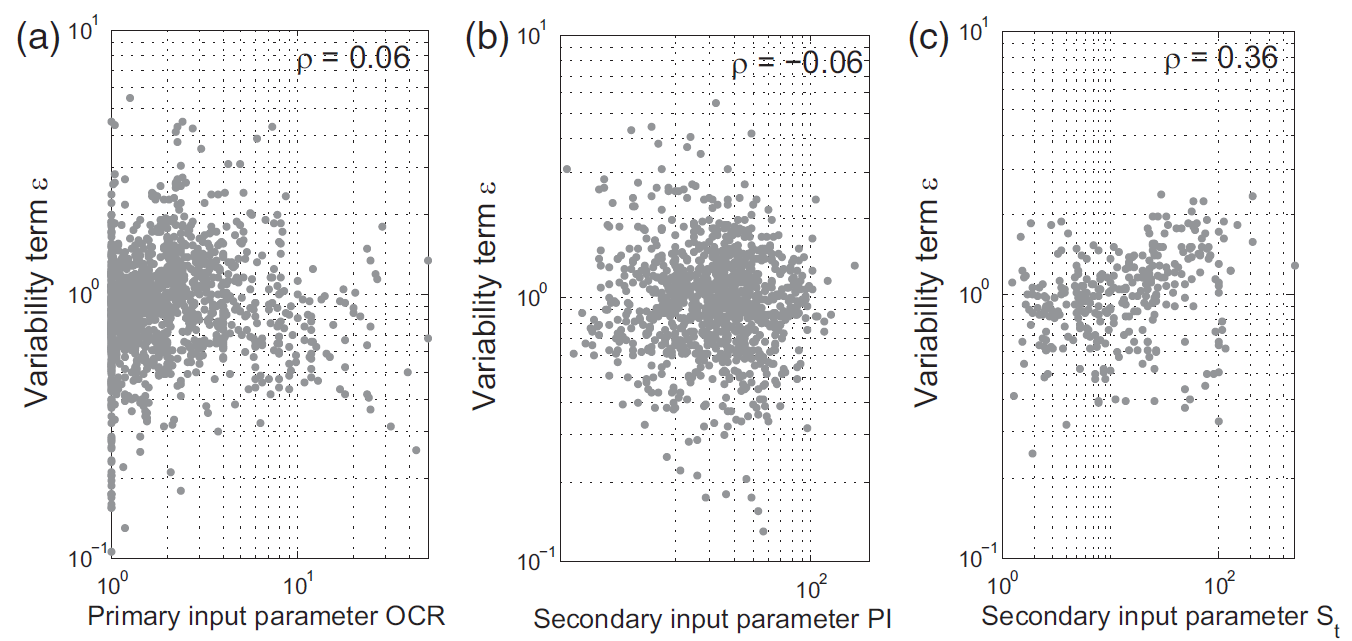
\includegraphics[width=0.7\textwidth]{figures/figure-16.png}
    \caption{(a) $\ln(\varepsilon)–\ln(\rm{OCR})$, (b) $\ln(\varepsilon)–\ln(\rm{PI})$, and (c) $\ln(\varepsilon)–\ln(S_t)$ plots for the model proposed by \citet{Jamiolkowski198557}. $\rho$, correlation coefficient.}
    \addtocounter{figure}{-1}
    \vspace{-5pt}
    \renewcommand{\figurename}{图}
    \caption{(a) $\ln(\varepsilon)–\ln(\rm{OCR})$, (b) $\ln(\varepsilon)–\ln(\rm{PI})$, and (c) $\ln(\varepsilon)–\ln(S_t)$ \citet{Jamiolkowski198557}提出的模型的图解。 $\rho$,相关系数。}
    \renewcommand{\figurename}{Figure}
    \label{figure:16}
\end{figure}
    \ParallelLText
    {
        In this section, the correlation between $\ln(\epsilon)$ and the natural logarithm of the secondary input parameter (PI or $S_t$) will be  studied. The correlation with respect to $\ln(\rm{PI})$ will be studied for all models except the $\rm{PI}-(s_u/\sigma_p')$ model proposed by \citet{Mesri1975409, Mesri1989162}, because PI is already the primary input parameter. Similarly, the correlation with respect to $\ln(S_t)$ will not be studied for models whose primary inputs already involve $S_t$. The correlation with respect to $\ln(S_t)$ will not be studied for models whose target is $s_u^{re}$, because soil structure is supposed to be destroyed in the  remoulded state and hence, it does not make much sense to infer $s_u^{re}$ using $S_t$.
    }
    \ParallelRText
    {
        在本节中,将研究$\ln(\epsilon)$与辅助输入参数(PI或$S_t$)的自然对数之间的相关性。 因为PI已经是主要的输入参数,所以将研究除\citet{Mesri1975409, Mesri1989162}提出的$\rm{PI}-(s_u/\sigma_p')$模型以外的所有模型与$\ln(\rm{PI})$的相关性。 同样,对于主要输入已经包含$S_t$的模型,将不会研究与$\ln(S_t)$的相关性。对于目标为$s_u^{re}$的模型,将不会研究与$\ln(S_t)$的相关性,因为应该在重塑状态下破坏土壤结构,因此使用$S_t$推断$s_u^{re}$没有太大意义。
    }
    \ParallelPar
    \ParallelLText
    {
        The correlation between $\ln(\epsilon)$ and the natural logarithm of the secondary input parameter (PI or $S_t$) is quantified by the Pearson product moment correlation coefficient ($\rho$). The correlation coefficient for the $\ln(\epsilon)-\ln(\rm{PI})$ and $\ln(\epsilon)-\ln(S_t)$ correlations are shown in Table 6. The parameter n shown in Table 6 is the number of data points used to estimate each correlation. It is clear that the $\ln(\epsilon)-\ln(\rm{PI})$ data points are abundant ($n$ > 300), whereas the $\ln(\epsilon)-\ln(S_t)$ data points are less abundant. It is also evident that the $\ln(\epsilon)-\ln(S_t)$ correlations seem stronger ($\rho$ is farther away from zero) than the $\ln(\epsilon)-\ln(\rm{PI})$ correlations.
    }
    \ParallelRText
    {
        $\ln(\epsilon)$和辅助输入参数(PI或$S_t$)的自然对数之间的相关性通过皮尔逊乘积矩相关系数($\rho$)进行量化。 $\ln(\epsilon)-\ln(\rm{PI})$和 $\ln(\epsilon)-\ln(S_t)$相关性的相关系数如表\ref{table:6}所示。表\ref{table:6}中所示的参数$n$是用于估计每个相关性的数据点数。 显然,$\ln(\epsilon)-\ln(\rm{PI})$数据点数量丰富($n$ > 300),而$\ln(\epsilon)-\ln(S_t)$数据点数量较少。 同样明显的是,$\ln(\epsilon)-\ln(S_t)$相关性似乎比$\ln(\epsilon)-\ln(\rm{PI})$相关性更强($\rho$离零更远)。
    }
    \ParallelPar
    \newcommand{\RelationshipA}{$\rm{LI}-s_u^{re}/P_a$}
\newcommand{\RelationshipB}{$\rm{LI}-S_t$}
\newcommand{\RelationshipC}{$\rm{LI}-\sigma_p'/P_a-S_t$}
\newcommand{\RelationshipD}{$\rm{PI}-s_u/\sigma_p'$}
\newcommand{\RelationshipE}{$\rm{OCR}-s_u/\sigma_p'$}
\newcommand{\RelationshipF}{$\rm{OCR}-s_u/\sigma_p'-S_t$}
\newcommand{\RelationshipG}{$\rm{CPTU}-s_u/\sigma_p'$}
\newcommand{\RelationshipH}{$\rm{CPTU}-\rm{OCR}$}
\newcommand{\RelationshipI}{$\rm{CPTU}-\sigma_p'/P_a$}

\newcommand{\LiteratureA}{\citet{Locat1988799}}
\newcommand{\LiteratureB}{\citet{Bjerrum195449}}
\newcommand{\LiteratureC}{\citet{Ching2012522}}
\newcommand{\LiteratureD}{\citet{Stas1984}}
\newcommand{\LiteratureE}{\citet{Ching2012522}}
\newcommand{\LiteratureF}{\citet{Mesri1975409,Mesri1989162}}
\newcommand{\LiteratureG}{\citet{Jamiolkowski198557}}
\newcommand{\LiteratureH}{\citet{Ching2012522}}
\newcommand{\LiteratureI}{\citet{Ching201252}}
\newcommand{\LiteratureJ}{\citet{Chen1996488}}
\newcommand{\LiteratureK}{\citet{Kulhawy1990}}
\newcommand{\LiteratureL}{\citet{Chen1996488}}
\newcommand{\LiteratureM}{\citet{Kulhawy1990}}

\newcommand{\UModelA}{$s_u^{re}/P_a\approx{}0.0144\rm{LI}^{-2.44}b'\varepsilon'$}
\newcommand{\UModelB}{$S_t\approx10^{0.8\rm{LI}}b'\varepsilon'$}
\newcommand{\UModelC}{$S_t\approx{}20.726\rm{LI}^{1.910}b'\varepsilon'$}
\newcommand{\UModelD}{\makecell[l]{$\sigma_p'/P_a\approx{}10^{1.11-1.62\rm{LI}}b'\varepsilon'$\\(for $S_t < 10$ only)}}
\newcommand{\UModelE}{$\sigma_p'/P_a\approx{}0.235\rm{LI}^{-1.319}S_t^{0.536}b'\varepsilon'$}
\newcommand{\UModelF}{$s_u(\rm{mob})/\sigma_p'\approx{}0.22b'\varepsilon'$}
\newcommand{\UModelG}{$s_u(\rm{mob})/\sigma_p'\approx{}0.23(\rm{OCR})^{0.8}b'\varepsilon'$}
\newcommand{\UModelH}{$s_u(\rm{mob})/\sigma_p'\approx{}0.229(\rm{OCR})^{0.823}S_t^{0.121}b'\varepsilon'$}
\newcommand{\UModelI}{$\dfrac{\left[(q_t-\sigma_v)/\sigma_v'\right]}{\left[s_u(\rm{mob})/\sigma_v'\right]}\approx{}29.1\exp(-0.513B_q)b'\varepsilon'$}
\newcommand{\UModelJ}{$\dfrac{\left[(q_t-u_2)/\sigma_v'\right]}{\left[s_u(\rm{mob})/\sigma_v'\right]}\approx{}34.6\exp(-2.049B_1)b'\varepsilon'$}
\newcommand{\UModelK}{$\dfrac{\left[(u_2-u_0)/\sigma_v'\right]}{\left[s_u(\rm{mob})/\sigma_v'\right]}\approx{}21.5B_qb'\varepsilon'$}
\newcommand{\UModelL}{$\rm{OCR}\approx{}0.259\left[(q_t-\sigma_v')\right]^{1.107}b'\varepsilon'$}
\newcommand{\UModelM}{$\rm{OCR}\approx{}0.545\left[(q_t-u_2)\right]^{0.969}b'\varepsilon'$}
\newcommand{\UModelN}{$\rm{OCR}\approx{}1.026B_q^{-1.077}b'\varepsilon'$}
\newcommand{\UModelO}{$\rm{OCR}\approx{}0.32\left[(q_t-\sigma_v)/\sigma_v'\right]b'\varepsilon'$}
\newcommand{\UModelP}{$\sigma_p'/P_a\approx{}0.227\left[(q_t-\sigma_v)/P_a\right]^{1.200}b'\varepsilon'$}
\newcommand{\UModelQ}{$\sigma_p'/P_a\approx{}0.490\left[(q_t-u_2)/P_a\right]^{1.053}b'\varepsilon'$}
\newcommand{\UModelR}{$\sigma_p'/P_a\approx{}\left[1.274+0.761(u_2-u_0)/P_a\right]b'\varepsilon'$}
\newcommand{\UModelS}{$\sigma_p'/P_a\approx{}0.33\left[(q_t-\sigma_v)/P_a\right]b'\varepsilon'$}
\newcommand{\UModelT}{$\sigma_p'/P_a\approx{}0.54\left[(u_2-u_0)/P_a\right]b'\varepsilon'$}

    \begin{sidewaystable}[!p]
        \centering
        \scriptsize
        \renewcommand\arraystretch{1.7}
        \caption{Analysis results for $\ln(\varepsilon)-\ln(\rm{PI})$ and $\ln(\varepsilon)-\ln(S_t)$ correlations and inference results.}
        \addtocounter{table}{-1}
        \vspace{-8pt}
        \renewcommand{\tablename}{表}
        \caption{$\ln(\varepsilon)-\ln(\rm{PI})$和$\ln(\varepsilon)-\ln(S_t)$相关性和推断分析结果。}
        \vspace{4pt}
        \renewcommand{\tablename}{Table}
        \setlength{\tabcolsep}{0.4mm}{
        \begin{tabular}{lllllllllll}
            \toprule
                            &               & \multicolumn{4}{l}{\footnotesize Correlation coefficient}      &       & \multicolumn{4}{l}{\footnotesize Inference results} \\
                            &               & \multicolumn{2}{l}{\footnotesize $\varepsilon-$PI} & \multicolumn{2}{l}{\footnotesize $\varepsilon-S_t$}  &       & \multicolumn{2}{l}{\footnotesize Inference based PI only} & \multicolumn{2}{l}{\footnotesize Inference based on PI and $S_t$} \\
                            \footnotesize{Relationship}   & \footnotesize{Literature}    &  \footnotesize{$n$} &  \footnotesize{$\rho$} &  \footnotesize{$n$} & \footnotesize{$\rho$} &  \footnotesize{Updated model} &  \footnotesize{$b'=b\times{}[\rm{BCF}]$} &  \footnotesize\makecell{$\delta'=$\\$\delta\times{}[\rm{CCF}\%]$} &  \footnotesize{$b'=b\times{}[\rm{BCF}]$} & \footnotesize\makecell{$\delta'=$\\$\delta\times{}[\rm{CCF}\%]$} \\
            \midrule
            \RelationshipA  & \LiteratureA & 887  & -0.24 & $-$   & $-$     & \UModelA & $1.92\times{}\left[1.11(\rm{PI}/20)^{-0.258}\right]$ & $1.25\times{}( 94\%)$ & $-$ & $-$ \\
            \RelationshipB  & \LiteratureB & 1137 & 0.18  & $-$   & $-$     & \UModelB & $2.05\times{}\left[0.92(\rm{PI}/20)^{ 0.251}\right]$ & $1.09\times{}(104\%)$ & $-$ & $-$ \\
                            & \LiteratureC & 1137 & -0.02 & $-$   & $-$     & \UModelC & $0.88\times{}\left[0.88(\rm{PI}/20)^{-0.025}\right]$ & $1.28\times{}( 99\%)$ & $-$ & $-$ \\
            \RelationshipC  & \LiteratureD & 257  & -0.37 & $-$   & $-$     & \UModelD & $2.94\times{}\left[2.94(\rm{PI}/20)^{-0.478}\right]$ & $1.90\times{}( 85\%)$ & $-$ & $-$ \\
                            & \LiteratureE & 487  & -0.35 & $-$   & $-$     & \UModelE & $1.32\times{}\left[1.32(\rm{PI}/20)^{-0.444}\right]$ & $0.78\times{}( 78\%)$ & $-$ & $-$ \\
            \RelationshipD  & \LiteratureF & $-$    & $-$     & 433 & 0.43  & \UModelF &                                                      &                       & $1.04\times{}\left[0.76S_t^{0.136}\right]$ & $0.55\times{}(63\%)$ \\
            \RelationshipE  & \LiteratureG & 1091 & -0.06 & 395 & 0.34  & \UModelG & $1.11\times{}\left[1.11(\rm{PI}/20)^{-0.050}\right]$ & $0.53\times{}( 53\%)$ & $1.11\times{}\left[0.71(\rm{PI}/20)^{ 0.133}S_t^{ 0.123}\right]$ & $0.53\times{}(67\%)$ \\
            \RelationshipF  & \LiteratureH & 391  & 0.21  & $-$   & $-$     & \UModelH & $0.84\times{}\left[0.84(\rm{PI}/20)^{ 0.131}\right]$ & $0.34\times{}( 34\%)$ & $-$ & $-$ \\
            \specialrule{0em}{2pt}{2pt}
            \RelationshipG  & \LiteratureI & 387  & 0.38  & 81  & -0.24 & \UModelI & $0.95\times{}\left[0.95(\rm{PI}/20)^{ 0.348}\right]$ & $0.49\times{}( 49\%)$ & $0.95\times{}\left[1.17(\rm{PI}/20)^{ 0.133}S_t^{-0.198}\right]$ & $0.49\times{}(66\%)$ \\
            \specialrule{0em}{2pt}{2pt}
                            &              & 392  & 0.29  & 78  & -0.39 & \UModelJ & $1.11\times{}\left[1.11(\rm{PI}/20)^{ 0.275}\right]$ & $0.57\times{}( 57\%)$ & $1.11\times{}\left[1.40(\rm{PI}/20)^{ 0.241}S_t^{-0.263}\right]$ & $0.57\times{}(72\%)$ \\
            \specialrule{0em}{2pt}{2pt}
                            &              & 387  & 0.38  & 81  & -0.25 & \UModelK & $0.94\times{}\left[0.94(\rm{PI}/20)^{ 0.335}\right]$ & $0.49\times{}( 49\%)$ & $0.94\times{}\left[1.22(\rm{PI}/20)^{ 0.189}S_t^{-0.216}\right]$ & $0.49\times{}(78\%)$ \\
            \specialrule{0em}{2pt}{2pt}
            \RelationshipH  & \LiteratureJ & 497  & -0.09 & 163 & 0.12  & \UModelL & $1.01\times{}\left[1.01(\rm{PI}/20)^{-0.073}\right]$ & $0.42\times{}( 42\%)$ & $1.01\times{}\left[1.09(\rm{PI}/20)^{ 0.275}S_t^{ 0.002}\right]$ & $0.42\times{}(73\%)$ \\
                            &              & 466  & -0.11 & 123 & 0.27  & \UModelM & $1.06\times{}\left[1.06(\rm{PI}/20)^{-0.105}\right]$ & $0.57\times{}( 57\%)$ & $1.06\times{}\left[0.79(\rm{PI}/20)^{-0.206}S_t^{ 0.102}\right]$ & $0.57\times{}(69\%)$ \\
                            &              & 545  & -0.17 & 173 & 0.12  & \UModelN & $1.28\times{}\left[1.28(\rm{PI}/20)^{-0.196}\right]$ & $0.86\times{}( 86\%)$ & $1.28\times{}\left[0.63(\rm{PI}/20)^{-0.079}S_t^{-0.057}\right]$ & $0.86\times{}(52\%)$ \\
                            & \LiteratureK & 497  & -0.11 & 163 & 0.14  & \UModelO & $1.00\times{}\left[1.00(\rm{PI}/20)^{-0.084}\right]$ & $0.39\times{}( 39\%)$ & $1.00\times{}\left[1.04(\rm{PI}/20)^{-0.188}S_t^{ 0.010}\right]$ & $0.39\times{}(71\%)$ \\
            \RelationshipI  & \LiteratureL & 497  & -0.04 & 163 & 0.15  & \UModelP & $0.99\times{}\left[0.99(\rm{PI}/20)^{-0.028}\right]$ & $0.42\times{}( 42\%)$ & $0.99\times{}\left[1.07(\rm{PI}/20)^{-0.124}S_t^{ 0.002}\right]$ & $0.42\times{}(70\%)$ \\
                            &              & 466  & -0.09 & 123 & 0.28  & \UModelQ & $1.08\times{}\left[1.08(\rm{PI}/20)^{-0.087}\right]$ & $0.61\times{}( 61\%)$ & $1.08\times{}\left[0.78(\rm{PI}/20)^{-0.268}S_t^{ 0.205}\right]$ & $0.61\times{}(68\%)$ \\
                            &              & 498  & -0.25 & 163 & 0.04  & \UModelR & $0.49\times{}\left[0.49(\rm{PI}/20)^{-0.235}\right]$ & $0.59\times{}( 59\%)$ & $1.49\times{}\left[0.94(\rm{PI}/20)^{-0.262}S_t^{ 0.026}\right]$ & $0.59\times{}(60\%)$ \\
                            & \LiteratureM & 497  & -0.11 & 163 & 0.14  & \UModelS & $0.97\times{}\left[0.97(\rm{PI}/20)^{-0.084}\right]$ & $0.39\times{}( 39\%)$ & $0.97\times{}\left[1.04(\rm{PI}/20)^{-0.188}S_t^{ 0.010}\right]$ & $0.39\times{}(71\%)$ \\
                            &              & 497  & -0.12 & 162 & -0.01 & \UModelT & $1.18\times{}\left[1.18(\rm{PI}/20)^{-0.114}\right]$ & $0.75\times{}( 75\%)$ & $1.18\times{}\left[1.04(\rm{PI}/20)^{-0.114}S_t^{-0.069}\right]$ & $0.75\times{}(61\%)$ \\
            \bottomrule
        \end{tabular}}%
        \label{table:6}%
        \renewcommand\arraystretch{1.0}
    \end{sidewaystable}
\end{Parallel}

\Paragraph{Re-calibrate the existing transformation models - inference using PI and $S_t$ 重新校准现有的转换模型-使用PI和$S_t$进行推断}

\begin{Parallel}{0.60\textwidth}{}
    \ParallelLText
    {
        For the inference using PI, it is possible to express $\varepsilon$ as a function of PI
    }
    \ParallelRText
    {
        对于使用PI进行推理,可以将$\varepsilon$表示为PI的函数
    }
    \ParallelPar
    \begin{align}
        \varepsilon=\left[\alpha(\rm{PI}/20)^\beta\right]\varepsilon'
        \label{equation:4}
    \end{align}
    \ParallelLText
    {
        where $\varepsilon'$ is the (updated) variability term that cannot be explained away by PI, and PI = 20 is a reference PI value (median plasticity). The mean value of $\varepsilon'$ is still 1 and its (updated) COV is denoted by $\delta'$, which should be less than $\delta$ if $\ln(\varepsilon)$ and $\ln(\rm{PI})$ are correlated. The coefficients $\alpha$ and $\beta$ can be estimated using linear regression on the $\ln(\varepsilon)-\ln(\rm{PI})$ data points. Namely, the following regression model is used:
    }
    \ParallelRText
    {
        其中$\varepsilon'$是无法由PI解释的(更新的)可变性项,而PI = 20是一个参考PI值(中位数可塑性)。 $\varepsilon'$的平均值仍为1,并且其(更新的)COV用$\delta'$表示,如果$\ln(\varepsilon)$和$\ln(\rm{PI})$相关,则其应小于$\delta$。 可以使用$\ln(\varepsilon)-\ln(\rm{PI})$数据点上的线性回归来估计系数$\alpha$和$\beta$。 即,使用以下回归模型:
    }
    \ParallelPar
    \begin{align}
        \ln(\varepsilon)\approx{}\ln(\alpha)+\beta\ln(\rm{PI}/20)
        \label{equation:5}
    \end{align}
    \ParallelLText
    {
        where $\ln(\varepsilon)$ is the known output and $\ln(\rm{PI}/20)$ is the known input, whereas $\ln(\alpha)$ and $\beta$ are the intersect and gradient, respectively, to be estimated by the least squares method. The natural logarithm is taken for $varepsilon$ and PI because traditional linear regression requires normality. Figure \ref{figure:17} shows the histograms of $\varepsilon$ and $\ln(\varepsilon)$ for the $\rm{OCR}-(s_u/\sigma_v')$ model proposed by \citet{Jamiolkowski198557} - $\ln(\varepsilon)$ is more normal than $\varepsilon$. In fact, $\ln(\rm{PI})$ is also more normal than PI (not shown). Hence, it is more appropriate to do regression on the $\ln(\varepsilon)-\ln(\rm{PI})$ data points. Once the least-squares estimates for $\alpha$ and $\beta$ are obtained, eq. (\ref{equation:1}) can be expressed as
    }
    \ParallelRText
    {
        其中$\ln(\varepsilon)$是已知输出,而$\ln(\rm{PI}/20)$是已知输入,而$\ln(\alpha)$和$\beta$是分别通过最小二乘法估计的相交和渐变。 因为传统的线性回归需要正态性,所以PI取自然对数。 图\ref{figure:17}显示了\citet{Jamiolkowski198557}提出的$\rm{OCR}-(s_u/\sigma_v')$模型的$\varepsilon$和$\ln(\varepsilon)$的直方图 - $\ln(\varepsilon)$比$\varepsilon$更为正常。 实际上,$\ln(\rm{PI})$也比PI更正常(未显示)。 因此,对$\ln(\varepsilon)-\ln(\rm{PI})$数据点进行回归更合适。 使用最小二乘估计获得$\alpha$和$\beta$,等式(\ref{equation:1})可以表示为
    }
    \ParallelPar
    \begin{figure*}[!htb]
    \centering
    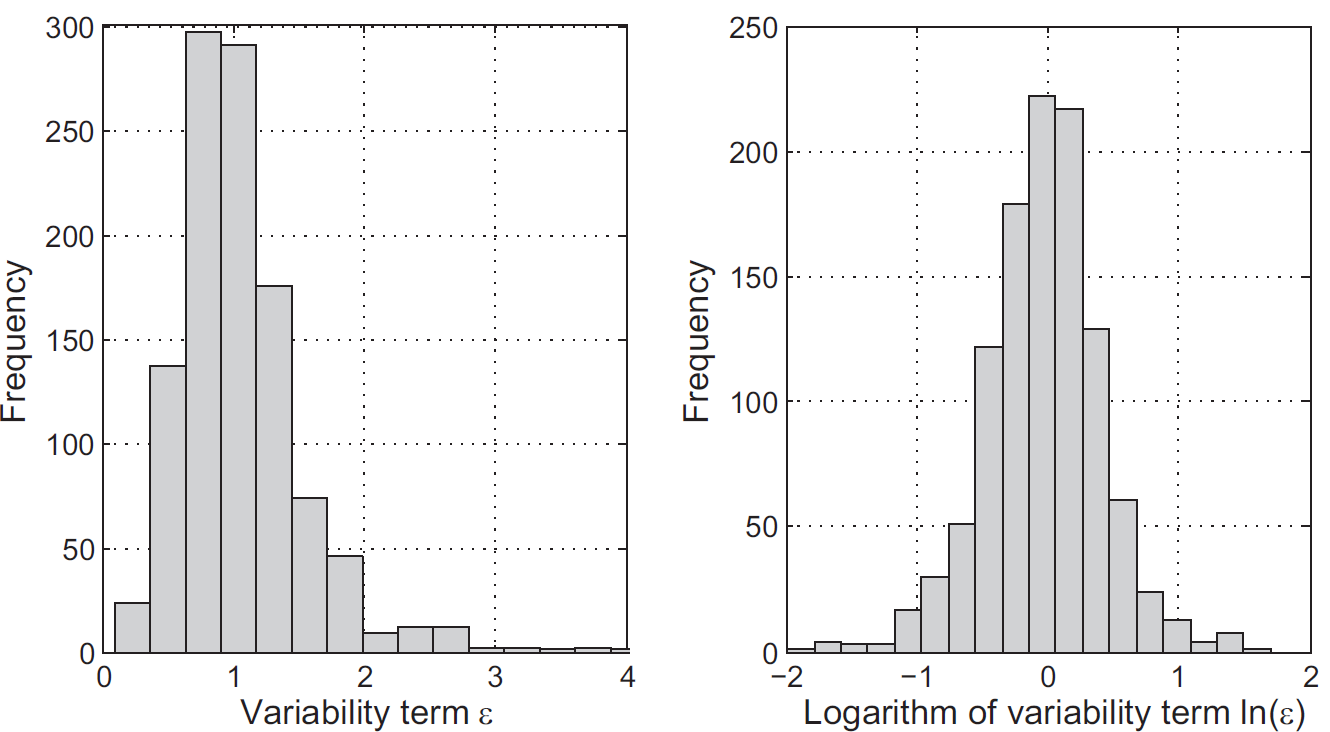
\includegraphics[width=0.5\textwidth]{figures/figure-17.png}
    \caption{Histograms of $\varepsilon$ and $\ln(\varepsilon)$ for the $\rm{OCR}-(s_u/\sigma_v')$ model proposed by \citet{Jamiolkowski198557}.}
    \addtocounter{figure}{-1}
    \vspace{-5pt}
    \renewcommand{\figurename}{图}
    \caption{\citet{Jamiolkowski198557}提出的$\rm{OCR}-(s_u/\sigma_v')$模型的$\varepsilon$和$\ln(\varepsilon)$直方图。}
    \renewcommand{\figurename}{Figure}
    \label{figure:17}
\end{figure*}
    \begin{align}
        \begin{split}
            \rm{Actual~value}&=\rm{predicted~value}\times{}b\times{}\left[\alpha\times{}(\rm{PI}/20)^\beta\right]\times{}\varepsilon'\\
            &=\rm{predicted~value}\times{}b'\times{}\varepsilon'
        \end{split}
        \label{equation:6}
    \end{align}
    \ParallelLText
    {
        where $b'$ is the updated bias factor and can be expressed as the product of the original bias $b$ and a correction term $\alpha\times{}(\rm{PI}/20)^\beta$
    }
    \ParallelRText
    {
        其中$b'$是更新的偏差因子,可以表示为原始偏差$b$与校正项$\alpha\times{}(\rm{PI}/20)^\beta$的乘积
    }
    \ParallelPar
    \begin{align}
        b'=b\times{}\left[\alpha\times{}(\rm{PI}/20)^\beta\right]=b\times{}(\rm{bias~correction~factor})
        \label{equation:7}
    \end{align}
    \ParallelLText
    {
        The term  $\alpha\times{}(\rm{PI}/20)^\beta$ is called the bias correction factor (BCF). In Table \ref{table:6}, the updated bias factors $b'$ are shown in the format of $b'=(\rm{original}~b)\times{}[BCF]$. The sample COV of epsilou (the updated variability term) is denoted by delta. In Table \ref{table:6}, $\delta'$ values are shown in the format of are shown in the format of $\delta'=(\rm{original}~\delta)\times{}(\rm{CCF}\%)$, where CCF denotes the COV correction factor.
    }
    \ParallelRText
    {
        项$\alpha\times{}(\rm{PI}/20)^\beta$称为偏差校正因子(BCF)。在表\ref{table:6}中,更新的偏差因子$b'$以$b'=(\rm{original}~b)\times{}[BCF]$的格式显示。 $\varepsilon'$的样本COV(更新的可变性项)$\delta'$。 在表\ref{table:6}中,$\delta'$以$\delta'=(\rm{original}~\delta)\times{}(\rm{CCF}\%)$的格式显示,其中CCF表示COV校正因子。
    }
    \ParallelPar
    \ParallelLText
    {
        It is apparent that when the target parameter is $\sigma_p'/P_a$ or OCR, the BCFs are always decreasing functions of PI ($\beta<0$). This implies that clays with larger PI values tend to have lower $\sigma_p'/P_a$ and OCR values. For the $\rm{CPTU}-(s_u/\sigma_v')$ model proposed by \citet{Ching201252}, the target parameter is the CPTU cone factors (namely $(q_t-\sigma_v)/s_u$, $(q_t-u_2)/s_u$ and $(u_2-u_0)/s_u$), the BCFs are increasing functions of PI ($\beta>0$). This implies that clays with larger PI tend to have larger cone factors, hence smaller $s_u$. This observation is known (\citealt{Aas19861,Marsland1988209,Powell1988903}) although it has not been established with statistical rigor using such a large database. The CCFs are fairly close to 100$\%$, indicating that the inference using PI does not significantly reduce the transformation uncertainties.
    }
    \ParallelRText
    {
        显然,当目标参数为$\sigma_p'/P_a$或OCR时,BCF始终是PI的递减函数($\beta<0$)。这意味着具有较大PI值的黏土往往具有较低的$\sigma_p'/P_a$和OCR值。 对于\citet{Ching201252}提出的$\rm{CPTU}-(s_u/\sigma_v')$模型,目标参数是CPTU锥因子(即$(q_t-\sigma_v)/s_u$,$(q_t-u_2)/s_u$,以及$(u_2-u_0)/s_u$),BCF是PI的增函数($\beta>0$)。 这意味着具有较大PI的黏土往往具有较大的圆锥系数,因此$s_u$较小。 这种结论是可信的(\citealt{Aas19861,Marsland1988209,Powell1988903}),尽管还没有使用如此庞大的数据库以统计上的严格性来建立它。 CCF相当接近100$\%$,这表明使用PI进行推理并不能显着减少变换的不确定性。
    }
    \ParallelPar
    \ParallelLText
    {
        For the inference using PI and $S_t$, it is possible to express $\varepsilon$ as
    }
    \ParallelRText
    {
        对于使用PI和$S_t$进行推理,可以将$\varepsilon$表示为
    }
    \ParallelPar
    \begin{align}
        \varepsilon=\left[\alpha\times{}(\rm{PI}/20)^\beta\times{}S_t^\gamma\right]\times{}\varepsilon'
        \label{equation:8}
    \end{align}
    \ParallelLText
    {
        The coefficients  $\alpha$,$\beta$ and $\gamma$ can be estimated using linear regression on the $\ln(\varepsilon)-\ln(\rm{PI})-\ln(S_t)$ data points. Namely, the following regression model is used:
    }
    \ParallelRText
    {
        可以使用$\ln(\varepsilon)-\ln(\rm{PI})-\ln(S_t)$数据点上的线性回归来估计系数$\alpha$,$\beta$和$\gamma$。 即使用以下回归模型:
    }
    \ParallelPar
    \begin{align}
        \ln(\varepsilon)\approx{}\ln(\alpha)+\beta\ln(\rm{PI}/20)+\gamma\ln(S_t)
        \label{equation:9}
    \end{align}
    \ParallelLText
    {
        where $\ln(\varepsilon)$ is the known output, and $\ln(\rm{PI}/20)$ and $\ln(S_t)$ are the known inputs, whereas $\ln(\alpha)$, $\beta$ and $\gamma$ are the intersect and gradients to be estimated by the least-squares method. Once the least-squares estimates for $\ln(\alpha)$, $\beta$ and $\gamma$ are obtained, the term $\alpha\times{}(\rm{PI}/20)^\beta\times{}S_y^\gamma$ is now the BCF. Table \ref{table:6} shows the updated bias factors $b'$ in the format of $b'=(\rm{original}~b)\times{}[BCF]$ and the updated $\delta'$ in the format of $\delta'=(\rm{original}~\delta)\times{}(\rm{CCF}\%)$ for the inference using PI and $S_t$. It is apparent that when the target parameter is $s_u/\sigma_v'$ or $s_u/\sigma_p'$, these BCFs are always increasing functions of $S_t$ ($\gamma>0$), implying that clays with larger $S_t$ values tend to have larger $s_u/\sigma_v'$ and $s_u/\sigma_p'$ values. When the target parameter is CPTU cone factors, these BCFs are decreasing functions of $S_t$ ($\gamma<0$). This implies that clays with larger $S_t$ values tend to have smaller cone factors, hence larger $s_u$ values. The updated COV ($\delta'$) is typically noticeably less than the original $\delta$ value in Table \ref{table:5}. There are two possible explanations for such uncertainty reduction:
    }
    \ParallelRText
    {
        其中$\ln(\varepsilon)$是已知输出,而$\ln(\rm{PI}/20)$和$\ln(S_t)$是已知输入,而$\ln(\alpha)$,$\beta$和$\gamma$是通过最小二乘法估计的相交和渐变。一旦获得了$\ln(\alpha)$,$\beta$和$\gamma$的最小二乘估计,则$\alpha\times{}(\rm{PI}/20)^\beta\times{}S_y^\gamma$项即为BCF。表\ref{table:6}显示了使用PI和$S_t$进行推导的的$b'=(\rm{original}~b)\times{}[BCF]$格式的更新的偏差因子$b'$和$\delta'=(\rm{original}~\delta)\times{}(\rm{CCF}\%)$格式的更新的$\delta'$。很明显,当目标参数为$s_u/\sigma_v'$或$s_u/\sigma_p'$,BCF始终是$S_t$的增函数($\gamma>0$),这意味着具有较大$S_t$值的黏土往往具有较大的$s_u/\sigma_v'$和$s_u/\sigma_p'$。当目标参数是CPTU锥因子时,BCF是$S_t$的递减函数($\gamma<0$)。这意味着具有较大$S_t$值的黏土往往具有较小的圆锥系数,因此具有较大的$S_u$值。通常,更新后的COV($\delta'$)明显小于表\ref{table:5}中的原始$\delta$值。对于这种降低不确定性有两种可能的解释:
    }
    \ParallelPar
    \ParallelLText
    {
        1. The uncertainty is indeed effectively reduced with the inclusion of $S_t$ as a secondary explanatory variable.

        2. The number of $\ln(\varepsilon)-\ln(\rm{PI})-\ln(S_t)$ data points is substantially less than the number of $\ln(\varepsilon)-\ln(\rm{PI})$ data points (see the “$n$” column in Table \ref{table:5}). The former $n$ is typically around 100 to 200, except two models where $n$ is around 400, while the latter $n$ is about 2 to 5 times more. These relatively small numbers of the $\ln(\varepsilon)-\ln(S_t)$ data points may not represent a “global” dataset. Hence, the resulting $\delta'$ may look small.
    }
    \ParallelRText
    {
        1.通过将$S_t$作为次要解释变量,确实可以有效降低不确定性。

        2. $\ln(\varepsilon)-\ln(\rm{PI})-\ln(S_t)$数据点的数量大大少于$\ln(\varepsilon)-\ln(\rm{PI})$数据点的数量(请参见表\ref{table:5}中的“$n$”列)。前者的$n$通常约为100到200,只有两个模型的$n$约为400,而后者的$n$大约是后者的2至5倍。 这些相对较少的$\ln(\varepsilon)-\ln(S_t)$数据点可能无法表示“全局”数据集。 因此,所得的$\delta'$看起来可能很小。
    }
\end{Parallel}

\section{Implementation 实现}

\begin{paracol}{2}
    
    \autoref{table:5} and \autoref{table:6} are useful for obtaining first-order estimates of the mean and COV of a clay parameter of interest (e.g., $s_u$ or $\sigma_p'$) based on the test index at hand. These mean and COV estimates are essential for RBD. First of all, it is imperative to determine whether a transformation model is consistent with the CLAY/10/7490 database by checking the column “Comparison to the global database” and subcolumn “Fit to the trend?”. It is recommended to only adopt models that fit to the CLAY/10/7490 database. Using the well-known model developed by \citet{Jamiolkowski198557} as an example, suppose OCR = 2 is known, and the goal is to determine the mean and COV of $s_u(\rm{mob})/\sigma_v'$. According to \autoref{table:5}, this model fits well to the CLAY/10/7490 database and this fit is shown in \autoref{figure:10}. The second step is to extract the bias factor $b = 1.11$ and COV = 0.53 from the column “Calibration results”. Then, the mean of $s_u(\rm{mob})/\sigma_v'$ is computed as $b\times{}0.23\times{}\rm{OCR}^{0.8}=1.11\times{}0.23\times{}2^{0.8}=0.44$ and the data scatter around the mean is quantified by COV = 0.53.
        
    \switchcolumn
    
    \cntableref{table:5}和\cntableref{table:6}用于基于手边的测试指数获得感兴趣的黏土参数(例如,$s_u$或$\sigma_p'$)的平均值和COV的一阶估计。这些均值和COV估计值对于RBD至关重要。首先,必须通过检查“与全局数据库比较”列和“适应趋势?”列来确定转换模型是否与CLAY/10/7490数据库一致。建议仅采用适合CLAY/10/7490数据库的模型。使用\citet{Jamiolkowski198557}开发的著名模型作为一个例子,假设OCR = 2是已知的,目标是确定$s_u(\rm{mob})/\sigma_v'$的平均值和COV。根据\cntableref{table:5},此模型非常适合CLAY/10/7490数据库,并且该适合关系如\cnfigureref{figure:10}所示。第二步是从“校准结果”列中提取偏差因子$b = 1.11$和COV = 0.53。然后,将$s_u(\rm{mob})/\sigma_v'$的平均值计算为$b\times{}0.23\times{}\rm{OCR}^{0.8}=1.11\times{}0.23\times{}2^{0.8}=0.44$,并用COV = 0.53量化围绕平均值的数据散布。
        
    \switchcolumn*
    
    In the case where PI = 15 and $S_t$ = 10 information is also available, one can extract the bias correction factor (BCF) and COV correction factor (CCF) from the column “Inference results” and subcolumn “Inference based on PI and $S_t$” in \autoref{table:6}. Thus, BCF = $0.71\times{}(PI/20)^{0.133}\times{}S_t^{0.123} = 0.71\times{}(15/20)^{0.133}\times{}10^{0.123} = 0.907$ and CCF = 67$\%$. As a result, the mean for $s_u(\rm{mob})/\sigma_v'$ becomes $0.44\times{}0.907 = 0.403$ and the COV becomes $0.53\times{}67\%= 0.36$. Updating the mean and COV of $s_u(\rm{mob})/\sigma_v'$ based on other measured pieces of information (for example, PI, $S_t$, $(q_t-\sigma_v)/\sigma_v'$, and $B_q$ may have been simultaneously measured in close proximity at the same depth in a site investigation report) is possible once the multivariate probability distribution among these clay parameters is established. This is addressed in a companion paper \citep{Ching2014686}.
        
    \switchcolumn
    
    如果还提供PI = 15和$S_t$ = 10的信息,则可以从“推断结果”列和子列“基于PI和$S_t$的推断”中提取偏差校正因子(BCF)和COV校正因子(CCF)。 因此,\cntableref{table:6}中的BCF=$0.71\times{}(PI/20)^{0.133}\times{}S_t^{0.123} = 0.71\times{}(15/20)^{0.133}\times{}10^{0.123} = 0.907$,CCF = 67$\%$。 结果,$s_u(\rm{mob})/\sigma_v'$的平均值为$0.44\times{}0.907 = 0.403$,COV为$0.53\times{}67\%= 0.36$。 根据其他测得的信息(例如,PI,$S_t$,$(q_t-\sigma_v)/\sigma_v'$和$B_q$可能同时在附近测量)更新$s_u(\rm{mob})/\sigma_v'$的平均值和COV。 一旦在这些黏土参数之间建立了多元概率分布,就可能实现相同的深度。 伴随文件对此进行了阐述\citep{Ching2014686}。
        
\end{paracol}

\section{Conclusions 结论}

\begin{paracol}{2}

    In this paper, a global clay database is presented, and 24 transformation models among clay parameters in the literature are investigated. This database contains clays with a wide range of $S_t$, OCR, and PI values and from a wide range of geographical locales. It is found that most of the 24 models fit to the data trends of the global database. There are few exceptions, and it is believed that the poor fit is due to the fact that these models were developed by databases with a limited range of clay types (e.g., no quick clays are in the database or only clays of a single region were in the database).
        
    \switchcolumn
    
    本文提出了一个全球黏土数据库,并研究了文献中24个黏土参数之间的转换模型。 该数据库包含具有广泛的$S_t$,OCR和PI值且来自不同地理位置的粘土。 发现这24个模型中的大多数都适合于全球数据库的数据趋势。 几乎没有例外,并且认为拟合度较差是由于以下事实:这些模型是由黏土类型范围有限的数据库开发的(例如,数据库中没有快速黏土,或者只有单个区域的黏土在数据库中)。
        
    \switchcolumn*
    
    The global database is further used to calibrate the biases and uncertainties for the models in literature. It is found that more recent models tend to have smaller biases. Also, the uncertainties calibrated by the global database are mostly larger than the uncertainties reported in the literature. The large uncertainties may be reduced by considering PI and $S_t$ as secondary input parameters for the models. The biases are also updated after incorporating PI and $S_t$.
        
    \switchcolumn
    
    全球数据库还用于校准文献中模型的偏差和不确定性。 已经发现,较新的模型倾向于具有较小的偏差。 此外,由全球数据库校准的不确定性大多大于文献中报道的不确定性。 通过将PI和$S_t$作为模型的辅助输入参数,可以减少较大的不确定性。 在合并PI和$S_t$之后,偏差也会更新。
        
\end{paracol}

\begin{appendix}
    \section{Summary of database CLAY/10/7490 数据库CLAY/10/7490概览}\label{appendix:a}
    \small
\setlength{\tabcolsep}{0.5mm}{\begin{longtable}{lllllllll}
    \caption{Basic information of the database CLAY/10/7490.\\表7:数据库CLAY/10/7490的详细信息}\label{table:7}\\
    \toprule
    Reference & Country & $n$ & PI & LI & OCR & $S_t$ & $s_u(\rm{mob})/\sigma_v'$ & CPTU \\
    \midrule
    \endfirsthead
    \multicolumn{9}{l}{(Continued to Table \ref{table:7})} \\
    \toprule
    Reference & Country & $n$ & PI & LI & OCR & $S_t$ & $s_u(\rm{mob})/\sigma_v'$ & CPTU \\
    \midrule
    \endhead
    \bottomrule
    \multicolumn{9}{l}{(Continued on next page)}
    \endfoot
    \bottomrule
    \endlastfoot
    \citet{Aas19861} & Norway & 12    & $-$     & $-$     & 1.5$\sim$10.0 & $-$     & $-$     & $-$ \\
    \citet{Aas198021} & Norway & 2     & $-$     & $-$     & $-$     & $-$     & 0.30$\sim$0.33 & $-$ \\
    \citet{Agarwal1967} & UK    & 22    & $-$     & $-$     & $-$     & $-$     & 0.09$\sim$0.61 & $-$ \\
    \citet{Akai1965146} & Japan & 6     & 27    & 0.54  & $-$     & $-$     & $-$     & $-$ \\
    \citet{Alberro19731} & Mexico & 85    & 284$\sim$363 & 0.71$\sim$1.19 & $-$     & $-$     & 0.03$\sim$0.68 & $-$ \\
    \citet{Amerasinghe19751277} & UK    & 28    & $-$     & $-$     & $-$     & $-$     & 0.29$\sim$4.57 & $-$ \\
    \citet{Andersen1982918} & Brazil & 16    & 47$\sim$102 & 1.09$\sim$1.63 & 1.6$\sim$7.4 & 2$\sim$5   & 0.31$\sim$5.44 & $-$ \\
    \citet{Andersen1980499} & Norway & 11    & $-$     & $-$     & 1.0$\sim$50.0 & $-$     & 0.04$\sim$7.78 & $-$ \\
    \citet{Andresen195754} & Norway & 18    & 12$\sim$32 & 0.48$\sim$0.95 & $-$     & 2$\sim$5   & $-$     & $-$ \\
    \citet{Andersen1982918} & Norway & 3     & $-$     & $-$     & 1.6$\sim$40.0 & $-$     & $-$     & $-$ \\
    \citet{Azzouz1986389} & USA   & 33    & 29$\sim$69 & 0.18$\sim$0.47 & 1.0$\sim$1.4 & $-$     & 0.04$\sim$0.20 & Y \\
    \citet{Azzouz1983161} & Venezuela & 10    & 42$\sim$57 & 0.45$\sim$0.78 & 1.1$\sim$3.3 & $-$     & 0.14$\sim$0.20 & Y \\
    \citet{Balasubramaniam1976390} & Thailand & 10    & 82    & $-$     & $-$     & $-$     & 0.07$\sim$0.87 & $-$ \\
    \citet{Baligh1980447} & USA   & 20    & 13$\sim$72 & 0.23$\sim$1.48 & 1.1$\sim$5.4 & $-$     & 0.22$\sim$1.40 & Y \\
    \citet{Banerjee197835} & UK    & 2     & 26    & 0.36$\sim$0.38 & 1.0$\sim$1.2 & $-$     & 0.15$\sim$0.22 & $-$ \\
    \citet{Baracos1980559} & Canada & 9     & 36$\sim$64 & -0.01$\sim$0.60 & 2.8$\sim$9.2 & $-$     & 0.09$\sim$4.43 & $-$ \\
    \citet{Battaglio1986129} & Italy & 15    & $-$     & $-$     & 21.0$\sim$36.4 & $-$     & $-$     & Y \\
    \citet{Berre197339} & Norway & 14    & 10$\sim$88 & 0.61$\sim$1.04 & 1.0$\sim$1.8 & 5$\sim$11  & 0.19$\sim$0.41 & $-$ \\
    \citet{Bishop19713} & UK    & 14    & 39    & 0.06$\sim$0.21 & 2.1$\sim$16.0 & 1$\sim$2   & 0.39$\sim$4.89 & $-$ \\
    \citet{Bishop19651} & UK    & 6     & 36$\sim$43 & -0.14$\sim$-0.04 & $-$     & $-$     & $-$     & $-$ \\
    \citet{Bjerrum195449} & Norway & 246   & 3$\sim$33  & -0.05$\sim$4.70 & $-$     & 3$\sim$500 & 5.4   & $-$ \\
    \citet{Bjerrum1960711} & $-$     & 35    & 7$\sim$92  & 0.28$\sim$3.43 & $-$     & 2$\sim$100 & $-$     & $-$ \\
    \citet{Bjerrum1963147} & Norway & 68    & 22$\sim$32 & 0.60$\sim$0.81 & $-$     & 5     & 0.22$\sim$45.02 & $-$ \\
    \citet{Bjerrum196783} & Norway & 89    & 4$\sim$41  & 0.61$\sim$3.22 & $-$     & 2$\sim$300 & 0.05$\sim$0.25 & $-$ \\
    \citet{Bjerrum1969377} & Norway & 14    & 13$\sim$27 & 1.46$\sim$2.12 & $-$     & $-$     & $-$     & $-$ \\
    \citet{Bjerrum19721} & $-$     & 6     & 11$\sim$85 & 0.3$\sim$1.1 & $-$     & $-$     & $-$     & $-$ \\
    \citet{Bjerrum1973111} & Norway & 6     & 3$\sim$31  & 0.75$\sim$5.3 & $-$     & 8$\sim$100 & 0.16$\sim$0.30 & $-$ \\
    \citet{Bozozuk1972299} & Canada & 19    & 20$\sim$34 & 1.18$\sim$2.49 & 1.3$\sim$2.0 & 8$\sim$100 & 0.13$\sim$0.55 & $-$ \\
    \citet{Broms19631} & Norway & 3     & $-$     & $-$     & 3.5$\sim$13.0 & $-$     & $-$     & $-$ \\
    \citet{Burland1977557} & UK    & 14    & 19$\sim$46 & -0.19$\sim$-0.01 & $-$     & $-$     & 0.59$\sim$2.43 & $-$ \\
    \citet{Cadling19501} & Sweden & 136   & 22$\sim$88 & 0.77$\sim$1.24 & $-$     & 2$\sim$167 & 0.06$\sim$0.29 & $-$ \\
    \citet{Calabresi1973233} & Italy & 1     & 33    & 0.24  & $-$     & $-$     & $-$     & $-$ \\
    \citet{Campanella1988203} & Canada & 20    & $-$     & $-$     & 1.0$\sim$4.5 & 12$\sim$25 &       & Y \\
    \citet{Cancelli1981377} & Italy & 13    & 20$\sim$39 & 0.03$\sim$0.26 & $-$     & $-$     & 0.14$\sim$1.79 & $-$ \\
    \citet{Cancelli1984637} & Italy & 5     & 31$\sim$39 & 0.04$\sim$0.44 & 1.0$\sim$26.7 & $-$     & 0.23$\sim$4.00 & Y \\
    \citet{Carrier1984211} & USA   & 14    & 110$\sim$165 & 0.5$\sim$1.43 & $-$     & $-$     & $-$     & $-$ \\
    \citet{Carter1991} & UK    & 24    & $-$     & -0.11$\sim$1.90 & $-$     & 1$\sim$141 & $-$     & $-$ \\
    \citet{Chandler1969321} & UK    & 1     & 10    & -0.75 & $-$     & $-$     & $-$     & $-$ \\
    \citet{Chandler198813} & $-$     & 22    & 4$\sim$100 & 0.47$\sim$4 & 1$\sim$6.3 & 2$\sim$80  & 0.15$\sim$0.36 & $-$ \\
    \citet{Chang1991210} & Singapore & 13    & 18$\sim$87 & 0.33$\sim$0.95 & 0.8$\sim$1.9 & 3.1   & 0.10$\sim$0.62 & Y \\
                         & Malaysia & 11    & 33$\sim$79 & 0.51$\sim$1.77 & 1.3$\sim$3.5 & 3.6$\sim$5.0 & 0.26$\sim$0.63 & Y \\
    \citet{Chen199655} & Taiwan & 23    & 11$\sim$24 & 0.64$\sim$1.36 & 1.1$\sim$1.5 & 4$\sim$5   & $-$     & Y \\
    \citet{Chen200129} & Taiwan & 12    & $-$     & $-$     & $-$     & $-$     & $-$     & $-$ \\
    \citet{Chen19931732} & $-$     & 195   & 9$\sim$85  & -0.44$\sim$2.40 & 1.0$\sim$39.0 & 3$\sim$128 & 0.03$\sim$2.48 & $-$ \\
    \citet{Chin1997665} & Taiwan & 12    & $-$     & $-$     & 1.0$\sim$4.1 & $-$     & 0.18$\sim$0.90 & $-$ \\
    \citet{Chin1989245} & Taiwan & 32    & 8$\sim$26  & $-$     & 1.0$\sim$8.0 & $-$     & $-$     & $-$ \\
    \citet{Clough198045} & China & 29    & 35$\sim$52 & 0.51$\sim$1.95 & $-$     & $-$     & 0.09$\sim$0.23 & $-$ \\
    \citet{Cooling1942251} & UK    & 113   & 36$\sim$67 & -0.03$\sim$0.06 & $-$     & $-$     & $-$     & $-$ \\
    \citet{Coutinho20072049} & Brazil & 12    & 27$\sim$168 & 0.50$\sim$2.23 & 0.9$\sim$2.2 & 5$\sim$14  & 0.24$\sim$0.91 & Y \\
    \citet{Cox19791147} & USA   & 51    & 10$\sim$69 & 0.05$\sim$0.80 & $-$     & $-$     & $-$     & $-$ \\
    \citet{Crawford195936} & Canada & 3     & 14$\sim$27 & 0.53$\sim$1.21 & $-$     & 3$\sim$6   & $-$     & $-$ \\
    \citet{Crawford1964227} & Canada & 9     & $-$     & $-$     & $-$     & $-$     & $-$     & $-$ \\
    \citet{Crawford1991103} & Canada & 8     & $-$     & $-$     & 1.4$\sim$3.8 & 20$\sim$122 & $-$     & Y \\
    \citet{Crawford196531} & Canada & 10    & 14$\sim$36 & 0.9$\sim$2.5 & 1.5$\sim$7.9 & 10$\sim$500 & 0.31$\sim$2.63 & $-$ \\
    \citet{Croce196981} & Italy & 14    & 23$\sim$47 & -0.11$\sim$0.55 & 1.5$\sim$4.7 & 1$\sim$8   & 0.07$\sim$1.30 & $-$ \\
    \citet{Crooks1981685} & Northern Ireland & 15    & $-$     & $-$     & 1.4$\sim$2.8 & $-$     & 0.31$\sim$0.71 & $-$ \\
    \citet{Crooks1976293} & Canada & 22    & 22$\sim$63 & 0.61$\sim$1.37 & 0.9$\sim$1.7 & 4$\sim$10  & $-$     & $-$ \\
    \citet{Cummings1950275} & USA   & 10    & 4$\sim$18  & 0.20$\sim$0.97 & $-$     & $-$     & $-$     & $-$ \\
    \citet{D'Appolonia1971881} & USA   & 1     & 17    & 0.7   & 9.3   & $-$     & 0.77  & $-$ \\
    \citet{D'Appolonia1972126} & Norway & 104   & $-$     & $-$     & 1.0$\sim$37.5 & $-$     & $-$     & $-$ \\
    \citet{DaCruz196373} & Brazil & 15    & $-$     & $-$     & 0.6$\sim$3.4 & $-$     & $-$     & $-$ \\
    \citet{Dascal1975297} & Canada & 11    & 9$\sim$12  & 1.11$\sim$3.89 & 1.4$\sim$35.8 & $-$     & 0.28$\sim$0.85 & $-$ \\
    \citet{DeGroot2003695} & USA   & 64    & 11$\sim$30 & 0.04$\sim$2.87 & 1.4$\sim$9.5 & 6$\sim$43  & 0.17$\sim$1.25 & $-$ \\
    \citet{DeLory19671} & Canada & 40    & 19$\sim$59 & 0.84$\sim$1.31 & $-$     & $-$     & 0.13$\sim$1.84 & $-$ \\
    \citet{DeLory196997} & Canada & 33    & 17$\sim$46 & 0.50$\sim$1.94 & $-$     & $-$     & 0.13$\sim$0.32 & $-$ \\
    \citet{DiBiagio19769} & Norway & 6     & 5$\sim$11  & 1.68$\sim$3.71 & $-$     & 18$\sim$74 & $-$     & $-$ \\
    \citet{Donaghe1978173} & USA   & 28    & $-$     & $-$     & $-$     & $-$     & 0.02$\sim$1.05 & $-$ \\
    \citet{Duncan196621} & USA   & 10    & $-$     & $-$     & 3.0$\sim$18.0 & $-$     & 0.33$\sim$1.35 & $-$ \\
    \citet{Eden196254} & Canada & 9     & 15$\sim$40 & 1.32$\sim$2.12 & 1.2$\sim$1.9 & 8$\sim$18  & 0.31$\sim$0.38 & $-$ \\
    \citet{Eden195722} & Canada & 36    & 5$\sim$56  & 0.81$\sim$4.13 & 1.6$\sim$4.4 & 36$\sim$1467 & 0.49$\sim$1.46 & $-$ \\
    \citet{Eden195741} & Canada & 49    & 5$\sim$56  & 0.63$\sim$4.4 & 1.0$\sim$3.5 & 4$\sim$1160 & 0.26$\sim$2.64 & $-$ \\
    \citet{Eden19611239} & Canada & 113   & $-$     & 0.66$\sim$3.10 & $-$     & 1$\sim$307 & $-$     & $-$ \\
    \citet{Eden1980369} & Canada & 5     & 28$\sim$46 & $-$     & 2.0$\sim$3.0 & $-$     & 0.53$\sim$1.03 & Y \\
    \citet{Eden196828} & Canada & 12    & 18$\sim$26 & 0.57$\sim$2.90 & $-$     & $-$     & $-$     & $-$ \\
    \citet{Egashira1982275} & Japan & 14    & 8$\sim$96  & 0.48$\sim$3.63 & $-$     & 19$\sim$970 & $-$     & $-$ \\
    \citet{Eide1972159} & Thailand & 9     & 83$\sim$108 & 0.76$\sim$0.93 & 1.6$\sim$2.2 & 6$\sim$10  & 0.33$\sim$0.47 & $-$ \\
    \citet{Endley1979101} & USA   & 24    & 13$\sim$56 & -0.10$\sim$0.69 & $-$     & $-$     & $-$     & $-$ \\
    \citet{Esu1969555} & Italy & 3     & 44$\sim$51 & 0.1$\sim$0.16 & $-$     & $-$     & $-$     & $-$ \\
    \citet{Feyling-Hanssen1957} & Norway & 10    & 8$\sim$26  & -0.20$\sim$0.88 & $-$     & $-$     & $-$     & $-$ \\
    \citet{Finno19891} & USA   & 17    & 15$\sim$21 & 0.20$\sim$2.59 & 0.8$\sim$4.2 & 2$\sim$3   & $-$     & Y \\
    \citet{Flaate197472} & Norway & 18    & 6$\sim$33  & 0.09$\sim$0.48 & $-$     & $-$     & 0.06$\sim$0.91 & $-$ \\
    \citet{Focht199176} & Mexico & 108   & 8$\sim$41  & -0.52$\sim$3.95 & $-$     & $-$     & 0.07$\sim$27.75 & $-$ \\
    \citet{Gregersen1979535} & Norway & 19    & 6$\sim$13  & 0.56$\sim$2.67 & $-$     & 13    & $-$     & $-$ \\
    \citet{Gregersen1979183} & Norway & 37    &       & 0.14$\sim$2.46 & $-$     & 2$\sim$185 & $-$     & $-$ \\
    \citet{Hansen1980253} & $-$     & 8     & 10$\sim$105 & 0.65$\sim$1.04 & $-$     & 5$\sim$11  & $-$     & $-$ \\
    \citet{Hanzawa197717} & Iraq  & 11    & 34$\sim$36 & 0.62$\sim$0.73 & $-$     & $-$     & 0.83$\sim$2.35 & $-$ \\
    \citet{Hanzawa19771} & Iraq  & 31    & 11$\sim$31 & 0.65$\sim$1.10 & 1     & $-$     & 0.09$\sim$0.37 & $-$ \\
    \citet{Hanzawa197969} & Japan & 60    & $-$     & $-$     & $-$     & $-$     & $-$     & $-$ \\
    \citet{Hanzawa19791} & Iraq  & 12    & 35$\sim$38 & 0.63$\sim$0.66 & 1.3$\sim$5.7 & $-$     & 0.32$\sim$0.92 & $-$ \\
    \citet{Hanzawa1981683} & Japan & 3     & $-$     & $-$     & $-$     & $-$     & 0.20$\sim$0.23 & $-$ \\
    \citet{Hara19741} & Japan & 182   & 10$\sim$92 & $-$     & 1.0$\sim$3.0 & $-$     & $-$     & $-$ \\
    \citet{Harris1995293} & France & 67    & $-$     & 0.33$\sim$1.66 & $-$     & $-$     & $-$     & $-$ \\
    \citet{Helenelund1977} & Sweden & 36    & 22$\sim$94 & $-$     & $-$     & $-$     & 0.15$\sim$0.31 & $-$ \\
    \citet{Henkel1963280} & England & 59    & $-$     & $-$     & $-$     & $-$     & $-$     & $-$ \\
    \citet{Henry1957275} & Hong Kong & 22    & $-$     & $-$     & $-$     & $-$     & $-$     & $-$ \\
    \citet{Hight1992303} & UK    & 9     & 24$\sim$44 & $-$     & 1.3$\sim$1.6 & $-$     & 0.38$\sim$0.64 & Y \\
    \citet{Holmberg19771} & Thailand & 52    & 57$\sim$105 & 0.63$\sim$1.16 & 1.4$\sim$2.5 & 5$\sim$15  & 0.20$\sim$4.72 & $-$ \\
    \citet{Holtz19721223} & USA   & 22    & 10$\sim$16 & -0.45$\sim$0.45 & $-$     & $-$     & $-$     & $-$ \\
    \citet{Holtz197979} & Sweden & 13    & 74$\sim$114 & 0.66$\sim$0.99 & 1.3$\sim$3.0 & $-$     & $-$     & $-$ \\
    \citet{Hong20102} & Korea & 17    & $-$     & $-$     & $-$     & $-$     & 0.17$\sim$0.27 & Y \\
    \citet{Horn1964215} & USA   & 12    & 14$\sim$31 & 0.37$\sim$0.81 & 0.8$\sim$4.0 & 4$\sim$10  & 0.07$\sim$0.50 & $-$ \\
    \citet{Hutchinson19696} & UK    & 2     & 31$\sim$51 & -0.16$\sim$0.02 & $-$     & $-$     & $-$     & $-$ \\
    \citet{Jamiolkowski1988263} & Italy & 17    & $-$     & $-$     & 7.9$\sim$20.7 & $-$     & $-$     & $-$ \\
    \citet{Janbu197795} & Norway & 7     & 3$\sim$11  & -0.25$\sim$0.71 & $-$     & 3$\sim$14  & $-$     & $-$ \\
    \citet{Jardine2003599} & UK    & 13    & 41$\sim$95 & 0.44$\sim$0.98 & $-$     & 1$\sim$11  & $-$     & $-$ \\
    \citet{Karlsrud1976157} & Norway & 25    & 20$\sim$27 & 0.60$\sim$3.60 & $-$     & $-$     & 0.17$\sim$0.64 & $-$ \\
    \citet{Karlsson196735} & Sweden & 11    & 24$\sim$42 & 0.34$\sim$2.75 & $-$     & 14$\sim$307 & 0.23$\sim$1.37 & $-$ \\
    \citet{Kenney1966} & Norway & 40    & 10$\sim$36 & 0.52$\sim$2.86 & $-$     & 3$\sim$60  & 0.02$\sim$2.71 & $-$ \\
    \citet{Kinner1970} & USA   & 62    & $-$     & $-$     & 1.0$\sim$24 & $-$     & 0.05$\sim$2.07 & $-$ \\
    \citet{Kitago1976239} & Japan & 4     & $-$     & $-$     & $-$     & $-$     & $-$     & $-$ \\
    \citet{Kjekstad198150} & Norway & 29    & 19$\sim$34 & -0.15$\sim$0.28 & $-$     & $-$     & 0.26$\sim$1.64 & $-$ \\
    \citet{Konrad1987392} & Canada & 29    & 3$\sim$37  & 0.50$\sim$4.51 & 1.0$\sim$4.9 & 7$\sim$35  & 0.34$\sim$1.66 & Y \\
    \citet{Konrad1987177} & Canada & 17    & $-$     & $-$     & 1.0$\sim$2.6 & $-$     &       & Y \\
    \citet{Koumoto199095} & Japan & 58    & 43$\sim$298 & 0.16$\sim$1.24 & $-$     & $-$     & $-$     & $-$ \\
    \citet{Koumoto2001701} & Japan & 74    & 14$\sim$293 & 0.00$\sim$1.45 & $-$     & $-$     & $-$     & $-$ \\
    \citet{Koutsoftas1976989} & USA   & 95    & 13$\sim$50 & 0.28$\sim$1.14 & 1.0$\sim$29.5 & 108$\sim$414 & 0.19$\sim$2.55 & $-$ \\
    \citet{Koutsoftas1978609} & USA   & 21    & 13$\sim$41 & 0.66$\sim$1.17 & 1.0$\sim$4.0 & $-$     & $-$     & $-$ \\
    \citet{Koutsoftas1981254} & USA   & 19    & $-$     & $-$     & 1.0$\sim$11.7 & $-$     & 0.20$\sim$1.72 & $-$ \\
    \citet{Koutsoftas1985337} & USA   & 20    & $-$     & $-$     & 1.0$\sim$7.7 & $-$     & 0.23$\sim$1.16 & $-$ \\
    \citet{Koutsoftas198787} & Hong Kong & 13    & 12$\sim$66 & 0.19$\sim$1.82 & 1.9$\sim$3.8 & 5.5   & 0.33$\sim$1.13 & Y \\
    \citet{Kulhawy1990} & $-$     & 159   & 9$\sim$80  & -0.44$\sim$2.4 & 1     & $-$     & 0.14$\sim$0.27 & $-$ \\
    \citet{Kulkarani1967210} & India & 5     & 39$\sim$65 & 0.57$\sim$1.00 & 0.7$\sim$1.0 & 3$\sim$4   & 0.12$\sim$0.23 & $-$ \\
    \citet{Lacasse1977367} & Canada & 20    & $-$     & $-$     & 1.0$\sim$2.9 & $-$     & $-$     & $-$ \\
          & USA   & 7     & $-$     & $-$     & 1.0$\sim$4.8 & $-$     & $-$     & $-$ \\
    \citet{Lacasse1981507} & Norway & 11    & $-$     & $-$     & 1.1$\sim$2.7 & $-$     & 0.19$\sim$0.45 & $-$ \\
    \citet{Lacasse1985887} & Norway & 17    & 4$\sim$43  & 0.94$\sim$5.50 & 1.4$\sim$7.1 & $-$     & 0.24$\sim$0.65 & $-$ \\
    \citet{Ladd1964103} & USA   & 22    & $-$     & $-$     & 5.7$\sim$6.2 & $-$     & 0.09$\sim$2.07 & $-$ \\
    \citet{Ladd1965282} & USA   & 8     & $-$     & $-$     & $-$     & $-$     & 0.21$\sim$0.67 & $-$ \\
    \citet{Ladd1967112} & USA   & 16    &       & $-$     & $-$     & $-$     & $-$     & $-$ \\
    \citet{Ladd1972101} & USA   & 43    & 8$\sim$29  & 0.60$\sim$2.52 & 1.3$\sim$7.8 & $-$     & 0.23$\sim$1.84 & $-$ \\
    \citet{Ladd1973108} & USA   & 12    & $-$     & $-$     & $-$     & $-$     & $-$     & $-$ \\
    \citet{Ladd1981643} & USA   & 7     & 20$\sim$55 & $-$     & $-$     & $-$     & 0.11$\sim$0.22 & $-$ \\
    \citet{Ladd1991540} & USA   & 100   & 5$\sim$85  & 1.08$\sim$2.32 & 1.0$\sim$16.4 & 4$\sim$8   & 0.07$\sim$0.81 & $-$ \\
    \citet{Ladd1971}& USA   & 6     & 45    & 1.04  & 1.0$\sim$8.1 & 8     & 0.20$\sim$0.94 & $-$ \\
    \citet{Ladd1972211} & USA   & 14    & 7$\sim$23  & 0.78$\sim$2.52 & 1.3$\sim$2.8 & 7$\sim$10  & 0.20$\sim$1.50 & $-$ \\
    \citet{Ladd1977421} & $-$     & 10    & $-$     & $-$     & 3.0$\sim$18.2 & $-$     & $-$     & $-$ \\
    \citet{Ladd198365} & Venezuela & 75    & 12$\sim$57 & -0.67$\sim$0.67 & 1.0$\sim$2.7 & $-$     & 0.16$\sim$0.57 & $-$ \\
    \citet{Ladd1971} & USA   & 108   & 7$\sim$88  & $-$     & 1.0$\sim$12.1 & 5$\sim$100 & 0$\sim$1.60 & $-$ \\
    \citet{Ladd1974763} & USA   & 22    & 10$\sim$39 & 0.57$\sim$2.68 & 1.0$\sim$4.9 & $-$     & 0.17$\sim$4.37 & $-$ \\
    \citet{Ladd1963342} & $-$     & 39    & 8$\sim$80  & $-$     & 1.0$\sim$3.0 & 5$\sim$10  & 0.07$\sim$0.61 & $-$ \\
    \citet{Lafleur1988705} & Canada & 10    & 33$\sim$47 & 1.21$\sim$1.72 & 1.1$\sim$6.1 & 14    & 0.26$\sim$1.42 & Y \\
    \citet{Lacasse1982661} & Norway & 109   & 16$\sim$72 & 0.28$\sim$1.87 & 1.0$\sim$13.5 & 3$\sim$7   & 0.05$\sim$1.95 & Y \\
    \citet{Lambe196443} & Venezuela & 10    & $-$     & $-$     & $-$     & $-$     & 0.06$\sim$0.24 & $-$ \\
    \citet{LaRochelle1974142} & Canada & 23    & 8$\sim$35  & 1.14$\sim$3.25 & 2.0$\sim$5.2 & $-$     & 0.52$\sim$0.98 & $-$ \\
    \citet{LaRochelle1988831} & Canada & 3     & 15$\sim$44 & 1.39$\sim$1.69 & 1.1$\sim$3.5 & $-$     & 0.24$\sim$0.53 & Y \\
    \citet{Larsson1980591} & Norway & 4     & 7$\sim$53  & $-$     & $-$     & $-$     & 0.19$\sim$0.25 & $-$ \\
    \citet{Larsson1991} & Sweden & 50    & 29$\sim$86 & 0.84$\sim$1.49 & 1.1$\sim$4.2 & $-$     & 0.20$\sim$0.67 & Y \\
    \citet{Landva1988138} & Canada & 26    & 6$\sim$21  & 0.74$\sim$2.63 & 2.2$\sim$4.0 & $-$     & $-$     & $-$ \\
    \citet{Leathers1978250} & USA   & 7     & 32$\sim$46 & 0.66$\sim$1.00 & 1.1$\sim$9.9 & $-$     & 0.28$\sim$0.94 & $-$ \\
    \citet{Lefebvre1987476} & Canada & 26    & $-$     & $-$     & $-$     & $-$     & 0.19$\sim$0.25 & $-$ \\
    \citet{LemboFazio1984115} & Italy & 1     & 28    & -0.25 & $-$     & $-$     & $-$     & $-$ \\
    \citet{Leon1977193} & Mexico & 7     & $-$     & $-$     & $-$     & $-$     & $-$     & $-$ \\
    \citet{Leroueil1983477} & Canada & 10    & 20$\sim$43 & 1.11$\sim$2.87 & 1.4$\sim$2.6 & $-$     & 0.37$\sim$0.76 & $-$ \\
    \citet{Lew1981} & Canada & 6     & $-$     & $-$     & $-$     & $-$     & 0.04$\sim$0.15 & $-$ \\
    \citet{Liu1999} & Taiwan & 53    & 6$\sim$26  & $-$     & $-$     & $-$     & 0.18$\sim$0.37 & $-$ \\
    \citet{Lo19631} & Canada & 13    & 49$\sim$55 & $-$     & $-$     & $-$     & $-$     & $-$ \\
    \citet{Locat1988799} & Canada & 49    & 11$\sim$37 & 0.59$\sim$2.44 & $-$     & 8$\sim$82  & $-$     & $-$ \\
    \citet{Long20072003} & UK    & 2     & $-$     & $-$     & $-$     & $-$     & $-$     & $-$ \\
    \citet{Lowe1960837} & Venezuela & 11    & $-$     & $-$     & $-$     & $-$     & 0.42$\sim$2.22 & $-$ \\
    \citet{Lumb196825} & Hong Kong & 25    & 57$\sim$117 & 0.70$\sim$1.11 & $-$     & $-$     & 0.15$\sim$1.81 & $-$ \\
    \citet{Lunne1981305} & UK    & 91    & 10$\sim$40 & -0.71$\sim$1.08 & 1.7$\sim$55.6 & $-$     & $-$     & $-$ \\
    \citet{Lunne1985907} & Norway & 39    & 15$\sim$29 & 0.08$\sim$0.37 & $-$     & $-$     & 0.13$\sim$1.87 & Y \\
          & Norway & 188   & 10$\sim$36 & -0.12$\sim$1.42 & 1.3$\sim$6.8 & $-$     & 0.06$\sim$2.02 & $-$ \\
    \citet{Lunne1986714} & Norway & 9     & 13$\sim$39 & 0.66$\sim$0.86 & 1.2$\sim$15.5 & $-$     & 0.34$\sim$1.75 & Y \\
    \citet{Mahar198356} & USA   & 4     & 6$\sim$29  & 0.19$\sim$0.72 & 3.7$\sim$5.0 & $-$     & 0.65$\sim$2.85 & Y \\
    \citet{Massarsch1975266} & Sweden & 41    & 22$\sim$128 & 0.50$\sim$2.77 & 0.9$\sim$2.7 & 8$\sim$36  & 0.14$\sim$0.74 & $-$ \\
    \citet{Massarsch19761041} & Sweden & 17    & 35$\sim$62 & 0.51$\sim$1.53 & 1.1$\sim$2.7 & 11$\sim$36 & 0.25$\sim$0.73 & $-$ \\
    \citet{Mayne19801219} & USA   & 7     &       & $-$     & 1.0$\sim$21.1 & $-$     & $-$     & $-$ \\
    \citet{Mayne1985356} & USA   & 64    & $-$     & $-$     & 1.0$\sim$75.0 & $-$     & 0.24$\sim$0.33 & $-$ \\
    \citet{Mayne198564} & $-$     & 87    & 2$\sim$105 & $-$     & 1     & $-$     & 0.12$\sim$0.54 & $-$ \\
    \citet{Mayne198876} & $-$     & 419   & $-$     & $-$     & 0.9$\sim$60.2 & $-$     & 0.12$\sim$7.20 & $-$ \\
    \citet{Mayne19891} & USA   & 13    & $-$     & $-$     & 2.3$\sim$9.3 & $-$     & $-$     & Y \\
    \citet{Mayne199165} & USA   & 19    & $-$     & $-$     & 1.7$\sim$3.5 & $-$     & $-$     & Y \\
    \citet{Mayne2008151} & $-$     & 43    & $-$     & $-$     & 1.3$\sim$4.3 & $-$     & $-$     & Y \\
    \citet{Mayne1985579} & USA   & 66    & $-$     & $-$     & $-$     & $-$     & 0.16$\sim$0.54 & $-$ \\
    \citet{Mitchell19721051} & Canada & 12    & 6$\sim$61  & 0.63$\sim$6.45 & $-$     & 6$\sim$310 & $-$     & $-$ \\
    \citet{Mitachi197645} & Japan & 21    & $-$     & $-$     & $-$     & $-$     & $-$     & $-$ \\
    \citet{Mitchell1956693} & USA   & 4     & $-$     & $-$     & 1.0$\sim$7.7 & $-$     & $-$     & $-$ \\
    \citet{Mishtak1964133} & Canada & 1     & 74    & 0.44  & $-$     & $-$     & $-$     & $-$ \\
    \citet{Moh1969287} & Thailand & 9     & 37$\sim$59 & 0.08$\sim$0.84 & 1.2$\sim$24.0 & 2$\sim$5   & 0.74$\sim$4.78 & $-$ \\
    \citet{Morin1983782} & Canada & 57    & 10$\sim$43 & 0.67$\sim$2.22 & 1.1$\sim$54.2 & $-$     & 0.28$\sim$6.75 & $-$ \\
    \citet{Moum1961263} & USA   & 12    & 27$\sim$261 & 0.18$\sim$0.97 & $-$     & 3$\sim$9   & 0.13$\sim$0.46 & $-$ \\
    \citet{Nakase198391} & Japan & 40    & 11$\sim$29 & $-$     & $-$     & $-$     & 0.24$\sim$0.67 & $-$ \\
    \citet{Nakase198685} & Japan & 18    & $-$     & $-$     & $-$     & $-$     & 0.22$\sim$0.45 & $-$ \\
    \citet{Nakase198829} & Japan & 12    & 11$\sim$56 & $-$     & $-$     & $-$     & 0.26$\sim$0.30 & $-$ \\
    \citet{Newland195783} & New Zealand & 16    & $-$     & 0.04$\sim$1.21 & $-$     & $-$     & $-$     & $-$ \\
    \citet{Ng1985375} & Canada & 30    & 19$\sim$51 & $-$     & 1.2$\sim$2.0 & 4$\sim$9   & 0.17$\sim$0.44 & $-$ \\
    \citet{Niazi20109} & UK    & 9     & $-$     & $-$     & 2.9$\sim$11.5 & $-$     & 0.62$\sim$1.95 & Y \\
    \citet{Ohtsubo198271} & Japan & 19    & $-$     & 0.39$\sim$3.41 & $-$     & 13$\sim$759 & 0.52$\sim$4.15 & $-$ \\
    \citet{Ohtsubo1995509} & Japan & 18    & 41$\sim$102 & 1.06$\sim$2.62 & 0.8$\sim$2.5 & 11$\sim$34 & $-$     & $-$ \\
    \citet{Ohtsubo20071893} & Japan & 9     & 16$\sim$96 & 0.89$\sim$1.55 & 0.8$\sim$5.1 & 4$\sim$1000 & 0.27$\sim$0.67 & $-$ \\
    \citet{Olsen1986608} & USA   & 73    & 11$\sim$33 & 0.65$\sim$2.70 & 1     & $-$     & 0.15$\sim$1.44 & $-$ \\
    \citet{O'Riordan1982755} & UK    & 14    & 9$\sim$96  & $-$     & $-$     & $-$     & $-$     & $-$ \\
    \citet{Ou1994383} & Taiwan & 37    &       & 0.73$\sim$2.22 & 1.0$\sim$5.9 & $-$     & 0.22$\sim$0.45 & $-$ \\
    \citet{Parry1960166} & England & 14    &       & $-$     & 1.0$\sim$24.5 & $-$     & 0.31$\sim$1.22 & $-$ \\
    \citet{Parry1968151} & Australia & 68    & 93$\sim$106 & $-$     & $-$     & 2     & 0.02$\sim$1.33 & $-$ \\
    \citet{Parry1974345} & UK    & 17    &       & 0.74$\sim$1.21 & $-$     & $-$     & 0.35$\sim$0.46 & $-$ \\
    \citet{Parry1981309} & Canada & 8     & 14$\sim$23 & $-$     & 1.1$\sim$3.9 & 10$\sim$115 & 0.05$\sim$0.74 & $-$ \\
    \citet{Phoon2013} & Singapore & 12    & 13$\sim$52 & 0.86$\sim$2.83 & 1.2$\sim$26.2 & $-$     & 0.16$\sim$4.39 & Y \\
    \citet{Powell1988903} & UK    & 42    & 24$\sim$57 & 0.10$\sim$1.17 & 1.4$\sim$3 & $-$     & 0.21$\sim$4.14 & Y \\
    \citet{Prevost1977255} & Norway & 11    & 29$\sim$85 & 0.57$\sim$1.02 & 1$\sim$4   & $-$     & 0.42$\sim$0.99 & $-$ \\
    \citet{Prevost197949} & $-$     & 3     & 18$\sim$85 & $-$     & $-$     & $-$     & 0.26$\sim$0.63 & $-$ \\
    \citet{Quiros1988306} & USA   & 8     &       & $-$     & 1.0$\sim$6.2 & $-$     & 0.19$\sim$0.65 & $-$ \\
    \citet{Rad1988911} & $-$     & 79    & 4$\sim$87  & $-$     & 1.2$\sim$12 & $-$     & 0.04$\sim$1.37 & Y \\
    \citet{Ramalho-Ortigao19831460} & Brazil & 35    & 48$\sim$92 & 0.17$\sim$5.75 & $-$     & 1$\sim$6   & $-$     & $-$ \\
    \citet{Raymond19731} & Canada & 11    & 8$\sim$49  & 1.22$\sim$1.64 & 1.0$\sim$2.5 & 2$\sim$11  & $-$     & $-$ \\
    \citet{Raymond1971546} & Canada & 31    & 20$\sim$57 & 0.10$\sim$0.98 & $-$     & 5$\sim$22  & 0.20$\sim$0.35 & $-$ \\
    \citet{RochaFilho1985859} & Brazil & 8     & 44$\sim$63 & 0.66$\sim$2.60 & 1.6$\sim$2.1 & 2$\sim$8   & $-$     & Y \\
    \citet{Roy1982180} & Canada & 19    & 10$\sim$37 & 0.03$\sim$2.08 & 2.3$\sim$6.1 & $-$     & 0.28$\sim$1.12 & $-$ \\
    \citet{Sanchez1979257} & UK    & 10    & $-$     & $-$     & 1.0$\sim$2.0 & $-$     & 0.13$\sim$0.38 & $-$ \\
    \citet{Schofield1968} & UK    & 36    & 11$\sim$145 & $-$     & $-$     & $-$     & 0.08$\sim$0.99 & $-$ \\
    \citet{Schwab1976647} & Sweden & 34    & 86$\sim$103 & 0.68$\sim$1.03 & $-$     & $-$     & $-$     & $-$ \\
    \citet{Seed1957731} & USA   & 26    & $-$     & $-$     & $-$     & $-$     & $-$     & $-$ \\
    \citet{Senneset198541} & Norway & 13    & 4$\sim$10  & 0.40$\sim$2.69 & $-$     & $-$     & 0.08$\sim$0.63 & Y \\
    \citet{Senneset1988955} & Norway & 18    & $-$     & $-$     & 1.0$\sim$2.4 & $-$     & $-$     & Y \\
    \citet{Sherif1972439} & USA   & 46    & $-$     & $-$     & 1.0$\sim$32.0 & $-$     & $-$     & $-$ \\
    \citet{Silvestri198888} & Canada & 9     & 39$\sim$48 & 0.64$\sim$1.41 & 2.9$\sim$7.2 & 6$\sim$24  & 0.71$\sim$1.41 & $-$ \\
    \citet{Simons1960727} & Norway & 12    & 12$\sim$20 & $-$     & $-$     & 3$\sim$20  & 0.05$\sim$0.13 & $-$ \\
    \citet{Simons1976183} & UK    & 7     & 11$\sim$85 & $-$     & $-$     & $-$     & 0.18$\sim$0.47 & $-$ \\
    \citet{Skempton1948145} & UK    & 17    & 39$\sim$77 & 0.26$\sim$1.04 & 0.8$\sim$1.4 & 1$\sim$4   & $-$     & $-$ \\
    \citet{Skempton1948111} & UK    & 17    & 18$\sim$34 & 0.42$\sim$0.90 & $-$     & 2$\sim$3   & 0.46$\sim$55.61 & $-$ \\
    \citet{Skempton1950304} & South Africa & 8     & 61$\sim$83 & 0.31$\sim$0.44 & 2.1$\sim$2.3 & 4$\sim$5   & $-$     & $-$ \\
    \citet{Skempton1957305} & Hong Kong & 28    & 9$\sim$59  & -0.11$\sim$0.77 & $-$     & $-$     & 0.29$\sim$2.53 & $-$ \\
    \citet{Skempton1961351} & UK    & 23    & 57$\sim$70 & -0.11$\sim$0.06 & 1.4$\sim$44.0 & $-$     & 0.43$\sim$1.34 & $-$ \\
    \citet{Skempton1954417} & $-$     & 14    & 13$\sim$75 & -0.16$\sim$0.76 & 1     & 1$\sim$8   & 0.10$\sim$0.21 & $-$ \\
    \citet{Skempton1953302} & UK    & 26    & 15$\sim$118 & 0.13$\sim$0.87 & 0.9$\sim$2.8 & 2$\sim$7   & 0.20$\sim$2.30 & $-$ \\
    \citet{Skempton195330} & $-$     & 23    & 13$\sim$61 & 0.48$\sim$1.3 & $-$     & 1$\sim$19  & $-$     & $-$ \\
    \citet{Skempton1963269} & UK    & 51    & $-$     & $-$     & $-$     & $-$     & 0.09$\sim$0.97 & $-$ \\
    \citet{Strachan1960135} & New Zealand & 4     & 8$\sim$14  & -0.08$\sim$0.33 & 1.2$\sim$1.4 & $-$     & $-$     & $-$ \\
    \citet{Stille1979285} & Sweden & 15    & 15$\sim$33 & 1.02$\sim$1.54 & $-$     & 4$\sim$22  & 0.15$\sim$0.26 & $-$ \\
    \citet{Tan2003429} & Singapore & 43    & 20$\sim$73 & 0.27$\sim$0.68 & $-$     & $-$     & 0.08$\sim$0.16 & $-$ \\
    \citet{Tanaka1989563} & Japan & 7     & 66$\sim$79 & 0.25$\sim$0.53 & 0.5$\sim$0.8 & $-$     & $-$     & Y \\
    \citet{Tanaka2003455} & Japan & 14    & 36$\sim$45 & 0.63$\sim$1.52 & $-$     & $-$     & 0.52$\sim$2.57 & $-$ \\
    \citet{Tani199537} & Japan & 5     & $-$     & $-$     & $-$     & $-$     & $-$     & $-$ \\
    \citet{Tavenas1975450} & Canada & 15    & 10$\sim$37 & 1.43$\sim$4.14 & 1.8$\sim$2.2 & $-$     & 0.62$\sim$1.10 & $-$ \\
    \citet{Tavenas1978283} & Canada & 20    & 25$\sim$52 & 0.62$\sim$1.30 & $-$     & $-$     & $-$     & $-$ \\
    \citet{Tavenas1977319} & Canada & 7     & $-$     & $-$     & $-$     & $-$     & 0.16$\sim$3.17 & $-$ \\
    \citet{Tschuschke2005121} & Poland & 8     & 19$\sim$29 & 0.66$\sim$1.67 & $-$     & $-$     & $-$     & Y \\
    \citet{Tschuschke20103} & Poland & 16    & $-$     & $-$     & $-$     & $-$     & $-$     & Y \\
    \citet{Tsuchida1999543} & Japan & 44    & 22    & 0.49$\sim$4.08 & $-$     & $-$     & $-$     & $-$ \\
    \citet{Tumay198572} & USA   & 7     & 32$\sim$80 & 0.24$\sim$0.74 & 1.1$\sim$1.8 & $-$     & $-$     & $-$ \\
    \citet{Vaid197935} & Canada & 1     & 16    & 1.38  & $-$     & 100   & $-$     & $-$ \\
    \citet{Ward195933} & UK    & 7     & 40$\sim$52 & -0.03$\sim$-0.19 & $-$     & $-$     & $-$     & $-$ \\
    \citet{Wei20102} & USA   & 14    & 31$\sim$68 & 0.27$\sim$0.61 & $-$     & $-$     & 0.05$\sim$7.22 & Y \\
    \citet{Windle197737} & UK    & 8     & $-$     & $-$     & $-$     & $-$     & $-$     & $-$ \\
    \citet{Wroth19851} & USA   & 15    & 12$\sim$41 & 0.59$\sim$1.31 & 1.0$\sim$5.6 & $-$     & 0.19$\sim$0.90 & $-$ \\
    \citet{Wu19581} & USA   & 70    & 7$\sim$32  & 0.13$\sim$1.25 & 0.8$\sim$3.0 & 2$\sim$50  & 0.10$\sim$0.84 & $-$ \\
    \citet{Wu19621} & USA   & 16    & $-$     & $-$     & $-$     & 2$\sim$8   & 0.13$\sim$0.16 & $-$ \\
    \citet{Wu1963145} & USA   & 23    & $-$     & $-$     & $-$     & $-$     & 0.20$\sim$0.38 & $-$ \\
    \citet{Wu1975913} & USA   & 17    & $-$     & $-$     & 1.3$\sim$15.4 & $-$     & 0.26$\sim$1.06 & $-$ \\
    \citet{Wu1978889} & USA   & 12    & $-$     & $-$     & 1.0$\sim$3.3 & $-$     & 0.18$\sim$0.55 & $-$ \\
    \citet{YASUHARA198277} & Japan & 9     & $-$     & $-$     & $-$     & $-$     & 0.13$\sim$0.44 & $-$ \\
    \citet{Zreik1995472} & USA   & 12    & 20    & 0.48$\sim$5.63 & $-$     & $-$     & $-$     & $-$ \\
\end{longtable}}
\end{appendix}

\bibliographystyle{plainnat} % gbt7714-author-year gbt7714-numerical
\bibliography{Ching2014.bib}


\end{document}